\chapter{Expérimentations}\label{chap:expe}
La chaîne de traitement précédemment présentée a pu être évaluée au travers de trois expérimentations : une première sur le lancer de balles dans une corbeille, une deuxième sur le \textit{Bottle Flip Challenge}, et une sur le lancer de fléchettes. Chaque expérimentation a pour but de tester une partie du système, cherchant à répondre aux hypothèses précédemment formulées :

\begin{itemize}
	\item \textbf{H1} : Il est possible de regrouper les gestes selon leurs propriétés cinématiques communes.
	\item \textbf{H2} : Il est possible de séparer les gestes des apprenants en deux groupes correspondant à une dichotomie geste réussi / geste raté afin de déterminer, pour une situation d'apprentissage donnée, les propriétés d'un ensemble fini de gestes réussis.
	\item \textbf{H3} : Il est possible de séparer les gestes en fonction de propriétés attendues et identifiées au préalable par l'expert.
	\item \textbf{H4} : Il est possible de corriger chaque défaut du geste de l'apprenant, en lui indiquant les défauts majeurs à corriger en premier. Un défaut majeur est identifié par la plus grande distance séparant le mouvement courant de l'apprenant, du groupe de gestes acceptables ayant éliminé ce défaut.
	\item \textbf{H5} : L'utilisation du système MLA basée sur l'hypothèse 4 permet d'améliorer l'apprentissage du geste par rapport à une situation sans le système MLA.
	\item \textbf{H6} : L'utilisation du système MLA en tant qu'assistant à l'enseignant permet d'améliorer l'apprentissage du geste par rapport à une situation sans MLA, et à une situation avec MLA et sans enseignant.
\end{itemize}

Ainsi, chaque expérimentation a pour objectif de répondre à une ou plusieurs de ces hypothèses :
\begin{itemize}
	\item Lancer de balles : \textbf{H1}, \textbf{H2}
	\item Bottle Flip Challenge : \textbf{H2}
	\item Lancer de fléchettes : \textbf{H3}, \textbf{H4}, \textbf{H5}, \textbf{H6}
\end{itemize}

\section{Lancer de balles dans une corbeille}
\subsection{Motivations et objectifs}
Afin de vérifier si le système est capable de séparer les gestes selon un étiquetage vérifiable par un humain à l'aide des descripteurs et des algorithmes choisis, une première expérimentation a été réalisée. Les hypothèses correspondantes sont les suivantes :
\begin{itemize}
    \item \textbf{H1} : Il est possible de regrouper les gestes selon leurs propriétés cinématiques communes.
	\item \textbf{H2} : Il est possible de séparer les gestes des apprenants en deux groupes correspondant à une dichotomie geste réussi / geste raté afin de déterminer, pour une situation d'apprentissage donnée, les propriétés d'un ensemble fini de gestes réussis.
\end{itemize}

Dans cette expérimentation, les personnes doivent lancer une balle dans une corbeille parmi deux disposées devant eux en ligne : l'une est située à 2 mètres devant la personne, et l'autre est située à 3.5 mètres devant la personne (Fig. \ref{fig:throwing_diagram}). Trois étiquetages différents ont été établis pour les lancers dans ce contexte :

\begin{enumerate}[label=(\roman*)]
	\item le degré de réussite (balle dans la corbeille ou non)
	\item la corbeille visée
	\item le type de lancer (lancer par le haut ou par le bas)
\end{enumerate}

Concernant les différents types de lancers, seuls deux types différents ont été réalisés par les personnes : le lancer « par le haut » et le lancer « par le bas ». Un geste de lancer « par le haut » est caractérisé par un mouvement de la main allant du haut vers le bas (trajectoire de la balle rectiligne ou légèrement courbée), alors qu'un geste de lancer « par le bas » est caractérisé par un mouvement de la main allant du bas vers le haut (trajectoire en cloche de la balle).

\begin{figure}
	\centering
    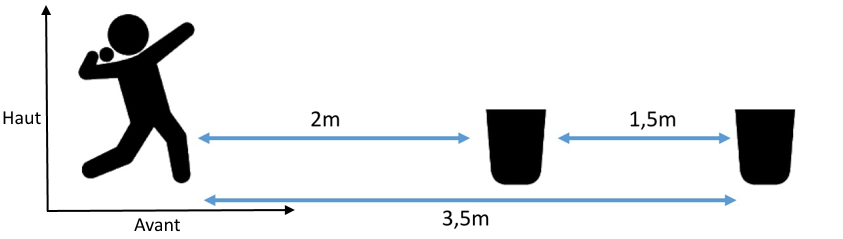
\includegraphics[width=\textwidth]{pictures/ball_throwing.png}
    \caption{Schéma de l'expérimentation du lancer de balle.}
    \label{fig:throwing_diagram}
\end{figure}

\subsection{Protocole}
Des instructions orales sont données quant à la tâche à effectuer : « Votre objectif est de lancer la balle dans une des deux corbeilles. Les cinquante premiers lancers devront viser la corbeille la plus proche, les cinquante autres la corbeille la plus éloignée. Vous êtes libre de lancer comme vous le souhaitez ». La personne retire ensuite tous les objets métalliques présents sur elle (ceinture, bracelets, téléphones, boucles d'oreilles, montres, etc.) afin d'éviter toute perturbation des capteurs (composés d'accéléromètres, de gyroscopes et de magnétomètres).

Le participant est ensuite mesuré selon les préconisations de NOITOM, afin de créer un squelette adapté selon douze mesures de distance suivantes :
\begin{itemize}
	\item Sommet du crâne jusqu'à la base du lobe de l'oreille / lèvre supérieure
	\item Base du lobe de l'oreille / lèvre supérieure jusqu'à la vertèbre C7
	\item Vertèbre C7 jusqu'au haut du fémur
	\item Largeur des épaules (épaule complète)
	\item Épaules (centre de rotation) jusqu'au coude (centre de rotation)
	\item Coude (centre de rotation) jusqu'au poignet (centre de rotation)
	\item Poignet (centre de rotation) jusqu'au bout du majeur
	\item Largeur des hanches (du fémur gauche jusqu'au fémur droit)
	\item Fémur jusqu'au genou (centre de rotation)
	\item Genou (centre de rotation) jusqu'à la cheville
	\item Cheville jusqu'au sol
	\item Talon jusqu'au bout du gros orteil
\end{itemize}

Une fois le squelette créé, les capteurs sont posés sur la personne. Le sujet se familiarise ensuite avec l'équipement, notamment en se déplaçant, afin de vérifier que la combinaison n'entrave pas ses mouvements. Cinq lancers sont ensuite réalisés avant le début de l'expérimentation, afin de se préparer et de s'habituer à l'équipement.

La combinaison est utilisée dans son intégralité, à l'exception des capteurs spécifiques aux doigts. En effet, nous avons constaté que l'utilisation de ces capteurs génère beaucoup de bruit dans les données de mouvement capturées, et ils ne sont pas nécessaires pour l'analyse réalisée.

Les calibrations sont ensuite effectuées afin d'étalonner les capteurs (position dans l'espace, espacement des capteurs entre eux, mise à zéro sur le logiciel de capture, etc.) pour que le logiciel puisse adapter la combinaison par rapport aux articulations du squelette 3D.

À chaque personne, il a été demandé de réaliser 100 lancers au total. Les 50 premiers lancers devaient viser la première corbeille, et les 50 autres devaient viser la seconde.

Une fois les lancers réalisés, l'export de chaque lancer au format BVH a été effectué. L'intervention humaine se borne à désigner le dossier contenant tous les fichiers de mouvements bruts. En premier lieu, les filtres sont appliqués. L'extraction des descripteurs fait suite à cette étape. La durée du chargement des fichiers BVH, le filtrage des descripteurs, l'extraction des descripteurs utilisés dans l'expérimentation et leur sauvegarde était d'environ 2 secondes par fichier sur une machine équipée d'un processeur 8 coeurs Intel Core i7-4910MQ 2.90GHz, 32Go de mémoire RAM tournant sous Windows 7.

Afin de vérifier la qualité du clustering, plusieurs métriques ont été utilisées en suivant principalement deux objectifs :
\begin{itemize}[label=$-$]
	\item évaluation interne des clusters, en assignant un score de vraisemblance pour chaque cluster, vérifiant la forme des clusters, leur cohésion, leur variance, etc.
	\item  évaluation externe des clusters, comparés les uns par rapport aux autres grâce à la distance les séparant, à l'aide d'une vérité terrain ou même d'une analyse experte \parencite{Jain1988ACD, Maulik2002Peo}
\end{itemize}

Afin de vérifier la séparabilité des données, la métrique utilisée est celle de l'Average Silhouette Score (\textit{ASS}) \parencite{Rousseeuw1987Sag}. Cette métrique se base sur le Silhouette Score (\textit{SS}) de chaque point individuel de donnée.

Soit $a(i)$ la distance moyenne d'un point $i$ par rapport à tous les autres points contenus dans le même cluster, définie par
\[a(i)={\frac {1}{|C_{i}|-1}}\sum _{j\in C_{i},i\neq j}d(i,j)\]
avec $d(i,j)$ la distance entre les points $i$ et $j$ au sein du cluster $C_i$. Cette mesure peut être considérée comme une indication de bonne appartenance du point $i$ au cluster $C_i$ : plus cette valeur est basse, plus le point $i$ est proche des autres points du cluster auquel il est assigné.

Soit $b(i)$ la distance moyenne minimale du point $i$ par rapport aux points des autres clusters (les distances moyennes étant calculées séparément pour chaque cluster ne contenant pas $i$), définie par
\[b(i)=\min _{k\neq i}{\frac {1}{|C_{k}|}}\sum _{j\in C_{k}}d(i,j)\]
avec $k$ étant le nombre de clusters.

Le Silhouette Score d'un point est défini par
\[s(i)={\frac {b(i)-a(i)}{\max\{a(i),b(i)\}}}, if |C_{i}|>1 |C_{i}|>1\]
et
\[s(i)=0, \text{si} |C_{i}|=1\]

L'Average Silhouette Score est la moyenne des Silhouette Scores de chaque échantillon du problème considéré. Ce score permet de mesurer dans quelle mesure l'échantillon appartient effectivement au cluster qui lui a été assigné, par rapport aux autres clusters. Cette valeur permet d'obtenir une estimation de l'homogénéité des clusters : une valeur élevée indique que les clusters sont bien séparés, alors qu'une valeur faible indique que les clusters sont proches, voire se superposent. Cette valeur varie entre -1 et 1 : une valeur de 1 signifie que tous les échantillons d'un cluster sont proches les uns des autres (les clusters sont bien séparés), alors qu'une valeur de 0 signifie que les clusters sont superposés. Dans ce dernier cas, une explication possible réside dans le nombre trop élevé ou trop faible de clusters. Struyf \textit{et al.} \parencite{Struyf1997Cia} ont proposé quatre paliers pour les valeurs de l'\textit{ASS} :
\begin{itemize}
	\item entre 0 et 0.25, aucune structure n'est discernable au sein des données
	\item entre 0.25 et 0.50, il existe une structure, bien que mal définie, voire artificielle
	\item entre 0.50 et 0.70, une structure existe au sein des données (séparation correcte des clusters)
	\item au-delà de 0.70, une structure est clairement définie au sein des données (très bonne séparation des clusters)
\end{itemize}

Dans le contexte de l'expérimentation, cette métrique permet donc de vérifier si les données sont séparables selon les descripteurs choisis.

S'il y a une séparation acceptable, il est nécessaire de déterminer les propriétés menant à cette séparation. Une approche consiste à corréler cette séparation avec le degré de réussite du geste. Dans le cas présent, ce degré est binaire : soit le geste est réussi (la balle a atterri dans la corbeille désignée), soit le geste est raté (la balle n'a pas atterri dans la corbeille désignée). En outre, il est aussi possible de considérer le type de lancer effectué ou la corbeille visée. Dans tous les cas, il faut disposer \textit{a priori} d'une vérité terrain, afin de pouvoir comparer le résultat du clustering à cet étiquetage. Dans ce contexte, plusieurs métriques ont été retenues : le rappel, la précision, le F1-score et l'Adjusted Rand Index (\textit{ARI}). Dans un problème de classification, le rappel indique la proportion d'éléments corrects contenus au sein de tous les éléments retournés, alors que la précision indique la proportion d'éléments corrects retournés par rapport au nombre d'éléments corrects total. Le F1-score correspond à la moyenne harmonique de ces deux valeurs. La valeur du F1 score se situe entre 0 et 1, avec une valeur de 1 indiquant une correspondance parfaite entre la séparation obtenue et la vérité terrain. Cependant, ce score n'est qu'une moyenne du F-score de chaque caractéristique de l'échantillon considéré. Ainsi, la valeur obtenue ne correspond pas au pouvoir discriminant des caractéristiques prises ensemble (information mutuelle) \parencite{Chen2006CSw}. %De plus, ce score donne une importance égale au rappel et à la précision ; en pratique, ce coût n'est pas toujours considéré comme égal \parencite{Hand2018Ano}.

L'\textit{ARI} est une mesure de similarité entre deux partitionnements de données différents \parencite{Morey1984ARI}. Cette mesure se base sur le Rand Index (RI) \parencite{Rand2971RI}. Soit un ensemble de $n$ données $E = {e_1, e_2, \ldots, e_n}$ et deux partitionnements de $E$ à comparer, avec $A = {A_1, \ldots, A_i}$ un partitionnement de $E$ en $i$ partitions et $B = {B_1, \ldots, B_j}$ un partitionnement de $E$ en $j$ partitions. On définit
\begin{itemize}
	\item $a$ comme étant le nombre de paires d'éléments dans $E$ qui se trouvent dans la même partition dans $A$ et dans $B$
	\item $b$ comme étant le nombre de paires d'éléments dans $E$ qui se trouvent dans des partitions différentes dans $A$ et dans $B$
	\item $c$ comme étant le nombre de paires d'éléments dans $E$ qui se trouvent dans la même partition dans $A$ et dans des partitions différentes dans $B$
	\item $d$ comme étant le nombre de paires d'éléments dans $E$ qui se trouvent dans des partitions différentes dans $A$ et dans la même partition dans $B$
\end{itemize}

Le Rand Index est défini par

\[ RI = \frac{a+b}{a+b+c+d} \]

Le dénominateur correspond au nombre total de paires d'éléments présents dans $E$. L'Adjusted Rand Index est une version normalisée du Rand Index \parencite{Hubert1985Cp}. Si on considère les mêmes éléments qu'auparavant (un ensemble de données $E$, et deux partitionnements $A$ et $B$), on peut créer un tableau de contingence comme suit :

\[
\begin{array}{c|cccc|c}
A \setminus B&B_{1}&B_{2}&\ldots &B_{j}&{\text{Sommes}}\\\hline
A_{1}&n_{11}&n_{12}&\ldots &n_{1l}&a_{1}\\
A_{2}&n_{21}&n_{22}&\ldots &n_{2l}&a_{2}\\
\vdots &\vdots &\vdots &\ddots &\vdots &\vdots \\
A_{i}&n_{i1}&n_{i2}&\ldots &n_{ij}&a_{j}\\\hline
{\text{Sommes}}&b_{1}&b_{2}&\ldots &b_{j}&
\end{array}
\]

Chaque case $n_{ij}$ indique le nombre d'éléments communs entre $A_i$ et $B_j$. L'Adjusted Rand Index est défini par la formule
\[ARI={\frac {\sum _{ij}{\binom {n_{ij}}{2}}-[\sum _{i}{\binom {a_{i}}{2}}\sum _{j}{\binom {b_{j}}{2}}]/{\binom {n}{2}}}{{\frac {1}{2}}[\sum _{i}{\binom {a_{i}}{2}}+\sum _{j}{\binom {b_{j}}{2}}]-[\sum _{i}{\binom {a_{i}}{2}}\sum _{j}{\binom {b_{j}}{2}}]/{\binom {n}{2}}}}\]

La valeur maximale est 1, et indique une correspondance parfaite entre les deux partitionnements de données. Une valeur de 0 correspond à une affectation aléatoire des données, et il est possible d'obtenir des valeurs négatives dans certains cas, dû à la normalisation \parencite{Meila2007Cca}.

Dans le contexte de l'expérimentation, ces métriques permettent de vérifier que le clustering obtenu correspond ou non à une séparation selon un étiquetage binaire.

\subsection{Données capturées}
Pour chaque lancer, le squelette de l'apprenant est capturé. Les mains sont représentées à l'aide d'un seul capteur. La réussite ou non du geste (la balle atterrit dans la corbeille désignée) est notée, ainsi que la corbeille visée et le type de lancer effectué.

\subsection{Données et métriques utilisées}
Pour chaque personne, 100 mouvements ont été enregistrés. Ces données sont enregistrées dans un format brut propriétaire de NOITOM (format RAW), puis exportées au format BVH (format ouvert d'animation de personnages, voir Chapitre \ref{chap:traitement_donnees}, section \ref{subsec:bvh}). Plusieurs descripteurs ont été extraits des mouvements, ayant chacun une valeur pour le début, la fin et l'indice de la valeur maximale de la vitesse moyenne de la main dominante :
\begin{itemize}
	\item la norme du vecteur vitesse (SN),
	\item la norme du vecteur vitesse en X, Y, Z (S x/y/z),
	\item la direction du vecteur vitesse en X, Y, Z (Sd x/y/z),
	\item la norme du vecteur vitesse ainsi que la direction de ce vecteur en X, Y, Z (SNDxyz).
\end{itemize}

L'utilisation des descripteurs liés à la vitesse se base sur l'hypothèse que la vitesse à imprimer à la balle afin de correctement viser la corbeille désignée serait différent selon la corbeille choisie. De plus, viser la corbeille la plus éloignée nécessite une force plus élevée, comparativement à la corbeille la plus proche. Enfin, les principales différences entre les types de lancers observés se situent au niveau de la direction de la balle, sa trajectoire ainsi que la force appliquée.

Plusieurs articulations ont été utilisées (alignée avec la préférence manuelle de la personne, gaucher ou droitier), correspondant aux parties du corps sollicitées lors du mouvement :
\begin{itemize}
	\item la main,
	\item l'avant-bras,
	\item le bras,
	\item l'épaule.
\end{itemize}
L'utilisation de plusieurs articulations permet de vérifier s'il existe d'une part une ou des articulations plus importantes pour la lancer, et d'autre part si la combinaison de descripteurs vitesses issus de plusieurs articulations permet d'augmenter la précision du clustering.

\subsection{Résultats}
Les résultats obtenus sont ceux d'une seule personne (100 lancers). L'utilisation de données de mouvement provenant d'une seule personne permet de limiter la variabilité des gestes de lancers : une fois un geste permettant de correctement viser la corbeille trouvé, les lancers suivants essayeront de reproduire les propriétés de ce lancer. Ainsi, on peut s'attendre à des données rapprochées (au sens des caractéristiques extraites) pour les lancers concernant une même corbeille. Le tableau \ref{throwing_results} présente les métriques calculées sur les clustering obtenus. Dans le cas des métriques de comparaison à une vérité terrain, les résultats sont donnés pour un clustering avec nombre de clusters $k = 2$. Les résultats pour la métrique permettant de vérifier la séparation des clusters sont également donnés pour $k = 2$, car c'est la valeur de $k$ qui donne les meilleurs résultats (quand la valeur $k = 2$ ne donne pas le meilleur résultat pour l'\textit{ASS}, les variations de cette valeur sont de l'ordre du centième, quelle que soit la valeur de $k$).

\begin{landscape}
\begin{table}[]
\centering
\begin{tabular}{|l|l|l|l|l|l|l|l|l|l|l|l|l|l|l|l|}
\hline
Joints & \multicolumn{5}{c|}{H}            & \multicolumn{5}{c|}{H, FA}        & \multicolumn{5}{c|}{H, FA, A}     \\ \hline
Metric & ASS  & P    & R    & F1   & ARI   & ASS  & P    & R    & F1   & ARI   & ASS  & P    & R    & F1   & ARI   \\ \hline
       & \multicolumn{15}{c|}{All data (ground truth = success / fail)}                                              \\ \hline
SN     & \cellcolor{green!25} 0.59 & 0.51 & 0.89 & 0.64 & 0.01  & 0.60 & 0.50 & 0.86 & 0.63 & 0.00  & 0.60 & 0.50 & 0.86 & 0.63 & 0.00  \\ \hline
Sxyz   & \cellcolor{green!25} 0.56 & 0.48 & 0.89 & 0.62 & -0.01 & 0.54 & 0.48 & 0.89 & 0.62 & -0.01 & 0.54 & 0.48 & 0.89 & 0.62 & -0.01 \\ \hline
Sdxyz  & 0.23 & 0.41 & 0.25 & 0.31 & -0.01 & 0.23 & 0.54 & 0.77 & 0.64 & 0.04  & 0.24 & 0.55 & 0.77 & 0.64 & 0.05  \\ \hline
SNDxyz & 0.26 & 0.53 & 0.89 & 0.67 & 0.04  & 0.27 & 0.55 & 0.77 & 0.64 & 0.05  & 0.26 & 0.53 & 0.77 & 0.63 & 0.03  \\ \hline
       & \multicolumn{15}{c|}{All data (ground truth = closest / farthest bin)}                                     \\ \hline
SN     & \cellcolor{green!25} 0.59 & 0.65 & 1.00 & 0.79 & 0.21  & 0.60 & 0.64 & 0.98 & 0.78 & 0.19  & 0.60 & 0.64 & 0.98 & 0.78 & 0.19  \\ \hline
Sxyz   & \cellcolor{green!25} 0.56 & 0.54 & 0.88 & 0.67 & 0.01  & 0.54 & 0.54 & 0.88 & 0.67 & 0.01  & 0.54 & 0.54 & 0.88 & 0.67 & 0.01  \\ \hline
Sdxyz  & 0.23 & 0.65 & 0.34 & 0.45 & 0.02  & 0.23 & 0.68 & 0.86 & 0.76 & 0.20  & 0.24 & 0.69 & 0.86 & 0.77 & 0.22  \\ \hline
SNDxyz & 0.26 & 0.68 & 0.98 & 0.80 & 0.26  & 0.27 & 0.71 & 0.88 & 0.79 & 0.26  & 0.26 & 0.69 & 0.88 & 0.77 & 0.22  \\ \hline
       & \multicolumn{15}{c|}{All data (ground truth = throwing type)}                                              \\ \hline
SN     & \cellcolor{green!25} 0.59 & 0.87 & 0.95 & 0.91 & \textbf{0.83}  & 0.60 & 0.83 & 0.95 & 0.89 & 0.79  & 0.60 & 0.83 & 0.95 & 0.89 & 0.79  \\ \hline
Sxyz   & \cellcolor{green!25} 0.56 & 0.06 & 0.05 & 0.05 & -0.09 & 0.54 & 0.06 & 0.05 & 0.05 & -0.09 & 0.54 & 0.06 & 0.05 & 0.05 & -0.09 \\ \hline
Sdxyz  & 0.23 & 0.08 & 0.10 & 0.09 & -0.07 & 0.23 & 0.54 & 0.95 & 0.69 & 0.39  & 0.24 & 0.53 & 0.95 & 0.68 & 0.37  \\ \hline
SNDxyz & 0.26 & 0.74 & 0.95 & 0.83 & 0.68  & 0.27 & 0.55 & 1.00 & 0.71 & 0.42  & 0.26 & 0.56 & 0.95 & 0.70 & 0.42  \\ \hline
\end{tabular}
\caption{Métriques calculées sur les résultats du clustering pour le lancer de balle.}
\label{throwing_results}
\end{table}
\end{landscape}

L'ajout d'articulations n'améliore pas (ou de manière marginale) la séparation des clusters dans tous les cas (valeurs d'$ASS$ et d'$ARI$ stables ou diminuant lors d'ajout d'autres articulations). Cela montre que la main reste l'articulation la plus discriminante pour la séparation des gestes. Dans le cas de la réussite ou non du geste, bien qu'une séparation acceptable soit possible à l'aide de la norme du vecteur vitesse ($ASS \approx 0.60$ pour les meilleurs cas), ainsi que les vecteurs vitesses en x, y et z, cette séparation ne correspondait pas au degré de réussite du geste ($ARI \approx 0$).

Pour la corbeille ciblée, les mêmes tendances se dégagent pour la séparation des clusters. Cette fois, l'\textit{ARI} obtient des valeurs $\approx 0.25$, suggérant une légère correspondance des regroupements avec l'étiquetage. Cependant, les valeurs d'\textit{ASS} correspondantes sont aux alentours de $0.25$, suggérant une mauvaise séparation des clusters.

Il est intéressant de noter qu'il a été possible d'obtenir à la fois une valeur correcte pour l'\textit{ASS} (0.59) et une valeur élevée pour l'\textit{ARI} (0.83) pour la séparation par rapport au type de lancer, avec le descripteur de la norme du vecteur vitesse. Cette corrélation entre une bonne valeur pour l'\textit{ASS} et une forte valeur pour l'\textit{ARI} suggère qu'il est possible, à l'aide des descripteurs et des méthodes utilisées, de séparer les gestes selon un critère observable par un humain. Ainsi, l'hypothèse \textbf{H1} a été validée dans le contexte de cette expérimentation. Cependant, cette séparation n'est pas corrélée avec le degré de réussite du geste, et l'hypothèse \textbf{H2} n'a pas pu être validée au cours de cette expérimentation. Une autre expérimentation a été conduite, afin de se focaliser sur la séparation du geste en fonction du résultat obtenu.

\section{Bottle Flip Challenge}
Le Bottle Flip Challenge est un défi qui provient de la performance d'un étudiant lors d'un concours de talents américain, au sein du lycée Ardrey Kell \parencite{BottleFlipChallengeOrigin}. L'étudiant de 18 ans, Mike Senatore, a offert au public une performance inattendue : un lancer de bouteille, partiellement remplie, qui réalise un salto arrière, avant de retomber parfaitement droite, sur la table (Fig. \ref{fig:BFC_example}). Filmé à l'aide d'un smartphone, la vidéo se propage rapidement sur internet, et de nombreuses personnes s'y essayent : le \textit{Bottle Flip Challenge} était né.

Ce mouvement possède l'avantage de ne nécessiter que peu de matériel : une bouteille d'eau partiellement remplie et une table. La durée du mouvement est également très courte, ce qui permet d'enregistrer beaucoup de données en un temps réduit. De plus, le geste ne nécessite pas de connaissance \textit{a priori}, ce qui fait qu'il n'est pas nécessaire d'avoir à disposition des personnes ayant déjà réalisé ce geste.

\begin{figure}
	\centering
    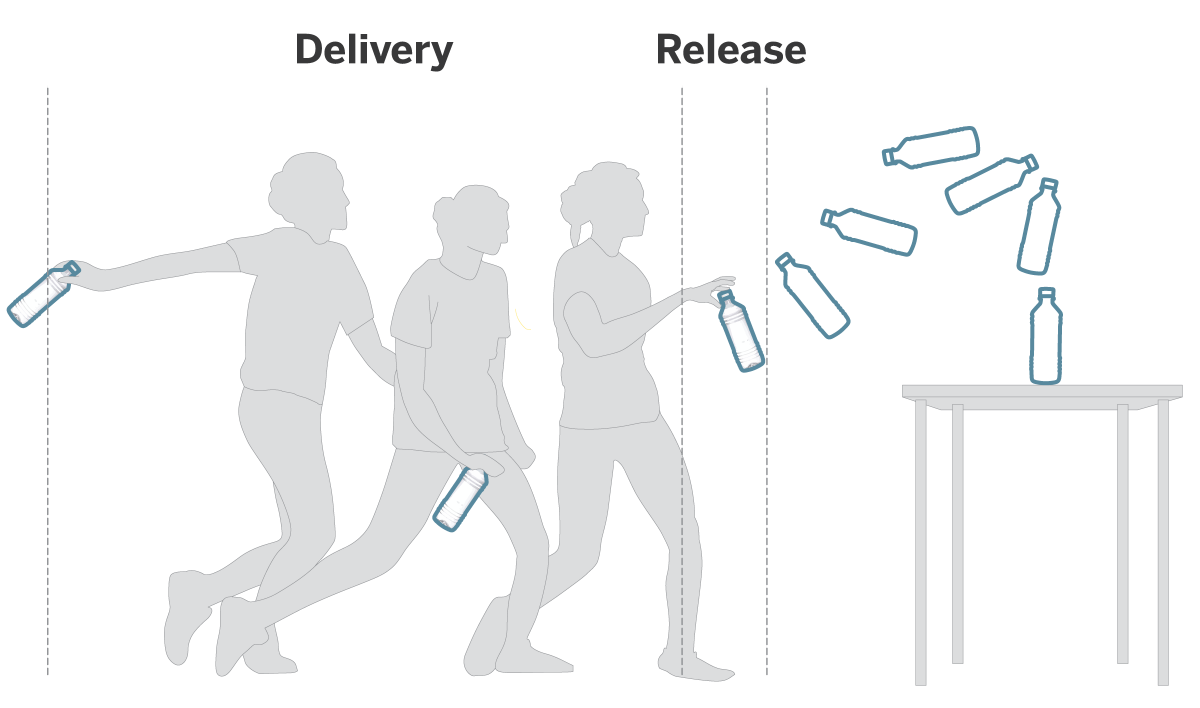
\includegraphics[width=\textwidth]{pictures/BFC_example.png}
    \caption[Exemple du mouvement du Bottle Flip Challenge]{Exemple du mouvement du Bottle Flip Challenge \protect\footnotemark.}
    \label{fig:BFC_example}
\end{figure}


Le mouvement de la bouteille, ainsi que de l'eau au sein de la bouteille, ont fait l'objet d'une étude récente \parencite{Dekker2018BF}. Il en ressort que les phénomènes physiques les régissant sont complexes et nombreux : dynamique des fluides, mouvement du projectile, moment cinétique, force centripète et gravité. Il ressort de cette étude scientifique que le lancer optimal présente un centre d'inertie bas, une vitesse angulaire faible et que le taux de remplissage optimal pour la bouteille se situe entre $20$ et $40$ \% de sa capacité maximale. Une autre étude \parencite{BFCAnalysis} montre qu'une bonne manière de lancer pour le Bottle Flip Challenge est de ne donner qu'une faible impulsion vers l'avant, et de lâcher la bouteille lorsqu'elle se trouve perpendiculaire au sol.

\subsection{Motivations et objectifs}
L'objectif de cette expérimentation était de déterminer s'il était possible d'obtenir une séparation des données en deux clusters, correspondant au degré de réussite du geste. Pour que le geste soit considéré comme réussi, il faut que la bouteille soit debout, sur la table, après avoir réalisé une rotation. L'hypothèse correspondante est la suivante :

\begin{itemize}
	\item \textbf{H2} : Il est possible de séparer les gestes des apprenants en deux groupes correspondant à une dichotomie geste réussi / geste raté afin de déterminer, pour une situation d'apprentissage donnée, les propriétés d'un ensemble fini de gestes réussis.
\end{itemize}

\footnotetext{https://wadsworthbruin.com/2016/12/01/bottle-flipping-into-the-heart-of-wadsworth-high/}

\subsection{Protocole}
La personne participante doit remplir un pré-questionnaire, contenant des informations sur le nom, l'âge, la taille, les connaissances par rapport au Bottle Flip Challenge. Des instructions orales sont données : \linebreak
\og Le but de cette expérience est de lancer une bouteille, de manière à ce qu’elle fasse un tour sur son axe horizontal avant de retomber correctement sur la table. Vous êtes libre sur la position de votre corps et le geste de lancer. Cependant, voici le geste communément utilisé pour réussir le lancer [faire une démonstration]. Il vous est demandé de vous mettre droit, les pieds avant la marque au sol, les bras le long du corps, la bouteille tenue dans votre main. Lorsque le premier bip retentira, vous lancerez la bouteille. Une fois le lancer terminé, vous remettrez les bras le long du corps, et attendrez que le deuxième bip retentisse avant de la reprendre, puis de vous remettre en position. Je vous signalerai lorsque vous aurez réalisé suffisamment de lancers. \fg

La personne retire ensuite tous les objets métalliques présents sur elle (ceinture, bracelets, téléphones, boucles d'oreilles, montres, etc.).

La personne est mesurée selon les préconisations de NOITOM \parencite{Noitom2015Doc}, pour qu'un squelette adapté soit créé. Une fois le squelette créé, les capteurs sont posés sur la personne. Le sujet se familiarise ensuite avec l'équipement, notamment en se déplaçant, afin de vérifier que la combinaison n'entrave pas le mouvement. Cinq lancers sont ensuite réalisés avant le début de l'expérimentation, pour se préparer, s'habituer à l'équipement et vérifier que le gant de la combinaison ne gêne pas la prise de la bouteille. L'installation complète est visible sur la figure \ref{fig:BFC_diagram}.

\begin{figure}
	\centering
    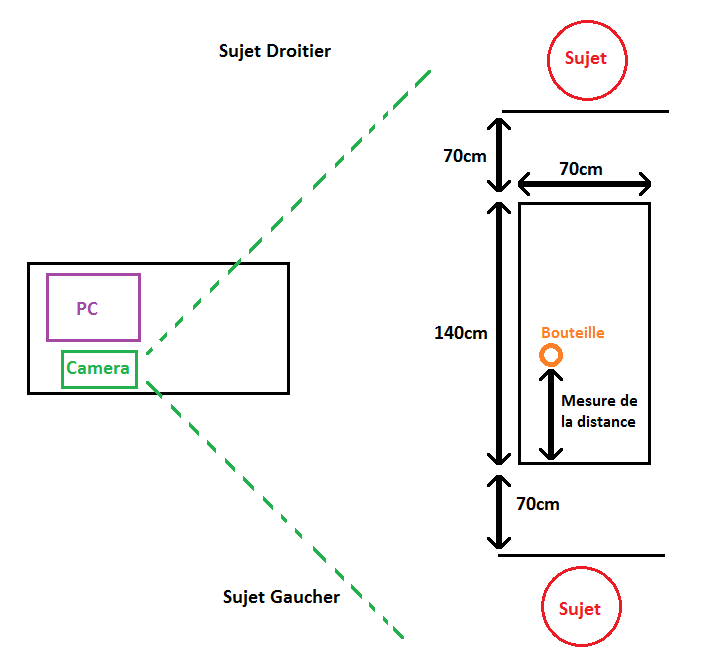
\includegraphics[width=\textwidth]{pictures/BFC_diagram.png}
    \caption{L'installation du matériel lors de l'expérimentation du Bottle Flip Challenge (vue du dessus).}
    \label{fig:BFC_diagram}
\end{figure}

Une fois les données de mouvement capturées, le même processus que pour la précédente expérimentation est utilisé afin d'importer, de filtrer, d'extraire les descripteurs et de sauvegarder les données ainsi extraites.

Les métriques utilisées pour analyser les résultats sont les mêmes que pour la précédente expérimentation.

\subsection{Données capturées}
Pour chaque lancer, le squelette de l'apprenant est capturé, y compris le mouvement des doigts. La réussite ou non du geste (bouteille qui atterrit correctement ou non après le salto arrière) est notée, et pour les gestes réussis, la distance de la bouteille par rapport au bord de la table où se situe la personne est mesurée.

\subsection{Données et métriques utilisées}
13 personnes au total ont participé à l'expérimentation. Pour chacune d'entre elles, 100 mouvements ont été enregistrés. Ces données sont enregistrées au format RAW de NOITOM, puis exportées dans le format BVH. Les mêmes descripteurs que précédemment ont été extraits, et les mêmes combinaisons d'articulations ont été utilisées.

L'hypothèse est que la vitesse de la bouteille est l'indicateur prédominant dans la réussite du geste : une vitesse trop faible ne permettrait pas à la bouteille de faire une rotation complète, et une vitesse trop élevée induirait plusieurs rotations, ainsi qu'un atterrissage non maîtrisé. La direction est utilisée afin de vérifier l'hypothèse que la direction du lancer influait également sur la réussite du geste.

\subsection{Résultats}
Dans le cas des métriques de comparaison à une vérité terrain, les résultats sont donnés pour un clustering avec nombre de clusters $k = 2$. Les résultats pour la métrique permettant de vérifier la séparation des clusters sont également donnés pour $k = 2$, car c'est la valeur de $k$ qui donne les meilleurs résultats (quand la valeur $k = 2$ ne donne pas le meilleur résultat pour l'\textit{ASS}, les variations de cette valeur sont de l'ordre du centième, quelle que soit la valeur de $k$). Lors de cette expérimentation, la combinaison de capteurs présentait beaucoup plus d'artefacts sur les articulations allant de l'épaule à la main sur le côté gauche. Les données des personnes gauchères présentaient donc plus de bruits que les données des personnes droitières. Ainsi, il a été décidé de faire les tests avec :

\begin{enumerate}[label=(\roman*)]
	\item les données mixtes (1300 données),
	\item les gauchers seuls (200 données),
	\item les droitiers seuls (1100 données).
\end{enumerate}

Les résultats sont présentés dans le tableau \ref{BfC_results}.

\begin{landscape}

\begin{table}[]
\centering
\begin{tabular}{|l|l|l|l|l|l|l|l|l|l|l|l|l|l|l|l|}
\hline
Joints & \multicolumn{5}{c|}{H}           & \multicolumn{5}{c|}{H,FA}        & \multicolumn{5}{c|}{H, FA, A}    \\ \hline
Metric & ASS  & P    & R    & F1   & ARI  & ASS  & P    & R    & F1   & ARI  & ASS  & P    & R    & F1   & ARI  \\ \hline
& \multicolumn{15}{|c|}{Left and Right-Handed}                                                                    \\ \hline
SN     & 0.48 & 0.25 & 0.33 & 0.29 & 0.04 & 0.44 & 0.25 & 0.33 & 0.29 & 0.04 & 0.43 & 0.25 & 0.33 & 0.29 & 0.04 \\ \hline
Sxyz   & \cellcolor{green!25} 0.54 & 0.18 & 0.67 & 0.30 & 0.05 & 0.52 & 0.27 & 0.32 & 0.29 & 0.05 & 0.51 & 0.18 & 0.68 & 0.29 & 0.05 \\ \hline
Sdxyz  & 0.24 & 0.21 & 0.53 & 0.30 & 0.00 & 0.27 & 0.25 & 0.25 & 0.25 & 0.04 & 0.22 & 0.18 & 0.72 & 0.27 & 0.04 \\ \hline
SNDxyz & 0.21 & 0.18 & 0.47 & 0.30 & 0.00 & 0.27 & 0.25 & 0.26 & 0.26 & 0.04 & 0.22 & 0.26 & 0.28 & 0.27 & 0.04 \\ \hline
& \multicolumn{15}{|c|}{Left Handed}                                                                              \\ \hline
SN     & 0.41 & 0.39 & 0.39 & 0.39 & 0.02 & 0.42 & 0.38 & 0.39 & 0.39 & 0.01 & 0.41 & 0.31 & 0.61 & 0.39 & 0.01 \\ \hline
Sxyz   & 0.35 & 0.32 & 0.57 & 0.39 & 0.00 & 0.34 & 0.32 & 0.57 & 0.39 & 0.00 & 0.33 & 0.35 & 0.43 & 0.39 & 0.00 \\ \hline
Sdxyz  & 0.31 & 0.34 & 0.48 & 0.40 & 0.00 & 0.27 & 0.34 & 0.54 & 0.39 & 0.00 & 0.23 & 0.34 & 0.48 & 0.40 & 0.00 \\ \hline
SNDxyz & 0.27 & 0.34 & 0.49 & 0.40 & 0.00 & 0.25 & 0.33 & 0.48 & 0.39 & 0.00 & 0.22 & 0.34 & 0.52 & 0.41 & 0.00 \\ \hline
& \multicolumn{15}{|c|}{Right Handed}                                                                             \\ \hline
SN     & 0.42 & 0.18 & 0.29 & 0.22 & 0.00 & 0.36 & 0.17 & 0.28 & 0.21 & 0.00 & 0.34 & 0.17 & 0.28 & 0.21 & 0.00 \\ \hline
Sxyz   & \cellcolor{green!25} 0.73 & 0.19 & 0.12 & 0.15 & 0.01 & 0.71 & 0.19 & 0.12 & 0.15 & 0.01 & 0.71 & 0.19 & 0.12 & 0.15 & 0.01 \\ \hline
Sdxyz  & 0.28 & 0.15 & 0.45 & 0.28 & 0.00 & 0.20 & 0.16 & 0.49 & 0.27 & 0.00 & 0.26 & 0.19 & 0.13 & 0.15 & 0.01 \\ \hline
SNDxyz & 0.26 & 0.16 & 0.45 & 0.28 & 0.00 & 0.19 & 0.19 & 0.52 & 0.27 & 0.00 & 0.26 & 0.17 & 0.87 & 0.15 & 0.01 \\ \hline
\end{tabular}
\caption{Métriques calculées sur les résultats du clustering pour le Bottle Flip Challenge.}
\label{BfC_results}
\end{table}
\end{landscape}

Dans tous les cas, l'ajout d'autres articulations que celle de la main ne fait que rajouter du bruit (les valeurs de l'$ASS$ et l'$ARI$ décroissent). Les plus fortes valeurs d'\textit{ASS} (séparation des clusters) ont été obtenues pour les descripteurs vecteur vitesse en X, Y, Z ($ASS$ des descripteurs Sxyz $= 0.73$). On peut également remarquer que les résultats de l'\textit{ASS} sont meilleurs sur les données des droitiers seuls pour ces descripteurs, par opposition aux données mixtes ou des gauchers seulement (dernière partie du tableau \ref{BfC_results}). Cette tendance tend à confirmer les problèmes de capteurs du côté gauche de la combinaison. Le tableau 7 montre que les valeurs les plus discriminantes pour la séparation sont le vecteur vitesse en Z (en avant) et en Y (en haut) au moment de la vitesse maximale. Cette séparation est cohérente avec les études réalisées par \parencite{Dekker2018BF} et \parencite{BFCAnalysis} qui suggèrent que les différences entre un lancer réussi et raté se situent au niveau de la force et de la direction du lancer.

\begin{table}[]
\centering
\begin{tabular}{|l|l|l|l|}
\hline
            & Beginning & Maximum & End    \\ \hline
X (Side)    & 0.0398    & 0.5071  & 0.0110 \\ \hline
Y (Upward)  & 0.0415    & \cellcolor{green!25} 1.7497  & 0.0998 \\ \hline
Z (Forward) & 0.0847    & \cellcolor{green!25} 2.0477  & 0.0536 \\ \hline
\end{tabular}
\label{BfC_best_descriptors}
\caption[Distance relative entre les centroïdes des clusters, pour la main droite, avec les vecteurs vitesse en X, Y, Z pour $k = 2$.]{Distance relative entre les centroïdes des clusters, pour la main droite, avec les vecteurs vitesse en X, Y, Z pris au début, au maximum et à la fin du lancer, pour $k = 2$.}
\end{table}

Dans tous les cas, les valeurs de l'\textit{ARI} (correspondance avec la vérité terrain) sont restées proches de 0, ce qui indique que les séparations obtenues ne correspondaient pas au degré de réussite du geste. Ainsi, l'hypothèse \textbf{H2} n'a pas été validée au cours de cette expérimentation.

Les descripteurs utilisés conjointement avec les algorithmes de clustering ne peuvent donc pas proposer un regroupement corrélé avec le degré de réussite du geste, dans le cas du \textit{Bottle Flip Challenge}. Le peu de variabilité du geste d'un lancer à un autre (et, par extension, d'un lancer réussi à un lancer raté) est une piste pour expliquer que l'algorithme des \textit{k-means} appliqué non récursivement n'est pas suffisant pour obtenir une telle séparation. De plus, les descripteurs utilisés dans cette expérimentation sont tous basés sur la vitesse. Ce type d'indicateurs semble ne pas être suffisant pour caractériser la réussite ou non du geste. Plusieurs autres descripteurs auraient pu être utilisés, tels que la courbure (indication sur la vitesse de changement d'une courbe au cours du temps), la vitesse angulaire des articulations sollicitées (poignet et main), ainsi que le déplacement du centre de masse de la personne, \textit{etc.} La complexité des phénomènes physiques régissant le lancer (autant pour le mouvement du bras et de la main que celui de l'eau dans la bouteille) peuvent également indiquer que les descripteurs basés vitesses ne sont pas suffisant pour caractériser tous les aspects du geste important pour un lancer réussi.

Plusieurs problèmes ont également émané de l'expérimentation elle-même. Premièrement, la distance entre la table et la personne lançant n'était pas systématiquement constante. En effet, certaines personnes prenaient un léger élan, ou se reculaient légèrement avant de lancer par rapport à la position limite imposée (voir figure \ref{fig:BFC_diagram}). De plus, il n'était pas possible de mesurer le point d'impact exact de la bouteille sur la table, car cette dernière glissait lors d'un lancer réussi. Cette distance n'a ainsi pas été considérée pour notre analyse. Bien que corrigée à l'aide de pré-traitements, l'imprécision des données de capture récoltées (cf. chapitre \ref{chap:traitement_donnees} section \ref{sec:traitements}) est également un facteur à prendre en compte dans les résultats obtenus.

\subsection{Discussion}
Ces deux premières expérimentations ont permis de vérifier la capacité de la plateforme MLA à traiter de manière automatique les données, une fois paramétrée selon les besoins d'analyse. Ces expérimentations ont également permis de vérifier s'il était possible d'obtenir automatiquement une séparation entre les gestes jugés réussis et ceux jugés ratés, pour un cas précis. Les descripteurs choisis, ainsi que la méthode utilisée, ont permis d'aboutir à une séparation des données acceptable dans les deux expérimentations.

Cependant, pour le \textit{Bottle Flip Challenge}, la séparation obtenue ne correspond pas à une dichotomie geste réussi/raté. Le manque d'analyse experte est un problème qui est apparu au cours de l'expérimentation. Bien que le Bottle Flip Challenge ait fait l'objet d'articles scientifiques sur la physique régissant le lancer et la bouteille \parencite{Dekker2018BF, BFCAnalysis}, il ne semble pas y avoir d'expertise formalisée du geste au moment où ces lignes sont écrites. En ce qui concerne l'étude du geste, la rotation du poignet aurait pu être une piste intéressante à explorer. Un sous-ensemble réduit de descripteurs a été utilisé pour cette expérimentation, ce qui a limité les résultats obtenus. Le calcul d'autres descripteurs (tels que ceux présentés dans \parencite{larboulette2015Descriptors} par exemple) aurait pu mener à de meilleurs résultats.

L'analyse du geste, dans le cas de ces deux expérimentations, se fait de manière binaire : soit le geste est acceptable, soit il ne l'est pas. Dans une situation d'apprentissage, il n'est pas toujours possible de regrouper ces mouvements dans ces deux catégories. Le degré de succès peut avoir une granularité plus fine, ou dépendre de l'acceptabilité binaire (ou non) de plusieurs autres propriétés du geste.

De plus, dans un tel processus, l'humain est écarté du processus d'analyse. Son expertise n'est utilisée qu'\textit{a priori}, et son intervention n'est pas requise dans le processus d'évaluation et \textit{in fine} de conseil pour l'apprentissage. Bien qu'un tel système puisse présenter des avantages, l'objectif est de proposer une aide à la décision pour l'enseignant/l'expert, et non pas un remplacement de ce dernier. Le système de retours de MLA, basé sur une analyse et une évaluation par regroupement des besoins d'observation du geste, permet de fournir un retour graphique à l'expert ou à l'apprenant. Ce système est l'objet de l'expérimentation suivante.

\section{Expérimentation : lancer de fléchettes}
Cette section présente l'évaluation de la partie de retours à l'apprenant du système MLA au travers d'une expérimentation portant sur le lancer de fléchettes. Il s'agit d'un sport où la technicité du geste est formalisée \footnote{\url{https://www.dartslive.com/enjoy/en/throw/}}. Il existe, pour chaque partie du corps impliquée, des explications précises quant à la position et au mouvement. Après une analyse de ces explications, nous proposons une représentation du geste sous la forme d'un ensemble de descripteurs représentant chaque besoin d'observation. Les valeurs d'acceptabilité de ces descripteurs sont ensuite estimées à l'aide d'un clustering basé sur les démonstrations de l'expert. Enfin, ces valeurs sont comparées à celles de l'apprenant afin de lui fournir un retour.

\subsection{Motivations et objectifs}
Les objectifs de cette expérimentation sont multiples. Il s'agit d'une part de montrer qu'il est possible, à l'aide du système de retours à l'apprenant basé sur les démonstrations de l'expert et l'estimation de valeurs d'acceptabilité empiriques des propriétés du geste, de donner des conseils pertinents lors de la réalisation de ces derniers. D'autre part, il s'agit également de montrer qu'une amélioration du geste, en termes de précision du tir et de la « forme » du mouvement résultait de ces conseils. Enfin, l'efficacité du système selon les modalités précédemment citées est évaluée en termes d'usage : utilisation du système seul, ou utilisation conjointe avec l'analyse de l'expert.

Les hypothèses correspondantes sont les suivantes :
\begin{itemize}
    \item \textbf{H3} : Il est possible de séparer les gestes en fonction de propriétés attendues et identifiées au préalable par l'expert.
	\item \textbf{H4} : Il est possible de corriger chaque défaut du geste de l'apprenant, en lui indiquant les défauts majeurs à corriger en premier. Un défaut majeur est identifié par la plus grande distance séparant le mouvement courant de l'apprenant, du groupe de gestes acceptables ayant éliminé ce défaut.
	\item \textbf{H5} : L'utilisation du système MLA basée sur l'hypothèse 4 permet d'améliorer l'apprentissage du geste par rapport à une situation sans le système MLA.
	\item \textbf{H6} : L'utilisation du système MLA en tant qu'assistant à l'enseignant permet d'améliorer l'apprentissage du geste par rapport à une situation sans MLA, et à une situation avec MLA et sans enseignant.
\end{itemize}


En conséquence, l'objectif pour les personnes réalisant l'expérimentation est de viser le centre de la cible, et également de suivre les conseils donnés par l'expert utilisant le système ou non.

Afin d'évaluer les résultats obtenus, trois groupes ont été formés : un groupe " contrôle ", où seul l'expert donne des conseils (système absent), un groupe où seul le système donne les conseils (évaluation experte absente), et un groupe où l'expert peut s'appuyer sur le système afin de décider des conseils à donner.

\subsection{Fléchettes : principes et description}
\subsubsection{Matériel}
Le lancer de fléchettes est un sport qui se pratique à l'aide d'une cible (Figures \ref{fig:darts_target} et \ref{fig:darts_zone}) et de fléchettes (Fig. \ref{fig:single_dart}). La cible est constituée de vingt zones distinctes et de tailles égales, numérotées de 1 à 20, ainsi que d'un cercle au centre (Fig. \ref{fig:darts_target}). Chacune des zones est également divisée (Fig. \ref{fig:darts_zone}) :

\begin{itemize}
	\item les simples sont les deux plus grandes parties d'une zone,
	\item les doubles se situent sur la couronne extérieure des zones,
	\item les triples se situent sur la couronne intérieure des zones.
\end{itemize}

Le double centre compte comme un " double " du centre simple ($2 \times 25$).

\begin{figure}
    \centering
    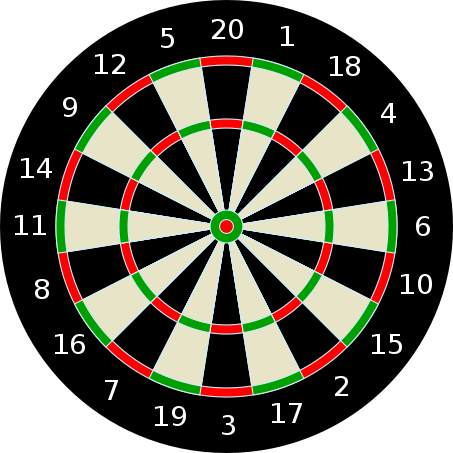
\includegraphics[width=5cm]{pictures/darts_target.png}
    \caption[Cible de fléchettes]{Une cible de fléchettes classique$^1$.}
    \label{fig:darts_target}
\end{figure}

\begin{figure}
    \centering
    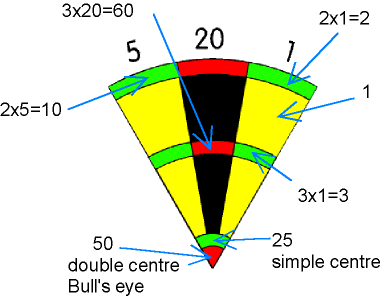
\includegraphics[width=5cm]{pictures/darts_zone.png}
    \caption[Zones d'une cible de fléchettes]{Détail des zones d'une cible de fléchettes classique$^1$.}
    \label{fig:darts_zone}
\end{figure}

\begin{figure}
    \centering
    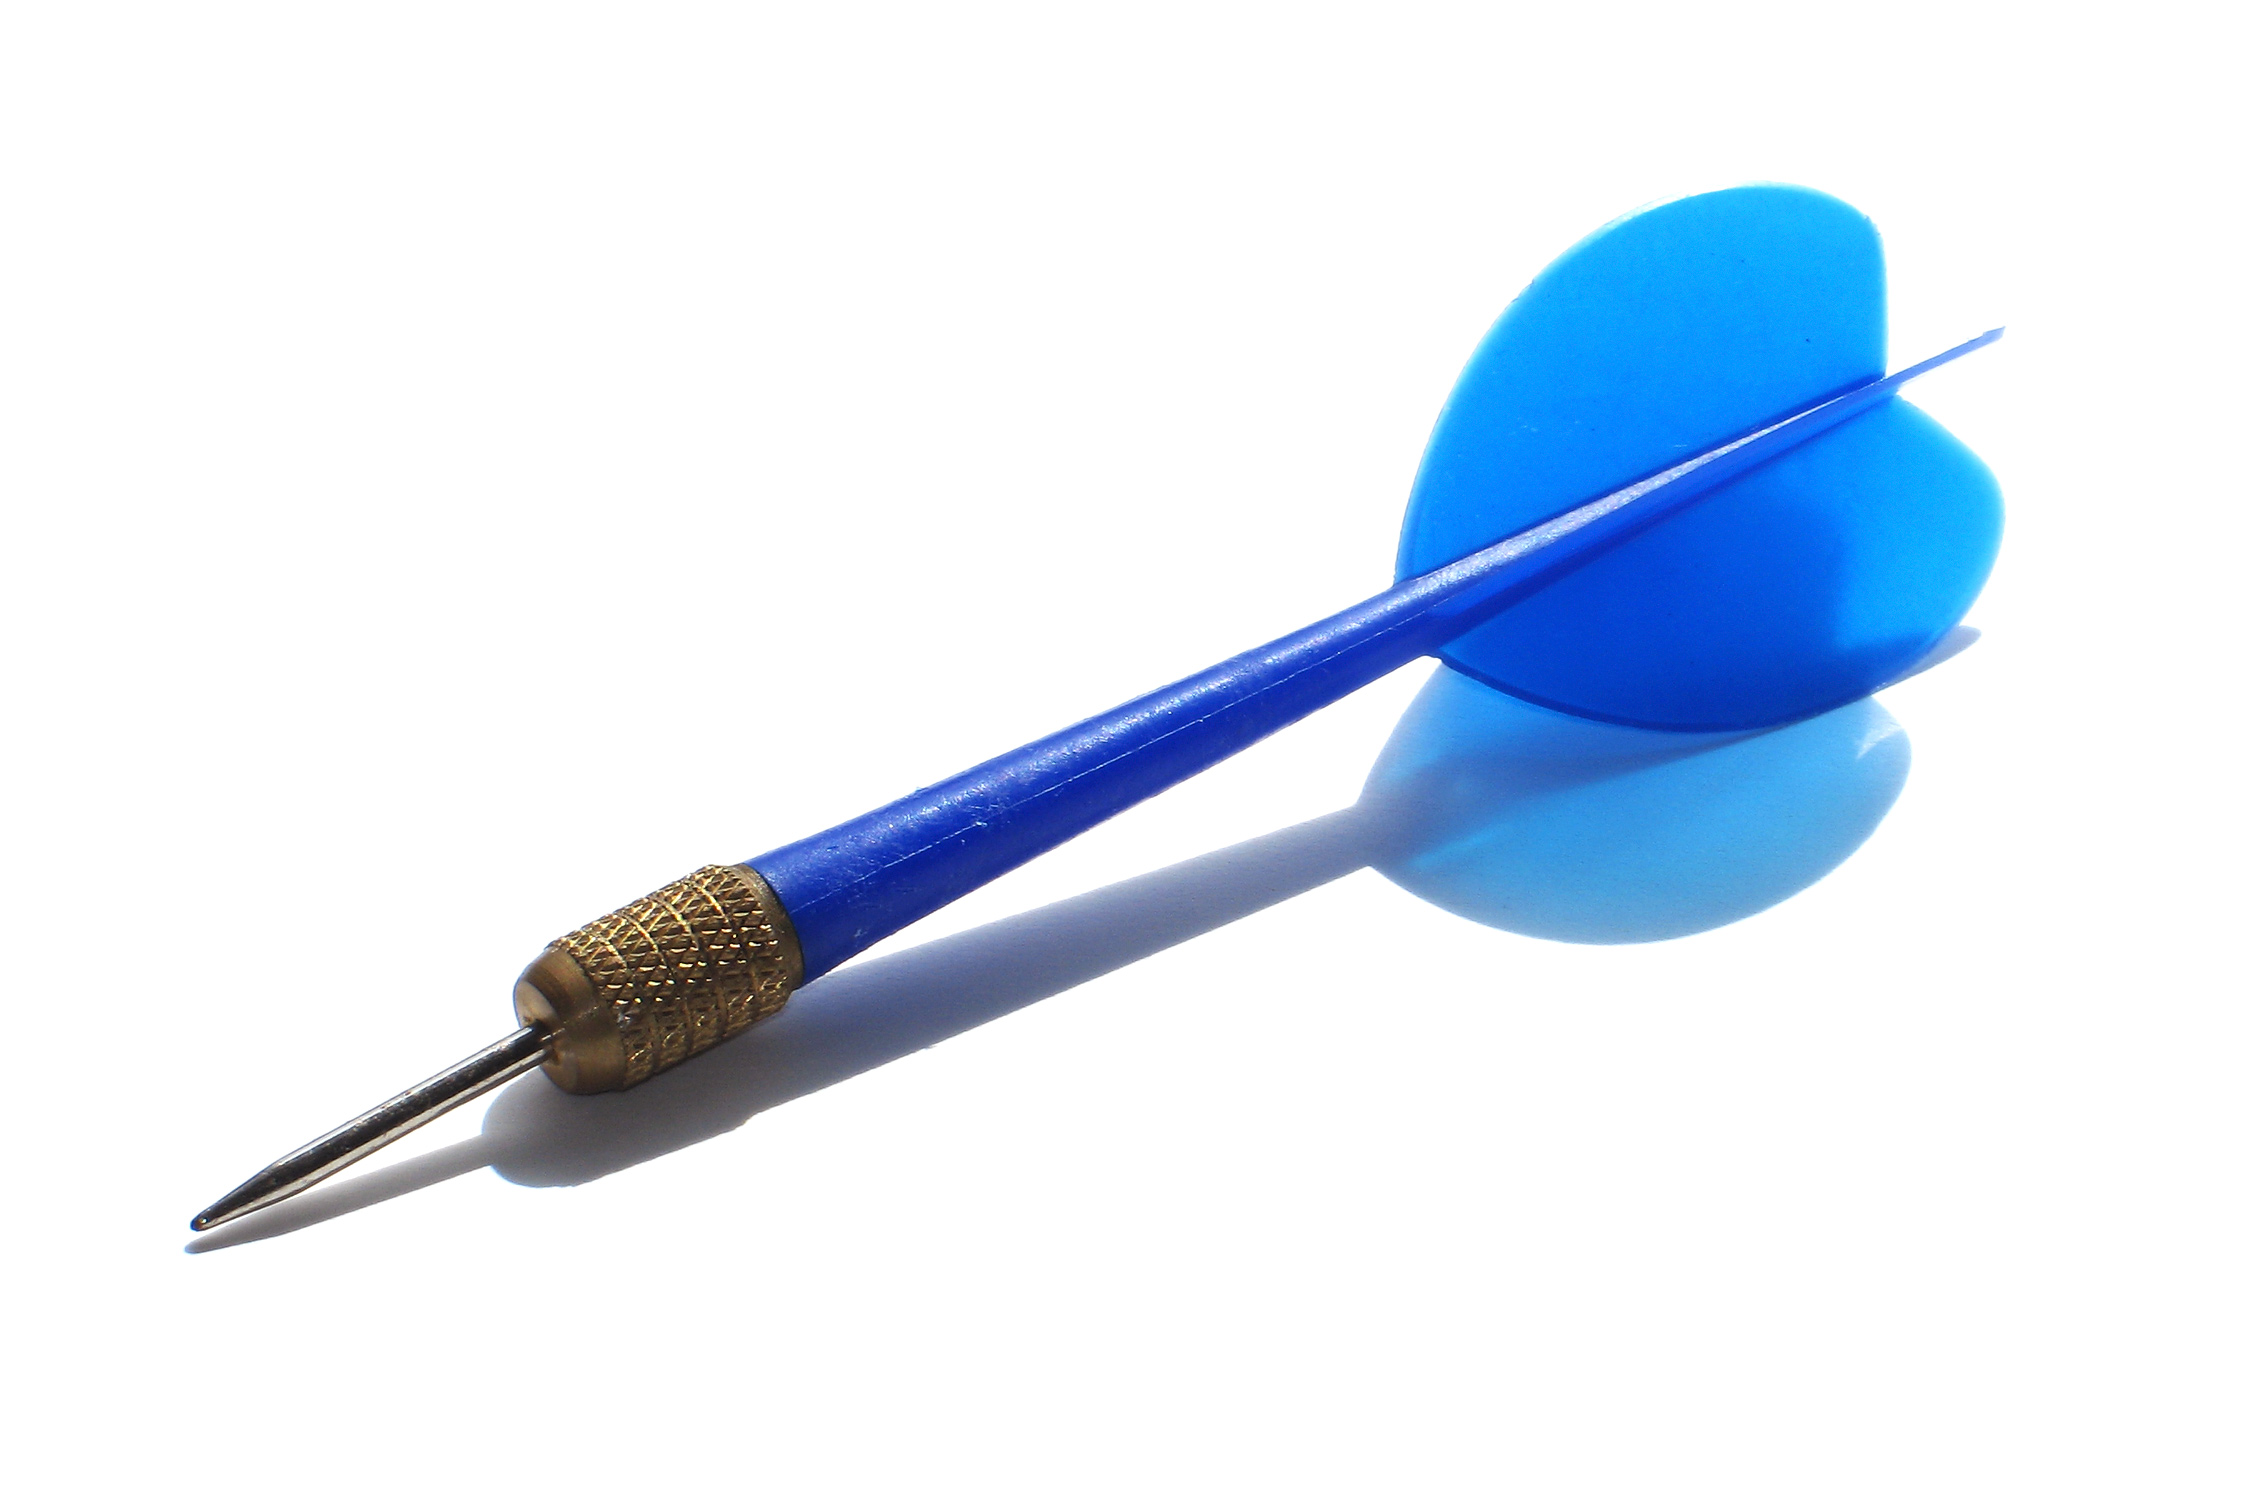
\includegraphics[width=5cm]{pictures/dart.jpg}
    \caption[Fléchette]{Exemple de fléchette respectant les normes officielles$^1$.}
    \label{fig:single_dart}
\end{figure}



La \textit{World Darts Federation} définit des critères à respecter pour l'installation et les parties de fléchettes. Ainsi, la cible doit respecter les dimensions suivantes :
\begin{itemize}
\item largeur intérieure des doubles et des triples : 8 mm
\item diamètre du centre (bulle) : 12,7 mm
\item diamètre du demi-centre (demi-bulle) : 31,8 mm
\item rayon du cercle extérieur de la couronne des doubles : 170 mm
\item rayon du cercle extérieur de la couronne des triples : 107,4 mm
\item diamètre total de la cible : 451 mm
\item épaisseur des fils : minimum 1,6 mm - maximum 1,8 mm
\end{itemize}

Le centre de la cible doit se trouver à 172,72 centimètres du sol, et la limite de tir est située à 2,37 mètres de la cible.

Les fléchettes doivent avoir une largeur inférieure à 3,38 centimètres et peuvent être de n'importe quelle longueur, tant que la distance allant de pointe au bout de l'empennage ne dépasse pas 20 centimètres. La masse d'une fléchette ne doit pas dépasser 50 grammes.

Les règles des différents jeux existants ne seront pas détaillées ici, car elles n'ont pas été utilisées dans le contexte de l'expérimentation. L'installation réalisée pour cette expérimentation respecte les dimensions et les distances imposées par la \textit{World Darts Federation}.

\footnotetext{source : https://fr.wikipedia.org/wiki/Fl\%C3\%A9chettes}

\subsubsection{Caractéristiques du mouvement et descripteurs considérés}
Des entretiens ont été réalisés avec un expert des fléchettes : Aurélien Orsini, président du \textit{Dart dart club de fléchettes mayennais} et champion régional en 2014. Ces entretiens ont pour but de prendre connaissance des modalités d'évaluation du geste de l'apprenant par l'expert lors d'une séance d'apprentissage, ainsi que des conseils prodigués pour améliorer le geste. Cette étape a permis de vérifier que les parties du corps et les modalités du mouvement regardées par l'expert sont formalisables en descripteurs opérationnalisables et en conséquence calculables à partir du mouvement enregistré. De ces entretiens sont ressortis quatre défauts majeurs souvent présents chez les débutants.

Le premier défaut est lié au fait de se pencher en avant (\textit{leaning}) durant le lancer. Lorsqu'un débutant lance une fléchette, son corps accompagne naturellement le geste en se penchant en avant (Fig. \ref{fig:darts_leaning_final})
. Ce défaut peut entraîner une visée plus basse que prévu, car le mouvement du corps imprime une rotation vers le bas au bras, par extension. Le conseil donné par l'expert est de rester fixe sur ses appuis, une fois en position de tir, tout en gardant le haut du corps (des hanches jusqu'à la tête) le plus immobile possible. Les descripteurs utilisés pour caractériser cet aspect du geste est la vitesse moyenne des épaules au cours du lancer : plus elle est basse, moins le haut du corps a bougé.

\begin{figure}
    \centering
    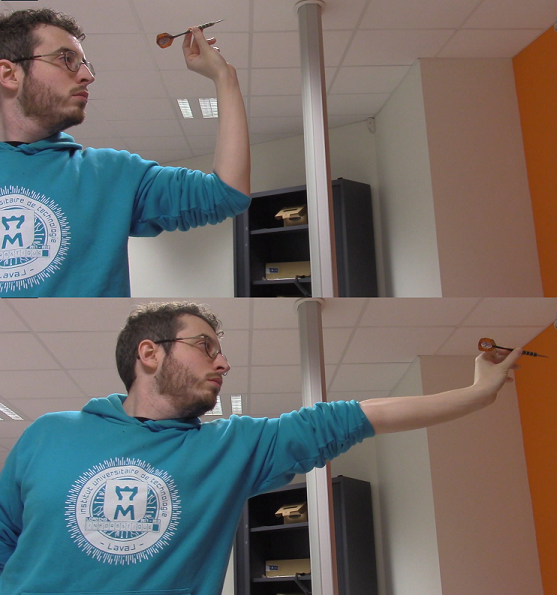
\includegraphics[width=10cm]{pictures/darts_leaning_final.png}
    \caption[Défaut du « leaning » (se pencher en avant)]{Défaut du « leaning » illustré : l'apprenant se penche en avant lors du lancer.}
    \label{fig:darts_leaning_final}
\end{figure}

Le deuxième défaut identifié est celui du mouvement du coude (\textit{elbow move}). Lors du lancer de fléchettes, le corps, ainsi que le bras, doivent rester le plus statique possible. Le mouvement de lancer doit s'effectuer à l'aide d'une rotation du coude, ce qui n'est possible que lorsque le bras est placé suffisamment en position de pré-lancer. Le problème usuel du geste d'un novice est que le bras et l'avant-bras forment un « V » avant le lancer, et finissent par former une ligne après le lancer, ce qui implique un déplacement du coude au cours du lancer. Le mouvement est ainsi moins maîtrisé que si le coude est la seule articulation qui pivote (Fig. \ref{fig:darts_elbow_move_final}). Le conseil donné par l'expert, dans ce cas, est de se concentrer sur l'immobilité du bras, afin que le coude effectue un pivot et que seul l'avant-bras ne bouge. Cet aspect du geste est caractérisé par les descripteurs de vitesse moyenne du coude, ainsi que de l'épaule (du côté de la préférence manuelle de l'utilisateur). Plus ces valeurs sont basses, moins le bras a bougé.

\begin{figure}
    \centering
    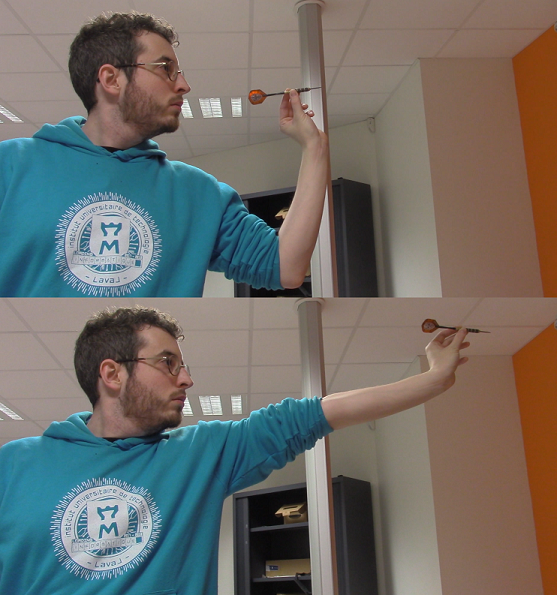
\includegraphics[width=10cm]{pictures/darts_elbow_move_final.png}
    \caption[Défaut du « elbow move » (déplacement du coude)]{Défaut du « elbow move » illustré : le coude de l'apprenant effectue un déplacement lors du lancer, au lieu de seulement effectuer une rotation.}
    \label{fig:darts_elbow_move_final}
\end{figure}

Un autre défaut possible est celui du " lancer de javelot " (\textit{javelin}). Lors d'un lancer, le bras, l'avant-bras et la main doivent rester devant le corps, dans l'alignement de l'axe tête-cible. Du début à la fin du mouvement, le bras, ainsi que la main, doivent toujours rester devant le corps. Or, chez les novices, le bras est souvent décalé (sur la gauche pour les gauchers, sur la droite pour les droitiers), et la prise d'élan du geste fait aller le bras à côté de la tête, voire même derrière (Fig. \ref{fig:darts_javelin_final}). Afin de détecter ce problème, la distance en x, y, et z de la main par rapport à la tête avant le lancer est utilisée.

\begin{figure}
    \centering
    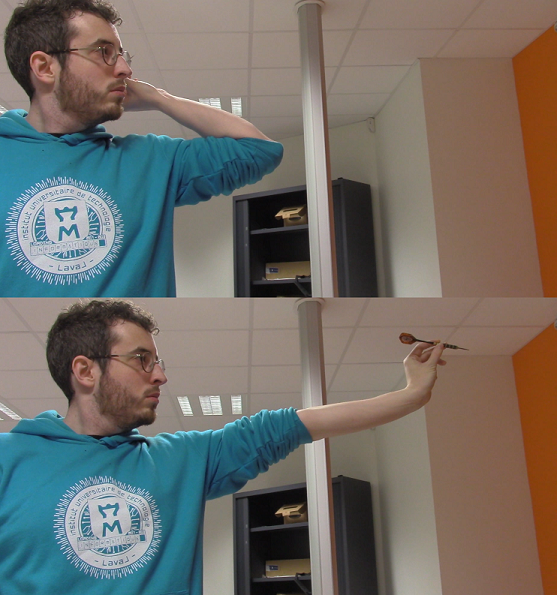
\includegraphics[width=10cm]{pictures/darts_javelin_final.png}
    \caption[Défaut du « javelin » (lancer en javelot)]{Défaut du « javelin » illustré : la main de l'apprenant passe à côté (voire derrière) la tête lors de la prise d'élan du lancer.}
    \label{fig:darts_javelin_final}
\end{figure}

Le dernier défaut est celui de l'alignement du bras (\textit{align arm}). Un phénomène naturel lors du lancer est d'avoir un décalage entre l'alignement initial du bras et l'alignement final (lors du lancer). En effet, le bras a naturellement tendance à revenir vers le centre du corps, quelle que soit la préférence manuelle de la personne (droitier ou gaucher) (Fig. \ref{fig:darts_align_arm_final}). Il faut consciemment compenser cet effet, en essayant de garder un alignement équivalent du début à la fin du lancer. Afin de vérifier cet aspect du geste, une boîte englobante est calculée sur l'ensemble du geste. La moyenne de la largeur de cette boîte, ainsi que l'écart type, sont ensuite utilisés.

\begin{figure}
    \centering
    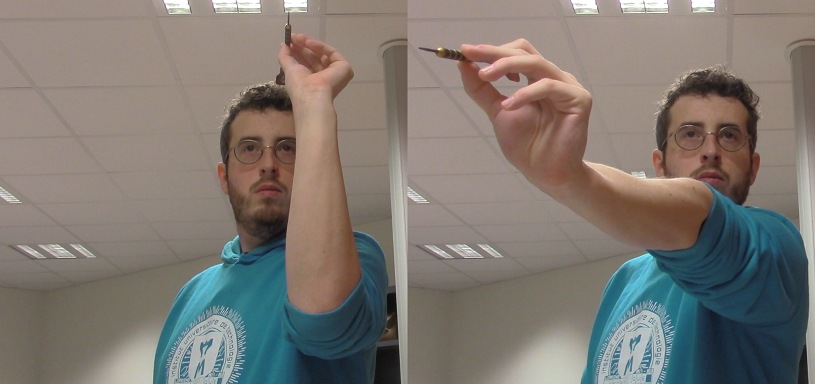
\includegraphics[width=10cm]{pictures/darts_align_arm_final.png}
    \caption[Défaut du « align arm » (alignement du bras)]{Défaut du « align arm » illustré : le bras de l'apprenant se dirige légèrement vers la droite lors du lancer (dans le cas d'un gaucher). L'effet inverse se produit pour un droitier.}
    \label{fig:darts_align_arm_final}
\end{figure}

Chaque défaut n'apparaît pas forcément indépendamment des autres : dans la réalité, les apprenants cumulent très souvent plusieurs de ces défauts. Il existe également d'autres défauts, tels que la mauvaise prise d'une fléchette, un mauvais relâchement de la fléchette (qui lui imprime un mouvement erratique), etc. Ces problèmes ne sont cependant pas détectables à l'aide du mouvement de l'apprenant seul. Ils nécessitent d'autres données (telles que la position de la fléchette, la connaissance du moment du lâcher de fléchette, etc.) qu'il n'est pas possible d'obtenir à l'aide du matériel utilisé pour cette expérimentation.

\subsection{Protocole}
\subsubsection{Acquisition des données de l'expert}
La première étape est la captation des données de l'expert, afin d'intégrer les besoins d'observation de l'expert au sein du système. L'objectif est d'obtenir des données correspondant à des mouvements jugés corrects par l'expert, et des données avec les défauts pris séparément. Ainsi, l'expert a réalisé dix lancers de fléchettes bons, puis dix lancers pour chacun des quatre défauts identifiés. Puis, pour chaque défaut, les descripteurs correspondants sur les bons mouvements, et sur les mouvements présentant le défaut considéré sont extraits.

\subsubsection{Participants}
Trois groupes de 15 personnes chacun ont participé à l'expérimentation. Dans ces trois groupes, aucune personne n'était experte des fléchettes : le plus souvent, les seules connaissances de ce sport provenaient d'une pratique peu fréquente en tant que loisir. Le premier groupe n'a reçu que des conseils de l'expert, le deuxième n'a reçu que des conseils provenant du système MLA, et le troisième recevait des conseils de l'expert qui s'appuyait sur une visualisation des défauts donnée par le système pour donner son jugement. L'installation finale de l'expérimentation est présentée sur la Fig. \ref{fig:Darts_scheme}.

\begin{figure}
    \centering
    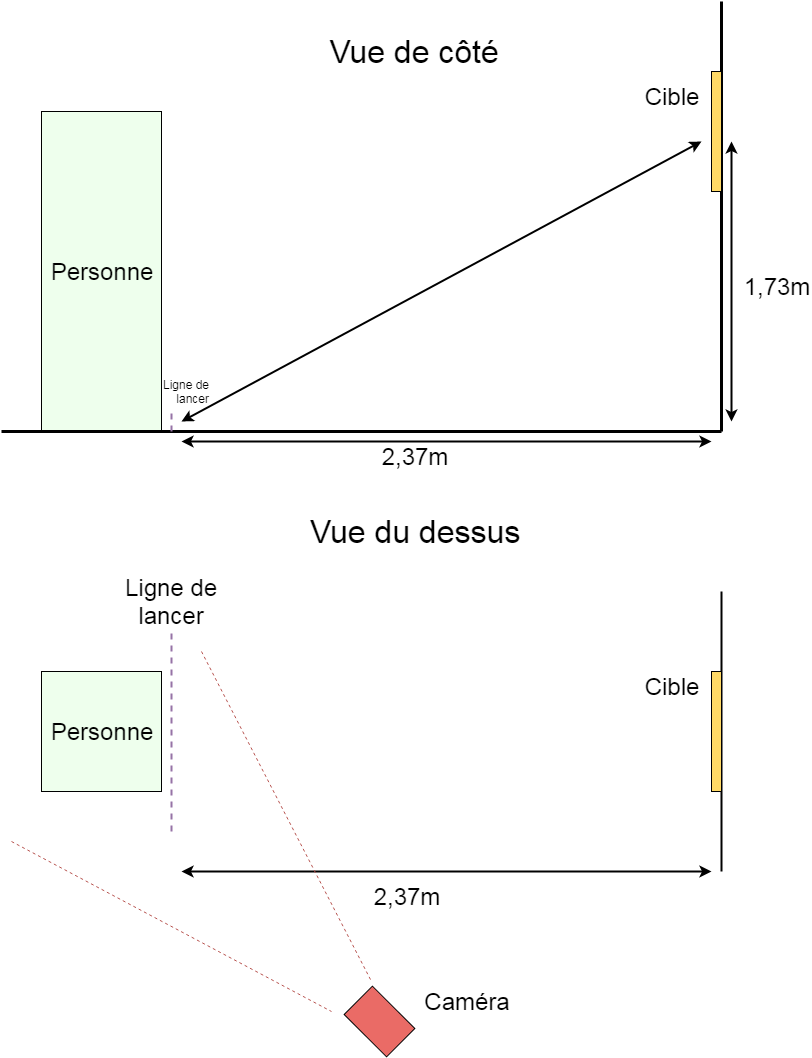
\includegraphics[width=\textwidth]{pictures/Darts_scheme.png}
    \caption{Installation de l'expérimentation.}
    \label{fig:Darts_scheme}
\end{figure}

\subsubsection{Déroulement}
Avant l'expérimentation, un pré-questionnaire était rempli par chaque participant, afin de recueillir sa taille (pour fournir un squelette adapté dans le logiciel de capture de mouvements), le niveau d'expertise autoévalué aux fléchettes (échelle de Likert à 7 réponses), ainsi que toute pratique actuelle d'un sport (voir Annexe 1).

Une fois ce pré-questionnaire rempli, la combinaison de capteurs était installée sur la personne. Les calibrations étaient ensuite effectuées, afin d'étalonner les capteurs (position dans l'espace, espacement des capteurs entre eux, mise à zéro sur le logiciel de capture, etc.) pour que le logiciel puisse adapter la combinaison par rapport aux articulations du squelette 3D.

Chaque participant a reçu comme instruction de viser le centre de la cible à l'aide de fléchettes. La position de lancer étant importante, il a été demandé de se placer perpendiculairement à la marque au sol (Fig. \ref{fig:darts_position}).

\begin{figure}
    \centering
    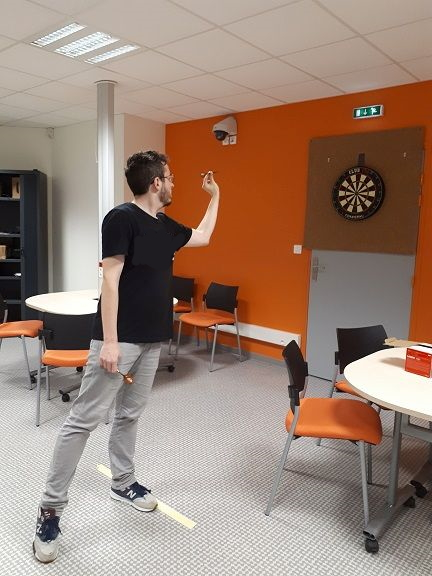
\includegraphics[width=7cm]{pictures/darts_position.jpg}
    \caption{Position latérale imposée aux participants.}
    \label{fig:darts_position}
\end{figure}

Les participants devaient ensuite effectuer neuf lancers de test, non enregistrés. Ces lancers avaient pour buts de permettre à la personne de s'habituer à la combinaison et au lancer, ainsi que de vérifier que le squelette ne présentait pas de problèmes lors du mouvement (dérive des capteurs, mauvais positionnement des capteurs, parties de la combinaison qui ne fonctionnent pas, etc.).

Chaque personne a été affectée à l'un des trois groupes expérimentaux, sans avoir connaissance de cette assignation. Afin d'éviter toute différence de perception, il a été dit à chaque personne que les conseils étaient donnés par le système (même si ce n'était pas le cas pour tous les groupes).

Avant chaque lancer, la personne doit se placer en position de lancer, dire « prêt », puis attendre le signal sonore de départ du logiciel (qui correspond au début de l'enregistrement du mouvement). La personne lance ensuite sa fléchette, puis garde la position finale de son bras jusqu'au deuxième signal sonore (correspondant à l'arrêt de l'enregistrement). L'intervalle de temps entre le premier signal sonore et le lancer varie grandement d'une personne à l'autre ; cependant, l'algorithme de segmentation permet de ne garder que le geste utile pour chaque participant (cf. chapitre \ref{chap:traitement_donnees} section \ref{subsec:MoI}). À chaque lancer, la distance de la fléchette par rapport au centre est relevée (Fig. \ref{fig:target_with_darts_distance}).

\begin{figure}
    \centering
    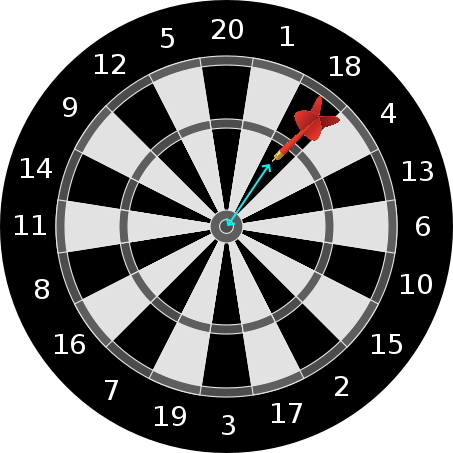
\includegraphics[width=7cm]{pictures/target_with_darts_distance.jpg}
    \caption[Distance relevée entre les fléchettes et le centre de la cible]{En bleu, la distance relevée après chaque lancer de fléchette.}
    \label{fig:target_with_darts_distance}
\end{figure}

Chaque personne a effectué quatre séries de neuf lancers, soit trente-six lancers au total. Au bout d'une série de neuf lancers, les mouvements étaient analysés par le système (indépendamment du fait que les conseils donnés proviennent du système ou non). Pour le premier groupe, les données étaient analysées mais non utilisées par l'expert pour le jugement du geste. Chaque personne recevait alors deux conseils par rapport à son geste. En fonction de son groupe (conseils de l'expert pour le groupe 1, conseils du système pour le groupe 2, conseils de l'expert assisté du système pour le groupe 3). Les conseils donnés (par le système ou l'expert) sont les suivants :
\begin{itemize}
	\item corps penché : « Votre corps et vos épaules ne doivent pas bouger pendant votre lancer. »
	\item lancer type javelot : « Votre main doit toujours rester devant votre corps lorsque vous lancez. »
	\item alignement du bras : « Votre bras doit rester aligné (de la main à l'épaule) lorsque vous lancez. »
	\item mouvement du coude : « Votre coude ne doit pas bouger lors du lancer. »
\end{itemize}

Dans le cas du groupe deux, les conseils sont choisis comme il suit :
\begin{itemize}
	\item La distance entre le centroïde des données de l'apprenant et du cluster de gestes cibles de l'expert est calculée, pour chaque défaut (voir chapitre \ref{chap:traitement_donnees} section \ref{subsec:feedback})
	\item Si deux défauts sont situés soit (i) dans le trapèze reliant les deux clusters, soit (ii) dans le cluster de mauvais gestes de l'expert, les deux conseils correspondant à ces défauts sont donnés
	\item S'il n'y en a qu'un seul, le conseil correspondant au défaut situé dans la zone susmentionnée est donné, puis le conseil correspondant au défaut dont la distance est la plus éloignée du bon cluster est donné
	\item S'il n'y en a aucun, les deux conseils correspondant aux défauts dont les distances sont les plus éloignées du bon cluster sont donnés
\end{itemize}

Dans le cas du groupe 3, une visualisation des données de l'apprenant par rapport à celles de l'expert est proposée (Fig. \ref{fig:feedback_grp_example}). Ainsi, l'expert peut s'appuyer sur cette visualisation pour prendre sa décision. Cette visualisation permet également de compenser un cas particulier : si les données de l'apprenant sont très dispersées, mais centrées autour du cluster de bons mouvements de l'expert, le centroïde des données de l'apprenant sera situé dans le cluster de bons gestes de l'expert. Ainsi, il est possible pour l'expert de repérer ce cas particulier dans le cas où il s'appuie sur le système pour donner ses conseils, et de ne pas considérer que cet aspect des gestes de l'apprenant est réussi. Cependant, dans le cadre de l'expérimentation, l'expert s'est basé sur les valeurs de distance affichées directement, plutôt que sur la visualisation. Il procède comme il suit :
\begin{itemize}
	\item s'il décèle deux défauts, les deux conseils correspondant à ces défauts sont donnés à l'apprenant,
	\item s'il décèle un seul défaut, il donne le conseil correspondant à ce défaut, puis se base sur les valeurs de distance affichées par le système afin de donner le conseil sur le défaut étant le plus éloigné du cluster de bons gestes,
	\item s'il n'arrive pas à déceler de défauts, il se base sur les valeurs de distance affichées par le système, et choisit les deux défauts les plus éloignés du bon cluster.
\end{itemize}


\begin{figure}
    \centering
    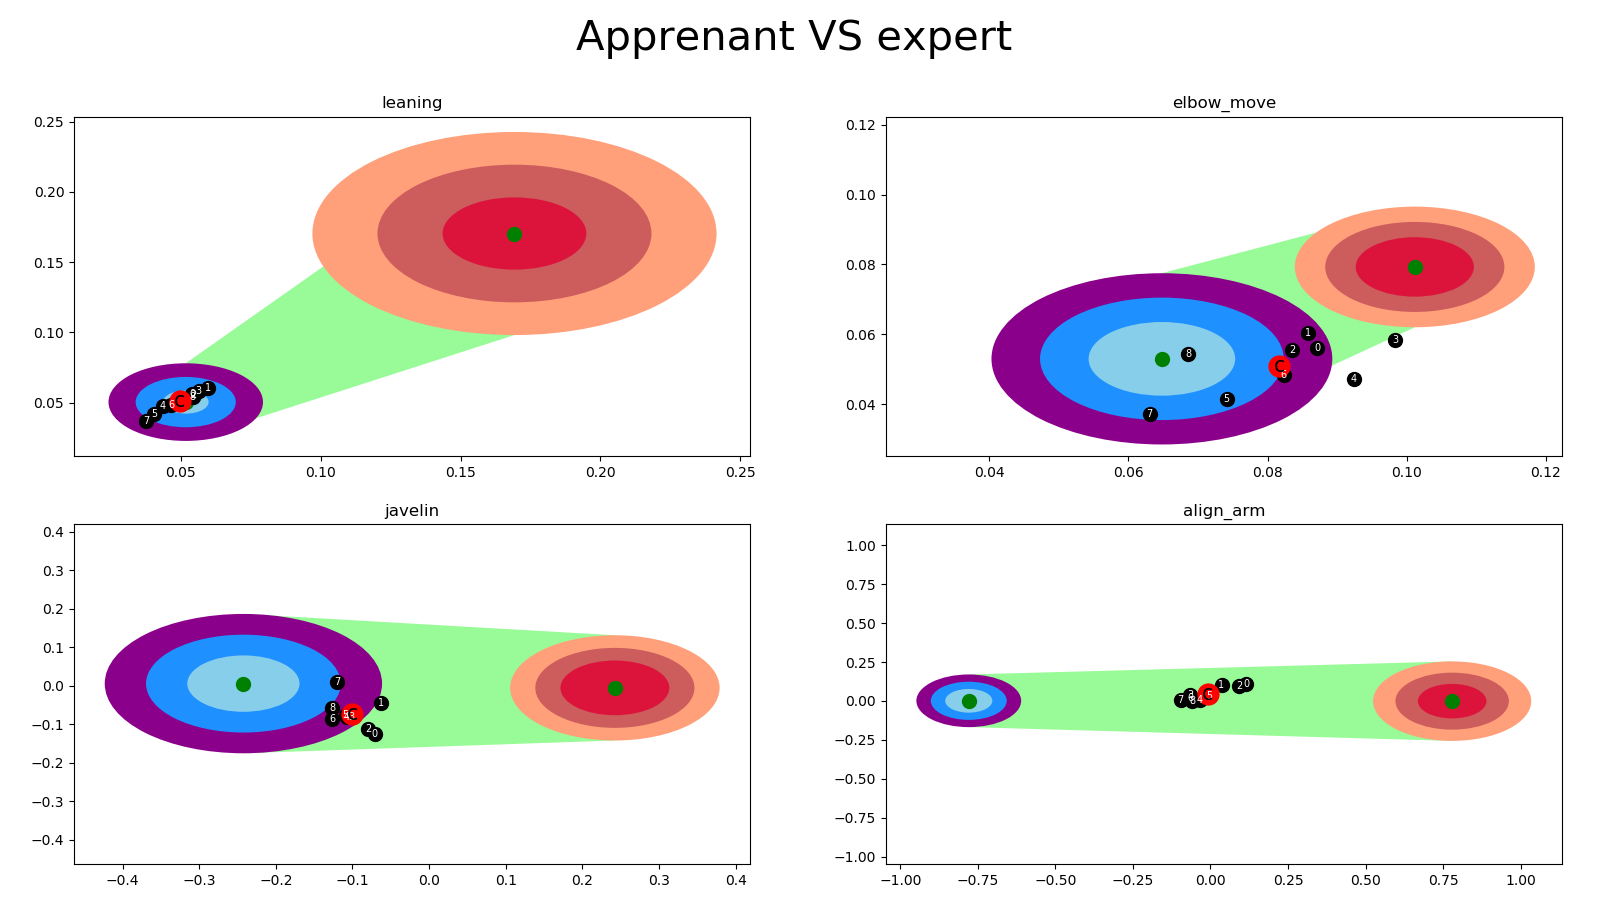
\includegraphics[width=15cm]{pictures/feedback_grp_example.png}
    \caption[Exemple de visualisation à la fin des séries de lancer]{Un exemple de visualisation des données de l'apprenant fournie à l'expert à la fin d'une série de neuf lancers.}
    \label{fig:feedback_grp_example}
\end{figure}

La personne refaisait ensuite 9 lancers, en essayant de tenir compte de ces deux conseils. Il n'y a pas de conseils donnés à la fin de la dernière série.

Une fois l'expérimentation finie, la personne remplit un post-questionnaire (voir Annexe 1). Ce post-questionnaire mesure le ressenti de la personne par rapport à la combinaison, à la progression de son geste et à l'auto-évaluation de sa performance. Les questions sont toutes basées sur l'échelle de Lickert, allant de 1 à 7. Les questions portent sur :
\begin{itemize}
	\item le niveau d'aisance avec le matériel,
	\item le niveau de stress de l'apprenant lors de l'expérimentation,
	\item le niveau de compréhension des instructions reçues,
	\item l'intérêt ressenti des conseils donnés,
	\item l'auto-évaluation de la performance sur toute l'expérimentation,
	\item l'auto-évaluation de la progression de la performance sur toute l'expérimentation,
	\item l'auto-évaluation de la qualité du geste sur toute l'expérimentation,
	\item l'auto-évaluation de la progression de la qualité du geste sur toute l'expérimentation,
	\item l'expression libre (remarques diverses).
\end{itemize}


\subsubsection{Métriques calculées sur le clustering des données de l'expert}
L'algorithme utilisé afin de regrouper les données de l'expert est un \textit{k-means}, avec $k = 2$. Les métriques d'ASS et d'ARI ont été calculées sur les regroupements obtenus (voir tableau \ref{tab:ass_ari_darts}).

\begin{table}[h]
\centering
\begin{tabular}{c|c|c}
& Silhouette Score & Adjusted Rand Index\\\hline
Leaning & 0.85 & 1\\
elbow move & 0.58 & 0.47\\
javelin & 0.79 & 1\\
align arm & 0.53 & 1\\
\end{tabular}
\caption{Valeurs de l'Average Silhouette Score et de l'Adjusted Rand Index pour les données de l'expert sur les quatre défauts.}
\label{tab:ass_ari_darts}
\end{table}

Les valeurs pour l'\textit{ASS} sont supérieures ou égales à celles obtenues pour les deux expérimentations précédentes, suggérant une bonne (voire très bonne) séparation des données. L'hypothèse \textbf{H3} est validée dans le contexte de cette expérimentation. Les valeurs pour l'\textit{ARI} suggèrent que le regroupement des données d'un défaut (mouvement du coude) ne correspond pas exactement à la vérité terrain relevée. Cela implique que certaines des données de l'expert ne sont pas séparables de manière fidèle à la vérité terrain à l'aide des descripteurs utilisés. Cela peut s'expliquer soit par (i) un mauvais choix de descripteurs, soit par (ii) des mouvements de l'expert où la différence entre le geste correct et le défaut n'est pas assez prononcée. Dans ces cas, le clustering permet d'obtenir un regroupement des données selon leur similitude, plutôt que l'étiquetage relevé.

\subsection{Résultats}
Les résultats de l'expérimentation ont été analysés sous deux angles : l'amélioration de l'objectif du mouvement (c'est-à-dire la distance des fléchettes par rapport au centre de la cible) et l'amélioration des propriétés du mouvement de l'apprenant (c'est-à-dire le rapprochement du centroïde de l'apprenant du cluster de l'expert pour chaque défaut). L'analyse a été réalisée sous deux aspects : l'analyse intergroupes pour chaque jeu de lancers, et l'analyse intragroupe, sur les quatre jeux pour chaque groupe. L'objectif est double : (i) vérifier qu'il y a une amélioration significative du geste (au sens des tests statistiques effectués) au cours de l'expérimentation, que le système soit utilisé ou non et (ii) vérifier l'existence d'une différence significative (au sens des tests statistiques effectués) de l'amélioration du geste en fonction de l'utilisation faite du système : expert assisté, système seul ou sans système.

\subsubsection{Tests utilisés}

Deux tests de normalité sont utilisés pour évaluer si la distribution des données suit une loi normale : le test de Shapiro-Wilk, et le test d'Agostino-Pearson. Plus précisément, le test de Shapiro-Wilk teste l'hypothèse nulle selon laquelle la population est normalement distribuée. Bien que ce test soit parfois recommandé pour tester la normalité de données \parencite{Thode2002Tfn} et soit très largement utilisé, il n'est que peu efficace lorsque plusieurs données ont la même valeur. Ainsi, le test d'Agostino-Pearson est également utilisé, permettant de pallier ce problème \parencite{DAgostino1990ASf}.
Le niveau alpha de comparaison utilisé est $0.05$ dans les deux cas.

La distribution de la population selon une loi normale permet d'utiliser des tests paramétriques, plus précis que leurs contreparties non-paramétriques (qui ne font aucune hypothèse sur la distribution des données). Dans le cas des données analysées, la distribution ne suit pas systématiquement une loi normale. Les résultats des tests paramétriques et non-paramétriques sont présentés dans les tableaux, mais seuls les tests pertinents au regard de la distribution des données sont analysés.

Pour l'analyse intergroupe, 15 personnes différentes pour chaque groupe ont réalisé l'expérimentation. Nous supposerons donc que les échantillons de données résultants de l'activité humaine, dans le contexte de cette expérimentation, sont indépendants entre les groupes.

\paragraph{Tests pour les résultats intergroupe}
Dans le cas d'une distribution normale de la population, où l'on compare deux échantillons issus de populations différentes, les tests utilisés sont des tests paramétriques. Le test choisi ici est l'ANOVA (\textit{\textbf{AN}alysis \textbf{O}f \textbf{VA}riance}). Son objectif est de déterminer si les distributions suivent une même loi normale (hypothèse nulle) ou si au moins une des moyennes des distributions est différente de celles des autres échantillons (hypothèse alternative). Si l'hypothèse nulle est vérifiée, l'homogénéité des variances des groupes est alors vérifiée à l'aide du test de Levene. Dans ce test, l'hypothèse nulle stipule que les variances de population sont égales. Enfin, un test de Student paire-à-paire est effectué, afin d'identifier les différences significatives entre les groupes pris deux-à-deux.\\

Dans le cas où la distribution de la population ne suit pas une loi normale, les tests non-paramétriques sont utilisés. Ces tests nécessitent plus de données que leur contrepartie paramétrique. Le premier test utilisé est celui de Kruskal-Wallis ; il est la contrepartie non-paramétrique du test d'ANOVA. L'hypothèse nulle est que les médianes de chaque groupe sont égales, l'hypothèse alternative étant qu'au moins une médiane d'un groupe est différente d'au moins l'une de celles des autres groupes. Si l'hypothèse nulle est vérifiée, un test de Wilcoxon-Mann-Whitney est utilisé, afin de tester si les distributions sont égales (hypothèse nulle).


Pour l'analyse intragroupe, dans chacun des groupes pris indépendamment, les 15 mêmes personnes réalisent chacun des 4 jeux de lancers à la suite. Nous supposerons donc que les échantillons de données résultants de l'activité humaine, dans le contexte de cette expérimentation, sont dépendants entre les jeux.

\paragraph{Tests pour les résultats intragroupes}
Dans le cas où la distribution de la population suit une loi normale, le test de Student sur deux échantillons est utilisé. L'hypothèse nulle de ce test stipule que la moyenne des deux populations est égale.\\

Dans le cas où la distribution de la population ne suit pas une loi normale, le test non-paramétrique utilisé est le test des rangs signés de Wilcoxon (la contrepartie non-paramétrique du test de Student sur deux échantillons). L'hypothèse nulle de ce test est que la médiane de deux échantillons est égale.
\vspace{0.5cm}


Dans tous les cas considérés, il faut noter que le rejet ou la validation de l'hypothèse nulle n'est pas une preuve formelle que les résultats sont reproductibles et valides \parencite{Halsey2015Tfp}. Lorsque l'hypothèse nulle est rejetée, le résultat est considéré comme significatif et n'est pas dû à un phénomène aléatoire. Cependant, ce n'est pas une preuve formelle que la différence significative obtenue entre les échantillons soit liée à leur condition expérimentale respective identifiée par le chercheur. L'interprétation des résultats significatifs obtenus en comparant les différences dans les conditions expérimentales doit être menée avec une grande prudence et se limiter au cadre expérimental défini. La reproductibilité des résultats ne peut être alors qu'envisagée dans les limites du cadre, tandis que la généralisation peut être uniquement supposée. À l'inverse, lorsque l'hypothèse nulle est validée, il n'est généralement pas utile de pousser plus loin l'interprétation des résultats obtenus.

Cette partie ne présentera que les résultats pertinents au regard des tests considérés. Les tableaux complets d'analyse sont disponibles dans l'annexe 2.

Pour chaque analyse, les données sont affichées sous forme de diagrammes en boîte. Ces diagrammes, également appelés boîtes à moustaches, permettent de visualiser :
\begin{itemize}[label=$-$]
	\item la moyenne (losange noir),
	\item la médiane (barre noire),
	\item les valeurs du premier et troisième quartile (l'extrémité basse et haute des boîtes, respectivement),
	\item la différence entre $q_3$ et $q_1$ est appelée écart interquartile, et est défini par la différence $q_3 - q_1$,
	\item les limites (moustaches) représentées respectivement par les points les plus proches de $q_1 - \frac{q_3 - q_1}{1.5}$ et $q_3 + \frac{q_3 - q_1}{1.5}$,
	\item la dispersion, représentée par l'écart entre les limites (moustaches),
	\item les données aberrantes, situées en deçà ou au-delà des limites (points rouges).
\end{itemize}


\subsubsection{Distance des fléchettes par rapport au centre de la cible}

Le tableau \ref{tab:moy_std_precision} présente les moyennes et les écarts-types des distances des fléchettes par rapport au centre de la cible lors des lancers des participants. On remarque une dégradation systématique de la moyenne, ainsi que de l'écart-type, entre le jeu 1 et le jeu 2. Ces valeurs tendent à diminuer pour les jeux suivants, sauf dans le cas du groupe 3, ou la valeur augmente entre le jeu 2 et le jeu 3, puis diminue ensuite. La différence entre le jeu 1 et le jeu 4 montre que ces valeurs se rapprochent des valeurs initiales. Ces résultats suggèrent que les premiers conseils donnés entraînent une perte de précision du geste, puis que les participants réussissent à améliorer la précision de leurs lancers.

\begin{table}[]
\small
\makebox[\textwidth][c]{
\begin{tabular}{l|llllllll}
 & \multicolumn{2}{c}{Jeu 1} & \multicolumn{2}{c}{Jeu 2} & \multicolumn{2}{c}{Jeu 3} & \multicolumn{2}{c}{Jeu 4} \\
 & Moyenne & Écart-Type & Moyenne & Écart-Type & Moyenne & Écart-Type & Moyenne & Écart-Type \\\hline
Groupe 1 & 10.1481 & 3.8336 & 14.4170 & 5.4708 & 10.9926 & 3.2721 & 10.2481 & 3.5990 \\
Groupe 2 & 10.2481 & 3.6957 & 13.5741 & 6.4499 & 11.9674 & 4.6060 & 10.9296 & 3.6617 \\
Groupe 3 & 9.7393 & 2.3020 & 11.9667 & 4.0647 & 12.6889 & 5.7258 & 11.0074 & 5.4516
\end{tabular}}
\caption{Moyennes et écarts-types des données des apprenants (distance au centre de la cible).}
\label{tab:moy_std_precision}
\end{table}

Les résultats intergroupes sont présentés dans la figure \ref{fig:Precision_All_data_intergroupe}. Pour chaque jeu (un jeu par graphique), les données des trois groupes sont présentées en parallèle. La figure \ref{fig:Precision_All_data_intragroupe} montre la progression de la précision en intra-groupe pour chaque groupe (un groupe par graphique).

Sur la figure \ref{fig:Precision_All_data_intragroupe}, on peut observer une augmentation systématique de la valeur de la médiane ainsi que de la dispersion des données entre le jeu 1 et le jeu 2 pour tous les groupes, correspondant à une augmentation de la distance par rapport au centre. S'en suit une réduction de la dispersion des valeurs pour les jeux suivants (sauf pour le jeu 4 du groupe 3), suggérant ainsi une précision des lancers en hausse. Cependant, la précision ne revient pas à une valeur inférieure ou égale à celle du premier jeu (en terme de médiane, moyenne et précision). Cette tendance est la plus visible pour le groupe 1. Des résultats significatifs ont été obtenus entre les jeux 1 et 2 et les jeux 2 et 4 pour chaque groupe (tableau \ref{tab:precision_intra}), montrant d'une part une dégradation systématique de la distance par rapport au centre de la cible à la suite des premiers conseils donnés, quel que soit le groupe considéré, et une amélioration progressive de la précision du lancer au fil de l'expérimentation. Des résultats significatifs ont également été obtenus entre le jeu 1 et le jeu 3 pour les groupes 2 et 3, le jeu 2 et le jeu 3 pour le groupe 1 et le jeu 3 et le jeu 4 pour le groupe 3. Cette dégradation semble correspondre au « désapprentissage » du geste initial au profit de l'apprentissage du geste cible. On constate la présence de données aberrantes sur les trois groupes, dont au moins une persistante sur les quatre jeux pour les groupes 2 et 3. Il y a plus de données aberrantes pour le groupe 3 (entre une et trois, selon le jeu considéré), malgré le fait que ce groupe soit celui présentant les meilleures valeurs de médianes, écart interquartile et dispersion.


Pour l'analyse intergroupe (figure \ref{fig:Precision_All_data_intergroupe}), on observe que le groupe 3 est celui dont l'écart interquartile est le plus faible sur tous les jeux sauf le quatrième (groupe 1), tout en ayant le plus de données aberrantes. Le groupe 1 est celui ayant la médiane la plus basse sur tous les jeux, sauf le deuxième (groupe 3). Dans les deux cas, les résultats ne présentent pas de différences significatives (tableau \ref{tab:precision_inter}).
\afterpage{
\begin{landscape}
\begin{table}[]
\centering
\begin{tabular}{ll|ccccc|cccc}
    &  & \multicolumn{5}{c|}{Wilcoxon Signed-Rank ($p < 0.05$)} & \multicolumn{4}{c}{T Test ($p < 0.05$)} \\ \cline{3-11}
    &  & \multicolumn{2}{c|}{One tail} & \multicolumn{2}{c}{Two tails} &  & \multirow{2}{*}{One tail} & \multirow{2}{*}{Two tails} & \multirow{2}{*}{t} & \multirow{2}{*}{df} \\ \cline{3-7}
    &  & p-norm & p-exact & p-norm & p-exact & T &  &  &  &  \\ \hline
 \multirow{3}{*}{Jeu 1-2} & G1 & \cellcolor{green!25} 0.0057 & \cellcolor{green!25} 0.0042 & \cellcolor{green!25} 0.0115 & \cellcolor{green!25} 0.0084 & 15 &  &  &  &  \\
 & G2 & \cellcolor{green!25} 0.0021 & \cellcolor{green!25} 0.0010 & \cellcolor{green!25} 0.0041 & \cellcolor{green!25} 0.0020 & 9 &  &  &  &  \\
 & G3 & \cellcolor{green!25} 0.0038 & \cellcolor{green!25} 0.0021 & \cellcolor{green!25} 0.0076 & \cellcolor{green!25} 0.0043 & 12.5 &  &  &  &  \\ \hline
\multirow{3}{*}{Jeu 2-3} & G1 & \cellcolor{green!25} 0.0049 & \cellcolor{green!25} 0.0034 & \cellcolor{green!25} 0.0098 & \cellcolor{green!25} 0.0067 & 14 &  &  &  &  \\
 & G2 & 0.1006 & 0.1039 & 0.2013 & 0.2078 & 37 &  &  &  &  \\
 & G3 & 0.5 & 0.4890 & 1 & 0.9780 & 59.5 &  &  &  &  \\ \hline
\multirow{3}{*}{Jeu 3-4} & G1 &  &  &  &  &  & 0.1514 & 0.3028 & 1.0698 & 14 \\
 & G2 & 0.1221 & 0.1262 & 0.2443 & 0.2524 & 39 & 0.1439 & 0.2877 & 1.1052 & 14 \\
 & G3 & \cellcolor{green!25} 0.0144 & \cellcolor{green!25} 0.0128 & \cellcolor{green!25} 0.0288 & \cellcolor{green!25} 0.0256 & 21 &  &  &  &  \\ \hline
\multirow{3}{*}{Jeu 1-3} & G1 & 0.1601 & 0.1651 & 0.3202 & 0.3303 & 42 &  &  &  &  \\
 & G2 & 0.1110 & 0.1146 & 0.2220 & 0.2293 & 38 &  &  &  &  \\
 & G3 & \cellcolor{green!25} 0.01659 & \cellcolor{green!25} 0.0151 & \cellcolor{green!25} 0.0332 & \cellcolor{green!25} 0.0301 & 22 &  &  &  &  \\ \hline
\multirow{3}{*}{Jeu 2-4} & G1 & \cellcolor{green!25} 0.0005 & \cellcolor{green!25} $9.1553e^{-5}$ & \cellcolor{green!25} 0.0011 & \cellcolor{green!25} 0.0002 & 2 &  &  &  &  \\
 & G2 & \cellcolor{green!25} 0.0073 & \cellcolor{green!25} 0.0051 & \cellcolor{green!25} 0.0146 & \cellcolor{green!25} 0.0102 & 16.5 &  &  &  &  \\
 & G3 & \cellcolor{green!25} 0.0250 & \cellcolor{green!25} 0.0240 & \cellcolor{green!25} 0.0500 & \cellcolor{green!25} 0.0479 & 25 &  &  &  &  \\ \hline
\multirow{3}{*}{Jeu 1-4} & G1 & 0.4660 & 0.4670 & 0.9321 & 0.9341 & 58 &  &  &  &  \\
 & G2 & 0.0864 & 0.0844 & 0.1728 & 0.1688 & 35.5 &  &  &  &  \\
 & G3 & 0.2051 & 0.2106 & 0.4102 & 0.4212 & 45 &  &  &  &
\end{tabular}
\caption{Résultats des tests statistiques en intragroupe (distance par rapport au centre).}
\label{tab:precision_intra}
\end{table}
\end{landscape}}

\begin{table}[]
\centering
\begin{tabular}{lr|cccc}
 &  & Jeu 1 & Jeu 2 & Jeu 3 & Jeu 4 \\\hline
\multirow{2}{*}{ANOVA} &  &  &  &  &  \\
 &  &  &  &  &  \\\hline
\multirow{3}{*}{Pairwise T-test} & & & & & \\
 & & & & &  \\
 & & & & &  \\\hline
\multirow{3}{*}{Kruskal-Wallis ($p < 0.05$)} & Chi-square & 0.1875 & 1.8023 & 0.4432 & 0.3937 \\
 & p & 0.9907 & 0.4061 & 0.8012 & 0.8213 \\
 & df & 2 & 2 & 2 & 2 \\\hline
\multirow{3}{*}{Pairwise Mann-Whitney} & & & & & \\
 & & & & & \\
 & & & & &
\end{tabular}
\caption{Résultats des tests statistiques en intergroupe (distance par rapport au centre).}
\label{tab:precision_inter}
\end{table}


\begin{figure}%[H]
	\centering
	\makebox[\textwidth][c]{
    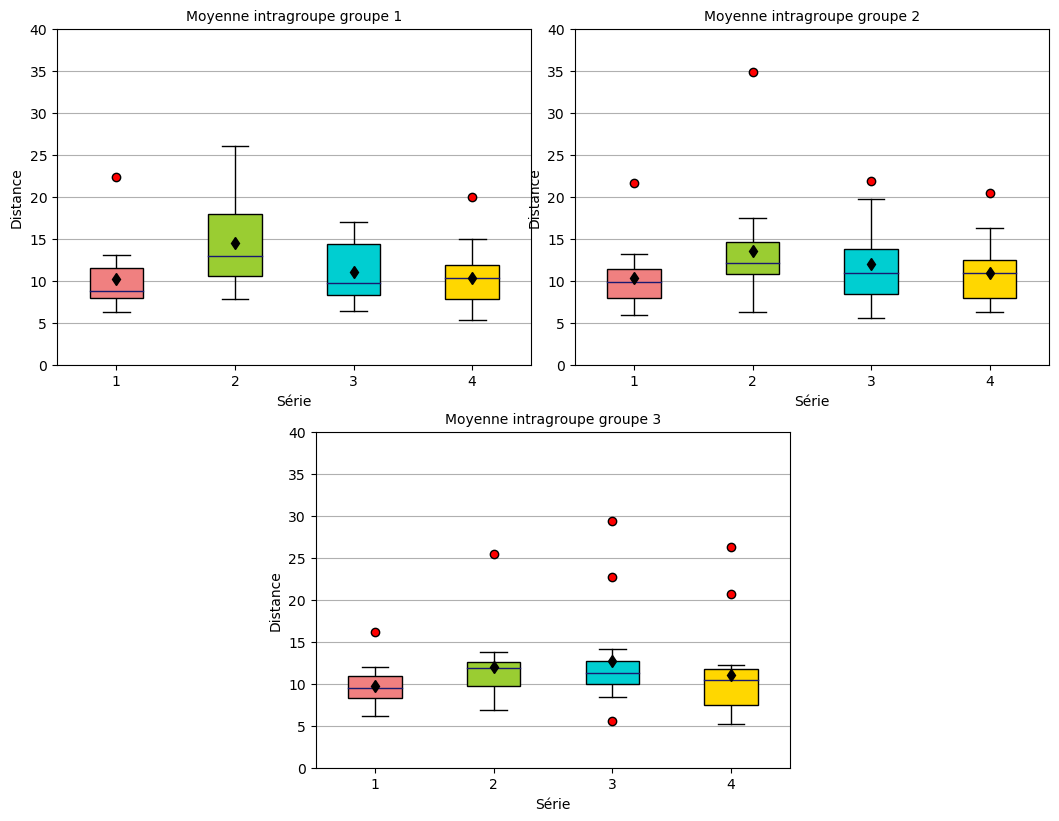
\includegraphics[width=15cm]{expe_results/Precision_All_data_intragroupe.png}}
    \caption[Moyennes des distances des fléchettes par rapport au centre en intra-groupe]{Moyennes des distances des fléchettes par rapport au centre de la cible en intra-groupe.}
    \label{fig:Precision_All_data_intragroupe}
\end{figure}


\begin{figure}%[H]
	\centering
	\makebox[\textwidth][c]{
    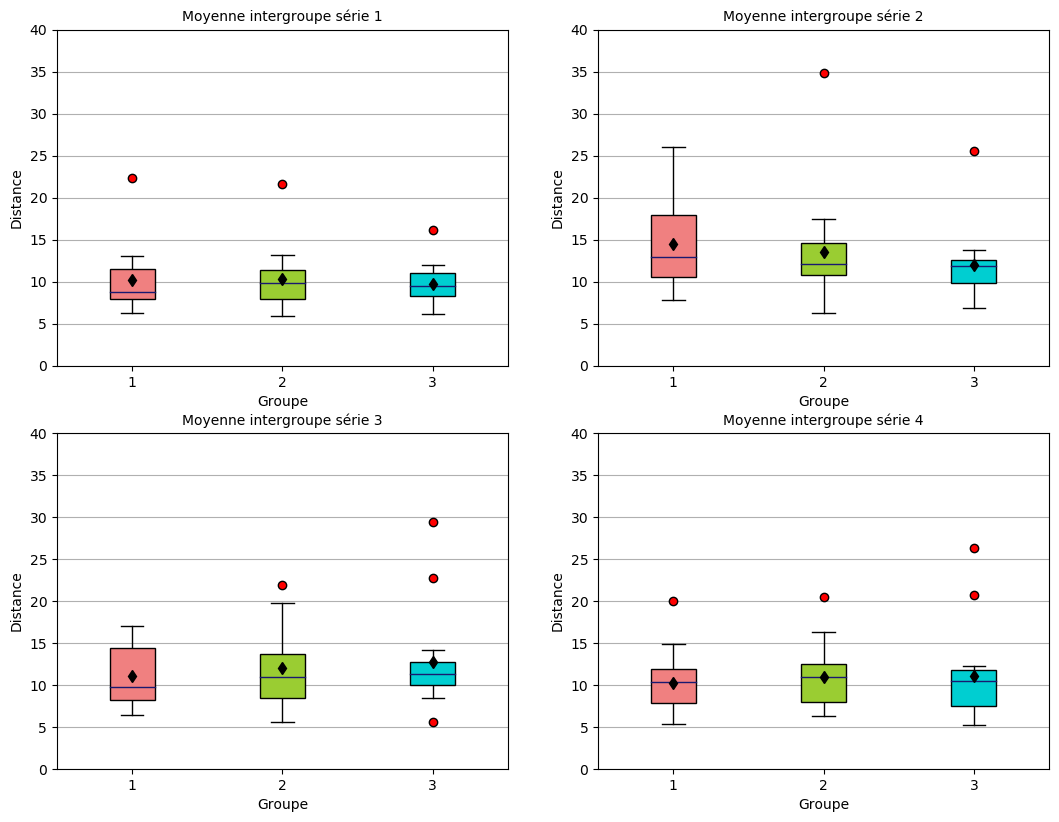
\includegraphics[width=15cm]{expe_results/Precision_All_data_intergroupe.png}}
    \caption[Moyennes des distances des fléchettes par rapport au centre en inter-groupe]{Moyennes des distances des fléchettes par rapport au centre de la cible en inter-groupe.}
    \label{fig:Precision_All_data_intergroupe}
\end{figure}



\subsubsection{Amélioration des défauts du mouvement}

Le tableau \ref{tab:advices_freq} montre la fréquence à laquelle sont donnés les conseils entre chaque jeu. On remarque qu'après le premier jeu, le défaut du corps penché est plus détecté que les autres, à l'inverse du défaut de l'alignement du bras. Cela peut s'expliquer par la facilité d'observation du défaut du corps penché par l'expert, à l'inverse de l'alignement du bras à cause de la position d'observation (visible sur la figure \Ref{fig:Darts_scheme}). À l'inverse, pour les conseils donnés à la fin du jeu 3, le défaut du corps penché est moins donné, car souvent corrigé dès les premiers jeux.

Le tableau \ref{tab:advices_groupes_freq} présente la fréquence des conseils donnés pour chaque groupe, entre chaque jeu et pour chaque groupe. Ainsi, on peut constater que le défaut du corps penché est très souvent détecté comme étant le défaut à corriger en premier, quel que soit le groupe considéré. Ce défaut est en fait une caractéristique des lancers de manière générale : se pencher lors d'un lancer permet d'imprimer plus de force au projectile. Pour le groupe 1, le conseil le plus donné est celui du mouvement du coude. Ce défaut est facilement observable lors du geste d'un apprenant, et donc l'expert tend à se concentrer sur ce défaut tant qu'il n'estime pas le mouvement satisfaisant. À l'inverse, le défaut du lancer de type javelot est rarement considéré par l'expert. En effet, il est plus difficilement observable que les autres dans le contexte de cette expérimentation. Le système seul tend à donner les conseils sur les mêmes deux défauts pour les deux premiers jeux, à savoir le lancer de type javelot et le corps penché. Pour le troisième jeu, la fréquence des conseils s'harmonise, suggérant ainsi une stabilisation au niveau de tous les défauts (sans pour autant systématiquement atteindre une correction acceptable). Enfin, on remarque que le groupe 3 est celui présentant la répartition de conseils la plus homogène.

%\begin{table}[]
%\begin{tabular}{l|lll}
%           & jeu 1-2 & jeu 2-3 & jeu 3-4 \\\hline
%align arm  & 8       & 21      & 24      \\
%elbow move & 24      & 26      & 27      \\
%javelin    & 24      & 22      & 22      \\
%leaning    & 34      & 21      & 17
%\end{tabular}
%\caption{Fréquence des conseils donnés (en pourcentage) en fonction des jeux.}
%\label{tab:advices_freq_base}
%\end{table}
%
%\begin{table}[]
%\begin{tabular}{llll}
%           & jeu 1-2 & jeu 2-3 & jeu 3-4 \\
%align arm  & 9       & 23      & 27      \\
%elbow move & 27      & 29      & 30      \\
%javelin    & 26      & 25      & 24      \\
%leaning    & 38      & 23      & 19
%\end{tabular}
%\caption{Fréquence des conseils donnés (en pourcentage) en fonction des jeux.}
%\label{tab:advices_freq_perc}
%\end{table}

\begin{table}%[H]
\centering
\begin{tabular}{l|lll}
           & jeu 1-2 & jeu 2-3 & jeu 3-4 \\\hline
align arm  & 0.09      & 0.23      & 0.27      \\
elbow move & 0.27      & 0.29      & 0.30      \\
javelin    & 0.26      & 0.25      & 0.24      \\
leaning    & 0.38      & 0.23      & 0.19
\end{tabular}
\caption{Fréquences des conseils donnés en fonction des jeux.}
\label{tab:advices_freq}
\end{table}

%\begin{table}[]
%\begin{tabular}{ll|llll}
%                    &         & align arm & elbow move & javelin & leaning \\\hline
%\multirow{3}{*}{G1} & Jeu 1-2 & 3         & 13         & 3       & 11      \\
%                    & Jeu 2-3 & 10        & 10         & 6       & 4       \\
%                    & Jeu 3-4 & 11        & 12         & 2       & 5       \\\hline
%\multirow{3}{*}{G2} & Jeu 1-2 & 2         & 3          & 14      & 11      \\
%                    & Jeu 2-3 & 4         & 5          & 10      & 11      \\
%                    & Jeu 3-4 & 6         & 6          & 11      & 7       \\\hline
%\multirow{3}{*}{G3} & Jeu 1-2 & 3         & 8          & 7       & 12      \\
%                    & Jeu 2-3 & 7         & 11         & 6       & 6       \\
%                    & Jeu 3-4 & 7         & 9          & 9       & 5
%\end{tabular}
%\caption{Fréquence des conseils donnés pour chaque groupe, en fonction des jeux.}
%\label{tab:advices_groupes_base}
%\end{table}
%
%\begin{table}[]
%\begin{tabular}{llllll}
%                    &         & align arm & elbow move & javelin & leaning \\
%\multirow{3}{*}{G1} & Jeu 1-2 & 10        & 43         & 10      & 37      \\
%                    & Jeu 2-3 & 33        & 33         & 20      & 14      \\
%                    & Jeu 3-4 & 37        & 40         & 6       & 17      \\
%\multirow{3}{*}{G2} & Jeu 1-2 & 6         & 10         & 47      & 37      \\
%                    & Jeu 2-3 & 13        & 16         & 33      & 37      \\
%                    & Jeu 3-4 & 20        & 20         & 37      & 23      \\
%\multirow{3}{*}{G3} & Jeu 1-2 & 10        & 27         & 23      & 40      \\
%                    & Jeu 2-3 & 23        & 37         & 20      & 20      \\
%                    & Jeu 3-4 & 23        & 30         & 30      & 17
%\end{tabular}
%\caption{Fréquence des conseils donnés pour chaque groupe, en fonction des jeux.}
%\label{tab:advices_groupes_perc}
%\end{table}

\begin{table}%[H]
\centering
\begin{tabular}{ll|llll}
                    &         & align arm & elbow move & javelin & leaning \\\hline
\multirow{3}{*}{G1} & Jeu 1-2 & 0.10      & 0.43       & 0.10    & 0.37    \\
                    & Jeu 2-3 & 0.33      & 0.33       & 0.20    & 0.14    \\
                    & Jeu 3-4 & 0.37      & 0.40       & 0.06    & 0.17    \\\hline
\multirow{3}{*}{G2} & Jeu 1-2 & 0.06      & 0.10       & 0.47    & 0.37    \\
                    & Jeu 2-3 & 0.13      & 0.16       & 0.33    & 0.37    \\
                    & Jeu 3-4 & 0.20      & 0.20       & 0.37    & 0.23    \\\hline
\multirow{3}{*}{G3} & Jeu 1-2 & 0.10      & 0.27       & 0.23    & 0.40    \\
                    & Jeu 2-3 & 0.23      & 0.37       & 0.20    & 0.20    \\
                    & Jeu 3-4 & 0.23      & 0.30       & 0.30    & 0.17
\end{tabular}
\caption{Fréquences des conseils donnés pour chaque groupe, en fonction des jeux.}
\label{tab:advices_groupes_freq}
\end{table}

\paragraph{Align arm}
Le tableau \ref{tab:moy_std_align_arm} présente les moyennes et les écarts-types de la distance des données des participants par rapport au centroïde du cluster de bons gestes de l'expert, pour le défaut de l'alignement du bras. On remarque une amélioration des moyennes pour le groupe 1 entre les jeux 1 et 2, suivi d'une dégradation de ces valeurs. L'écart-type suit les mêmes tendances pour les trois groupes, suggérant ainsi que la correction des autres défauts se fait au détriment de l'alignement du bras, ou que le défaut d'alignement du bras n'est détecté qu'entre le jeu 1 et le 2, puis non-détecté par la suite.

\begin{table}[H]
\small
\makebox[\textwidth][c]{
\begin{tabular}{l|llllllll}
 & Jeu 1 &  & Jeu 2 &  & Jeu 3 &  & Jeu 4 &  \\
 & Moyenne & Écart-Type & Moyenne & Écart-Type & Moyenne & Écart-Type & Moyenne & Écart-Type \\\hline
Groupe 1 & 0.0836 & 0.0548 & 0.0547 & 0.0486 & 0.0656 & 0.0439 & 0.0727 & 0.0496 \\
Groupe 2 & 0.0836 & 0.0556 & 0.0567 & 0.0375 & 0.0497 & 0.0452 & 0.0490 & 0.0391 \\
Groupe 3 & 0.0677 & 0.0342 & 0.0606 & 0.0283 & 0.0578 & 0.0316 & 0.0592 & 0.0356
\end{tabular}}
\caption{Moyennes et écarts-types des données des apprenants (alignement du bras).}
\label{tab:moy_std_align_arm}
\end{table}

Les résultats intergroupes pour le défaut d'alignement du bras sont présentés sur la figure \ref{fig:Align_arm_All_data_intergroupe}, et les résultats en intragroupe sont présentés sur la figure \ref{fig:Align_arm_All_data_intragroupe}.

Pour le groupe 1, la figure \ref{fig:Align_arm_All_data_intragroupe} montre que le défaut se réduit au jeu 2, mais reprend ensuite de l'ampleur dans les jeux suivants (et dépasse au final les valeurs initiales), tant au niveau de l'écart interquartile que de la valeur de la médiane. Le défaut se réduit également pour le groupe 2, sauf pour le 4ème jeu où la valeur de la médiane et l'écart interquartile augmentent. Enfin, les valeurs du groupe 3 sont stables pour la valeur de la médiane, avec une dégradation de la valeur de la médiane sur le jeu 2, suivie par une amélioration de cette valeur, un écart interquartile qui reste sensiblement le même sur les quatre jeux et une dispersion des données variant grandement entre chaque jeu. Aucun résultat significatif n'a été trouvé pour le groupe 3, ce qui rend difficile l'explication de la rapide stabilité de ce défaut pour ce groupe. Les résultats sont significatifs pour le groupe 2 entre les jeux 1-2, 1-3 et 1-4 (table \ref{tab:align_arm_intra}), et pour le groupe 1 entre les jeux 1-2, mais le conseil n'est que peu donné, suggérant ainsi que le défaut est corrigé par les apprenants au travers d'un autre conseil. Il y a, pour chaque groupe, au moins une donnée aberrante.


En analyse intergroupe (figure \ref{fig:Align_arm_All_data_intergroupe}), les écarts interquartiles les plus faibles sont obtenus par les groupes 1 et 3 sur les deux premiers jeux, puis par les groupes 2 et 3 pour les deux derniers jeux. Les moyennes sont également sensiblement meilleures pour ces mêmes groupes. La dispersion est cependant meilleure pour le groupe 1 lors des deux premiers jeux. Aucun de ces résultats ne présente de différences significatives (table \ref{tab:align_arm_inter}).

\afterpage{
\begin{landscape}
\begin{table}[]
\centering
\begin{tabular}{ll|ccccc|cccc}
    &  & \multicolumn{5}{c|}{Wilcoxon Signed-Rank ($p < 0.05$)} & \multicolumn{4}{c}{T Test ($p < 0.05$)} \\ \cline{3-11}
    &  & \multicolumn{2}{c|}{One tail} & \multicolumn{2}{c}{Two tails} &  & \multirow{2}{*}{One tail} & \multirow{2}{*}{Two tails} & \multirow{2}{*}{t} & \multirow{2}{*}{df} \\ \cline{3-7}
    &  & p-norm & p-exact & p-norm & p-exact & T &  &  &  &  \\ \hline
   \multirow{3}{*}{Jeu 1-2} & G1 & \cellcolor{green!25} 0.0035 & \cellcolor{green!25} 0.0021 & \cellcolor{green!25} 0.0070 & \cellcolor{green!25} 0.0043 & 12 &  &  &  &  \\
    & G2 & \cellcolor{green!25} 0.0285 & \cellcolor{green!25} 0.0277 & 0.0571 & 0.0553 & 26 &  &  &  &  \\
    & G3 & 0.2389 & 0.2443 & 0.4777 & 0.4887 & 47 &  &  &  &  \\ \hline
   \multirow{3}{*}{Jeu 2-3} & G1 & 0.1110 & 0.1146 & 0.2220 & 0.2293 & 38 &  &  &  &  \\
    & G2 & 0.2568 & 0.2622 & 0.5136 & 0.5245 & 48 &  &  &  &  \\
    & G3 &  &  &  &  &  & 0.3905 & 0.7809 & 0.2835 & 14 \\ \hline
   \multirow{3}{*}{Jeu 3-4} & G1 & 0.2216 & 0.2271 & 0.4432 & 0.4543 & 46 &  &  &  &  \\
    & G2 & 0.4660 & 0.4670 & 0.9321 & 0.9341 & 58 &  &  &  &  \\
    & G3 & 0.3774 & 0.3808 & 0.7547 & 0.7615 & 54 &  &  &  &  \\ \hline
   \multirow{3}{*}{Jeu 1-3} & G1 & 0.0661 & 0.0677 & 0.1323 & 0.1354 & 33 &  &  &  &  \\
    & G2 & \cellcolor{green!25} 0.0144 & \cellcolor{green!25} 0.0128 & \cellcolor{green!25} 0.0288 & \cellcolor{green!25} 0.0256 & 21 &  &  &  &  \\
    & G3 & 0.2216 & 0.2271 & 0.4432 & 0.4543 & 46 & 0.2134 & 0.4268 & 0.8185 & 14 \\ \hline
   \multirow{3}{*}{Jeu 2-4} & G1 & 0.0820 & 0.0844 & 0.1641 & 0.1688 & 35 &  &  &  &  \\
    & G2 & 0.2389 & 0.2243 & 0.4777 & 0.4887 & 47 &  &  &  &  \\
    & G3 & 0.2216 & 0.2271 & 0.4432 & 0.4543 & 46 &  &  &  &  \\ \hline
   \multirow{3}{*}{Jeu 1-4} & G1 & 0.1467 & 0.1514 & 0.2934 & 0.3028 & 41 &  &  &  &  \\
    & G2 & \cellcolor{green!25} 0.0219 & \cellcolor{green!25} 0.0206 & \cellcolor{green!25} 0.0438 & \cellcolor{green!25} 0.0413 & 24 &  &  &  &  \\
    & G3 & 0.2216 & 0.2271 & 0.4432 & 0.4543 & 46 &  &  &  &
\end{tabular}
\caption{Résultats des tests statistiques en intragroupe (alignement du bras).}
\label{tab:align_arm_intra}
\end{table}
\end{landscape}}

\begin{table}[]
\begin{tabular}{lr|cccc}
&  & Jeu 1 & Jeu 2 & Jeu 3 & Jeu 4 \\\hline
\multirow{2}{*}{ANOVA} &  &  &  &  &  \\
 &  &  &  &  &  \\\hline
\multirow{3}{*}{Pairwise T-test} & & & & & \\
 & & & & &  \\
 & & & & &  \\\hline
\multirow{3}{*}{Kruskal-Wallis ($p < 0.05$)} & Chi-square & 0.4970 & 1.9223 & 3.2518 & 2.5979 \\
 & p & 0.78000 & 0.3824 & 0.1967 & 0.2728 \\
 & df & 2 & 2 & 2 & 2 \\\hline
 \multirow{3}{*}{Pairwise Mann-Whitney} & & & & & \\
 & & & & & \\
 & & & & &
\end{tabular}
\caption{Résultats des tests statistiques en intergroupe (alignement du bras).}
\label{tab:align_arm_inter}
\end{table}

\begin{figure}%[H]
    \centering
    \makebox[\textwidth][c]{
    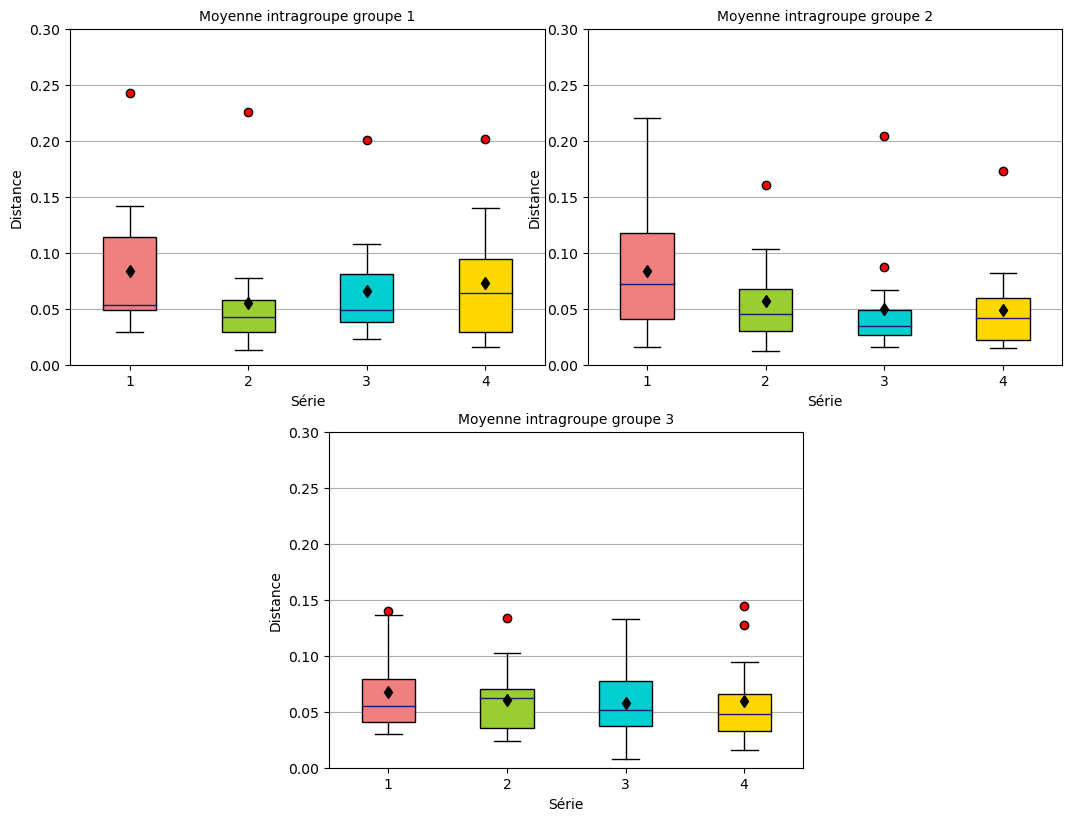
\includegraphics[width=15cm]{expe_results/Align_arm_All_data_intragroupe.png}}
    \caption[Moyenne des distances du défaut \textit{align arm} en intra-groupe]{Moyenne des distances du défaut align arm par rapport au centroïde du cluster des bons mouvements de l'expert en intra-groupe.}
    \label{fig:Align_arm_All_data_intragroupe}

	\centering
	\makebox[\textwidth][c]{
    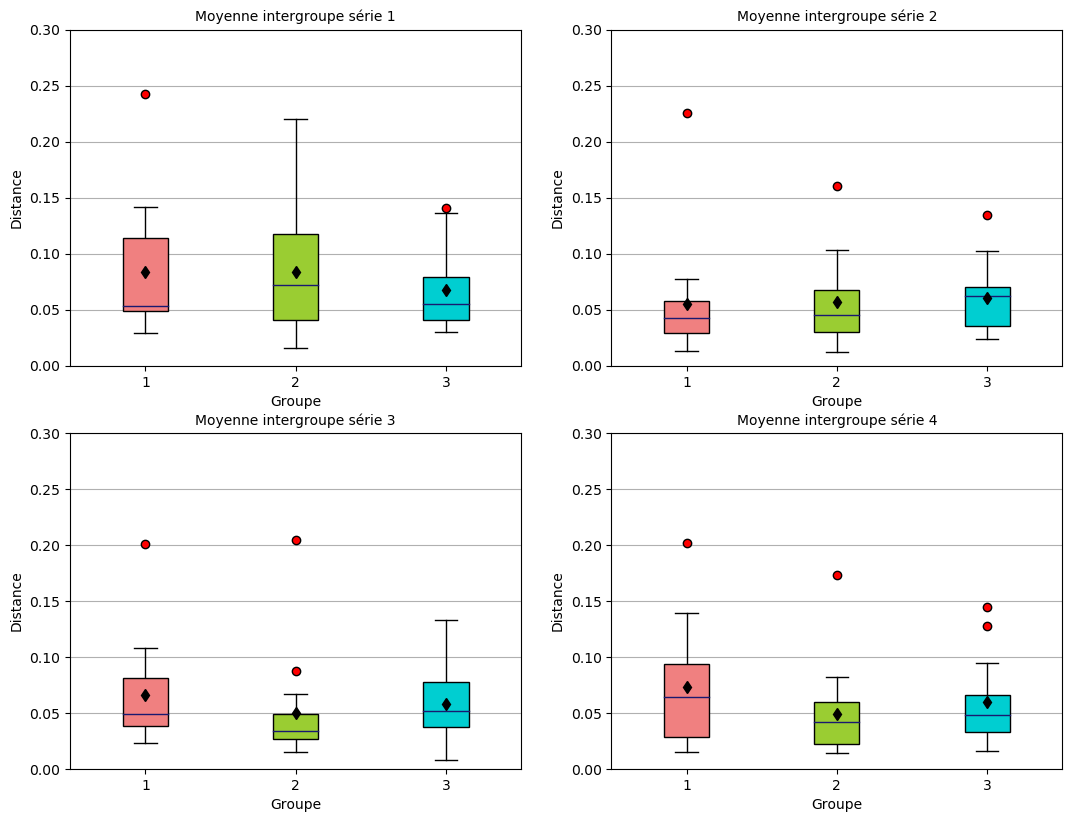
\includegraphics[width=15cm]{expe_results/Align_arm_All_data_intergroupe.png}}
    \caption[Distance du défaut \textit{align arm} en inter-groupe]{Moyenne des distances du défaut align arm par rapport au centroïde du cluster des bons mouvements de l'expert en inter-groupe.}
    \label{fig:Align_arm_All_data_intergroupe}
\end{figure}


\paragraph{Elbow move}

Le tableau \ref{tab:moy_std_elbow_move} présente les moyennes et les écarts-types de la distance des données des participants par rapport au centroïde du cluster des bons gestes de l'expert, pour le défaut du mouvement du coude. Il y a une amélioration systématique de ces valeurs entre le jeu 1 et le jeu 2, puis une stabilisation, sauf pour le groupe 3, où l'écart-type diminue encore entre le jeu 2 et le jeu 3. Cela indique une bonne prise en compte de ce conseil lorsqu'il est donné, ou qu'un conseil sur un autre défaut permet également de corriger le mouvement du coude.

\begin{table}[H]
\small
\makebox[\textwidth][c]{
\begin{tabular}{l|llllllll}
 & \multicolumn{2}{c}{Jeu 1} & \multicolumn{2}{c}{Jeu 2} & \multicolumn{2}{c}{Jeu 3} & \multicolumn{2}{c}{Jeu 4} \\\hline
 & Moyenne & Écart-Type & Moyenne & Écart-Type & Moyenne & Écart-Type & Moyenne & Écart-Type \\
Groupe 1 & 0.1174 & 0.0653 & 0.0527 & 0.0275 & 0.0544 & 0.0247 & 0.0547 & 0.0266 \\
Groupe 2 & 0.0932 & 0.0519 & 0.0566 & 0.0274 & 0.0453 & 0.0236 & 0.0453 & 0.0267 \\
Groupe 3 & 0.1092 & 0.0655 & 0.0575 & 0.0432 & 0.0492 & 0.0296 & 0.0552 & 0.0325
\end{tabular}}
\caption{Moyennes et écarts-types des données des apprenants (mouvement du coude).}
\label{tab:moy_std_elbow_move}
\end{table}

Les résultats intergroupes pour le défaut du mouvement du coude sont présentés dans la figure \ref{fig:Elbow_move_All_data_intergroupe}, et les résultats en intragroupe sont présentés dans la figure \ref{fig:Elbow_move_All_data_intragroupe}.


Lors de l'analyse intragroupe (figure \ref{fig:Elbow_move_All_data_intragroupe}), on peut constater une forte réduction de la valeur de la médiane, de l'écart interquartile et de la dispersion dès le jeu 2 pour tous les groupes. Les valeurs restent ensuite sensiblement les mêmes, autant pour la valeur de la médiane que de l'écart interquartile et la dispersion. Cette réduction peut être interprétée de deux manières : soit le défaut est systématiquement décelé par le système dès les premiers lancers, et sa correction est facilement effectuée par l'apprenant, soit un autre défaut souvent détecté par le système lors du premier jeu influence le défaut du mouvement du coude. Des valeurs significatives sont obtenues pour tous les groupes entre les jeux 1-2, 1-3 et 1-4 (table \ref{tab:elbow_move_intra}), confirmant ainsi l'amélioration nette du défaut entre le premier et le dernier jeu. Le groupe 2 obtient des résultats significatifs entre les jeux 2-3 et 2-4, suggérant ainsi que l'amélioration entre le jeu 3 et le jeu 4 est plus marginale. Enfin, le groupe 3 obtient des résultats significatifs entre le jeu 3 et le jeu 4, montrant une amélioration jusqu'au dernier jeu. Le groupe 1 présente trois données aberrantes pour le premier jeu, qui disparaissent ensuite pour les jeux suivants. Le groupe 3 semble contenir quelques apprenants ayant des difficultés avec le mouvement du coude (présence d'une ou deux données aberrantes sur chaque jeu).

L'analyse intergroupe (figure \ref{fig:Elbow_move_All_data_intergroupe}) permet d'observer que la valeur de la médiane et l'écart interquartile sont les plus faibles pour les groupes faisant intervenir le système (groupes 2 et 3). La dispersion reste sensiblement la même pour tous les groupes pour les jeux 2 et 3. L'observation effectuée sur l'analyse intragroupe se confirme ici, montrant que les différences intergroupes sont faibles dès le jeu 2. Les données intergroupes ne présentent pas de différences significatives (table \ref{tab:elbow_move_inter}).

\afterpage{
\begin{landscape}
\begin{table}[]
\centering
\begin{tabular}{ll|ccccc|cccc}
    &  & \multicolumn{5}{c|}{Wilcoxon Signed-Rank ($p < 0.05$)} & \multicolumn{4}{c}{T Test ($p < 0.05$)} \\ \cline{3-11}
    &  & \multicolumn{2}{c|}{One tail} & \multicolumn{2}{c}{Two tails} &  & \multirow{2}{*}{One tail} & \multirow{2}{*}{Two tails} & \multirow{2}{*}{t} & \multirow{2}{*}{df} \\ \cline{3-7}
    &  & p-norm & p-exact & p-norm & p-exact & T &  &  &  &  \\ \hline
   \multirow{3}{*}{Jeu 1-2} & G1 & \cellcolor{green!25} $6.6602e^{-4}$ & \cellcolor{green!25} $1.5259e^{-4}$ & \cellcolor{green!25} 0.0013 & \cellcolor{green!25} $3.0518e^{-4}$ & 3 &  &  &  &  \\
    & G2 & \cellcolor{green!25} $9.8276e^{-4}$ & \cellcolor{green!25} $3.0518e^{-4}$ & \cellcolor{green!25} 0.0020 & \cellcolor{green!25} $6.1035e^{-4}$ & 5 & \cellcolor{green!25} 0.0026 & \cellcolor{green!25} 0.0052 & 3.3014 & 14 \\
    & G3 & \cellcolor{green!25} $4.4595e^{-4}$ & \cellcolor{green!25} $6.1035e^{-5}$ & \cellcolor{green!25} $8.9190e^{-4}$ & \cellcolor{green!25} $1.2207e^{-4}$ & 1 &  &  &  &  \\ \hline
   \multirow{3}{*}{Jeu 2-3} & G1 &  &  &  &  &  & 0.3617 & 0.7235 & -0.3910 & 14 \\
    & G2 & 0.0738 & 0.0757 & 0.1475 & 0.1514 & 34 & \cellcolor{green!25} 0.0482 & 0.0964 & 1.7820 & 14 \\
    & G3 & 0.0661 & 0.0677 & 0.1323 & 0.1354 & 33 &  &  &  &  \\ \hline
   \multirow{3}{*}{Jeu 3-4} & G1 &  &  &  &  &  & 0.4712 & 0.9425 & -0.0735 & 14 \\
    & G2 & 0.3991 & 0.4020 & 0.7983 & 0.8039 & 55 &  &  &  &  \\
    & G3 & \cellcolor{green!25} 0.0416 & \cellcolor{green!25} 0.0416 & 0.0832 & 0.0832 & 29 &  &  &  &  \\ \hline
   \multirow{3}{*}{Jeu 1-3} & G1 & \cellcolor{green!25}$3.6326e^{-4}$ & \cellcolor{green!25}$3.0518e^{-5}$ & \cellcolor{green!25}$7.2651e^{-4}$ & \cellcolor{green!25}$6.1035e^{-5}$ & 0 &  &  &  &  \\
    & G2 & \cellcolor{green!25}0.0038 & \cellcolor{green!25}0.0021 & \cellcolor{green!25}0.0076 & \cellcolor{green!25}0.0043 & 12.5 & \cellcolor{green!25}0.0018 & \cellcolor{green!25}0.0036 & 3.4882 & 14 \\
    & G3 & \cellcolor{green!25}0.0014 & \cellcolor{green!25}$5.7983e^{-4}$ & \cellcolor{green!25}0.0029 & \cellcolor{green!25}0.0012 & 7 &  &  &  &  \\ \hline
   \multirow{3}{*}{Jeu 2-4} & G1 &  &  &  &  &  & 0.3837 & 0.7675 & -0.3015 & 14 \\
    & G2 &  &  &  &  &  & \cellcolor{green!25} 0.0263 & 0.0525 & 2.1182 & 14 \\
    & G3 & 0.4435 & 0.4452 & 0.8871 & 0.8904 & 57 & 0.3351 & 0.6702 & 0.4350 & 14 \\ \hline
   \multirow{3}{*}{Jeu 1-4} & G1 & \cellcolor{green!25} $6.6602e^{-4}$ & \cellcolor{green!25} $1.5259e^{-4}$ & \cellcolor{green!25} 0.0013 & \cellcolor{green!25} $3.0518e^{-4}$ & 3 &  &  &  &  \\
    & G2 & \cellcolor{green!25} $6.6602e^{-4}$ & \cellcolor{green!25} $1.5259e^{-4}$ & \cellcolor{green!25} 0.0013 & \cellcolor{green!25} $3.0518e^{-4}$ & 3 & \cellcolor{green!25} 0.0015 & \cellcolor{green!25} 0.0030 & 3.5854 & 14 \\
    & G3 & \cellcolor{green!25} $5.4581e^{-4}$ & \cellcolor{green!25} $9.1553e^{-5}$ & \cellcolor{green!25} 0.0011 & \cellcolor{green!25} $1.8311e^{-4}$ & 2 &  &  &  &
   \end{tabular}
\caption{Résultats des tests statistique en intragroupe (mouvement du coude).}
\label{tab:elbow_move_intra}
\end{table}
\end{landscape}}

\begin{table}[]
\begin{tabular}{lr|cccc}
    &  & Jeu 1 & Jeu 2 & Jeu 3 & Jeu 4 \\\hline
    \multirow{2}{*}{ANOVA} &  &  &  &  &  \\
     &  &  &  &  &  \\\hline
    \multirow{3}{*}{Pairwise T-test} & & & & & \\
     & & & & &  \\
     & & & & &  \\\hline
\multirow{3}{*}{Kruskal-Wallis ($p < 0.05$)} & Chi-square & 0.9793 & 0.2319 & 1.0321 & 0.5969 \\
 & p & 0.6128 & 0.8905 & 0.5969 & 0.4460 \\
 & df & 2 & 2 & 2 & 2 \\\hline
 \multirow{3}{*}{Pairwise Mann-Whitney} & & & & & \\
 & & & & & \\
 & & & & &
\end{tabular}
\caption{Résultats des tests statistiques en intergroupe (mouvement du coude).}
\label{tab:elbow_move_inter}
\end{table}

\begin{figure}%[H]
    \centering
    \makebox[\textwidth][c]{
    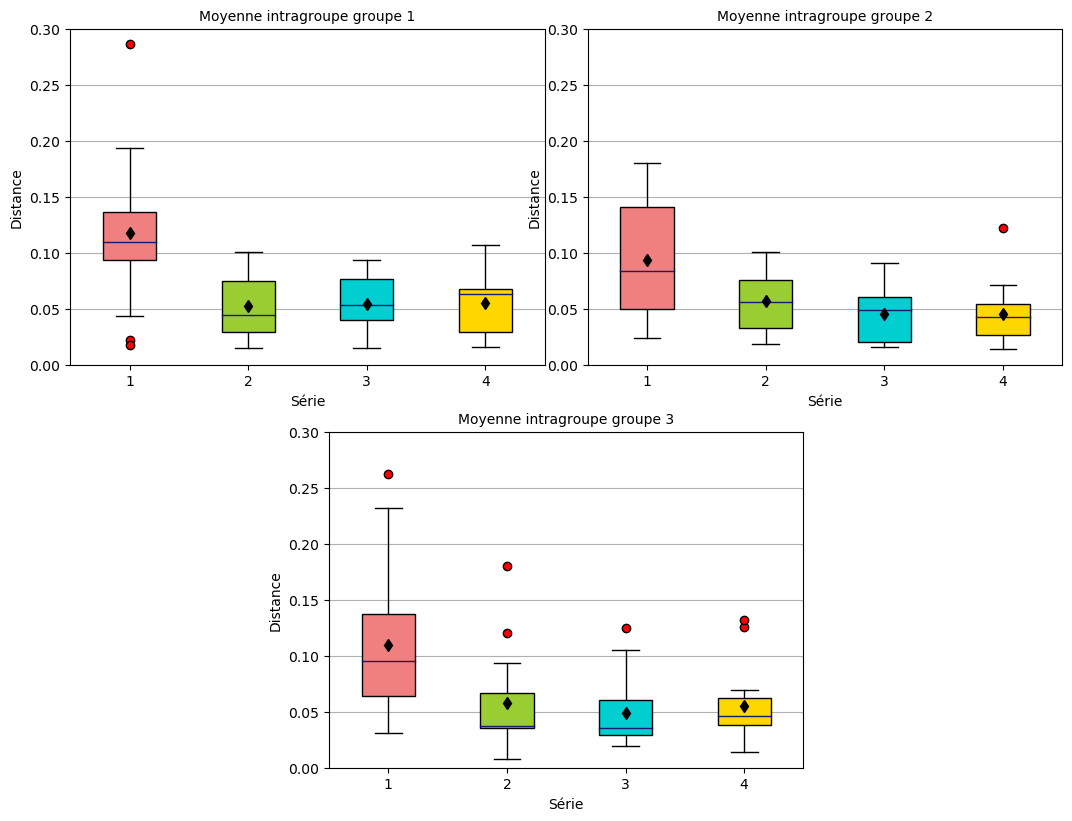
\includegraphics[width=15cm]{expe_results/Elbow_move_All_data_intragroupe.png}}
    \caption[Moyenne des distances du défaut \textit{elbow move} en intra-groupe]{Moyenne des distances du défaut \textit{elbow move} par rapport au centroïde du cluster des données de l'expert en intra-groupe}
    \label{fig:Elbow_move_All_data_intragroupe}

	\centering
	\makebox[\textwidth][c]{
    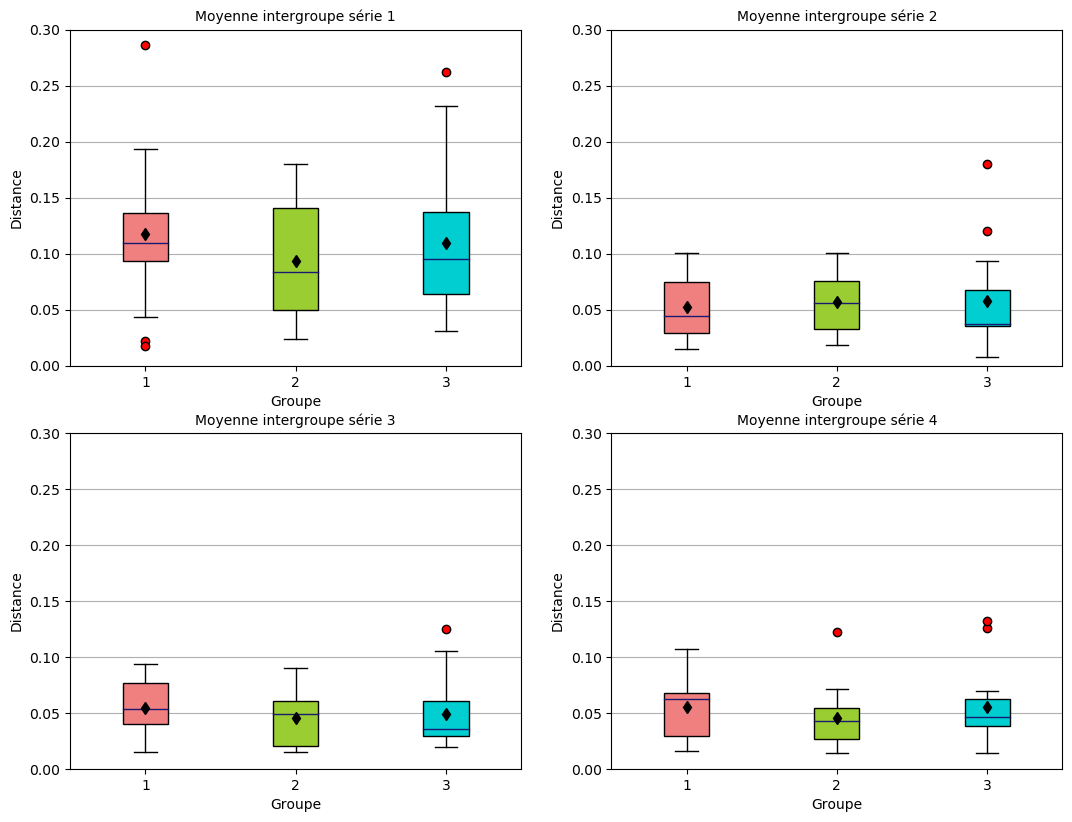
\includegraphics[width=15cm]{expe_results/Elbow_move_All_data_intergroupe.png}}
    \caption[Moyenne des distances du défaut \textit{elbow move} en inter-groupe]{Moyenne des distances du défaut \textit{elbow move} par rapport au centroïde du cluster des données de l'expert en inter-groupe.}
    \label{fig:Elbow_move_All_data_intergroupe}
\end{figure}


\paragraph{Javelin}

Le tableau \ref{tab:moy_std_javelin} présente les moyennes et les écarts-types de la distance des données des participants par rapport au centroïde des bons gestes de l'expert, pour le défaut du lancer type javelot. Il y a une amélioration de ces valeurs entre le jeu 1 et le jeu 2 pour tous les groupes, puis une stabilisation ensuite, sauf pour le groupe 2, où la moyenne diminue encore entre le jeu 3 et le jeu 4. Ces résultats suggèrent que la correction du défaut se fait dès le jeu 2, sans montrer d'amélioration par la suite, que le conseil soit donné ou non.

\begin{table}[H]
\small
\makebox[\textwidth][c]{
\begin{tabular}{l|llllllll}
 & \multicolumn{2}{c}{Jeu 1} & \multicolumn{2}{c}{Jeu 2} & \multicolumn{2}{c}{Jeu 3} & \multicolumn{2}{c}{Jeu 4} \\\hline
 & Moyenne & Écart-Type & Moyenne & Écart-Type & Moyenne & Écart-Type & Moyenne & Écart-Type \\
Groupe 1 & 0.1791 & 0.0720 & 0.1445 & 0.0798 & 0.1492 & 0.0658 & 0.1467 & 0.0689 \\
Groupe 2 & 0.1789 & 0.0594 & 0.1452 & 0.0718 & 0.1511 & 0.0888 & 0.1141 & 0.0513 \\
Groupe 3 & 0.1330 & 0.0513 & 0.1175 & 0.0321 & 0.1261 & 0.0314 & 0.1207 & 0.0375
\end{tabular}}
\caption{Moyennes et écarts-types des données des apprenants (mouvement du coude).}
\label{tab:moy_std_javelin}
\end{table}

Les résultats intergroupes pour le défaut du lancer type javelot sont présentés dans la figure \ref{fig:Javelin_All_data_intergroupe}, et les résultats en intragroupe sont présentés dans la figure \ref{fig:Javelin_All_data_intragroupe}.

Pour l'analyse intragroupe, la figure \ref{fig:Javelin_All_data_intragroupe} montre que la valeur de la médiane augmente sensiblement par au jeu 2 pour le groupe 1, suggérant une variabilité assez forte pour ce défaut. À l'inverse, pour le groupe 3, la valeur de la médiane, ainsi que l'écart interquartile, sont bas dès le jeu 1, et restent stables sur les autres. Pour le groupe 2, la valeur de la médiane baisse de manière continue, et l'écart interquartile, après une augmentation au jeu 2, diminue également au fur et à mesure des jeux. L'analyse statistique montre que les résultats sont significatifs pour le groupe 2 entre les jeux 1-3, 2-4, 1-4 et 3-4 (table \ref{tab:javelin_intra}) et pour le groupe 1 entre le jeu 1 et le jeu 2, confirmant ainsi le fait que le conseil est souvent donné par le système (voir tableau \ref{tab:advices_groupes_freq}) et que les apprenants réussissent à le corriger efficacement. Les données aberrantes présentes sur le jeu 1 du groupe 1 disparaissent dès le jeu 3. Le groupe 2 possède une donnée aberrante sur chaque jeu.

L'analyse intergroupe (figure \ref{fig:Javelin_All_data_intragroupe}) montre que le groupe 3 obtient systématiquement la meilleure dispersion pour l'ensemble des jeux, et les meilleures valeurs de médianes pour les deux premiers jeux. Le groupe 2 obtient les meilleures valeurs de médianes pour les deux derniers jeux. La stabilité de la valeur de la médiane, ainsi que l'écart interquartile bas dès le premier jeu suggère que le défaut n'était pas présent pour le groupe 3. La dispersion reste élevée pour le groupe 1 tout au long de l'expérimentation. Ces résultats ne présentent cependant pas de différences significatives (table \ref{tab:javelin_inter}).

\afterpage{
\begin{landscape}
\begin{table}[]
\centering
\begin{tabular}{ll|ccccc|cccc}
    &  & \multicolumn{5}{c|}{Wilcoxon Signed-Rank ($p < 0.05$)} & \multicolumn{4}{c}{T Test ($p < 0.05$)} \\ \cline{3-11}
    &  & \multicolumn{2}{c|}{One tail} & \multicolumn{2}{c}{Two tails} &  & \multirow{2}{*}{One tail} & \multirow{2}{*}{Two tails} & \multirow{2}{*}{t} & \multirow{2}{*}{df} \\ \cline{3-7}
    &  & p-norm & p-exact & p-norm & p-exact & T &  &  &  &  \\ \hline
   \multirow{3}{*}{Jeu 1-2} & G1 &  &  &  &  &  &\cellcolor{green!25}  0.0226 & \cellcolor{green!25} 0.0452 & 2.1984 & 14 \\
    & G2 &  &  &  &  &  & 0.0596 & 0.1192 & 1.6598 & 14 \\
    & G3 & 0.2755 & 0.2807 & 0.5509 & 0.5614 & 49 &  &  &  &  \\ \hline
   \multirow{3}{*}{Jeu 2-3} & G1 &  &  &  &  &  & 0.3370 & 0.6741 & -0.4295 & 14 \\
    & G2 & 0.2568 & 0.2622 & 0.5136 & 0.5245 & 48 &  &  &  &  \\
    & G3 &  &  &  &  &  & 0.1105 & 0.2209 & -1.2812 & 14 \\ \hline
   \multirow{3}{*}{Jeu 3-4} & G1 &  &  &  &  &  & 0.2455 & 0.4911 & 0.7071 & 14 \\
    & G2 & \cellcolor{green!25} 0.0029 & \cellcolor{green!25} 0.0017 & \cellcolor{green!25} 0.0059 & \cellcolor{green!25} 0.0034 & 11 &  &  &  &  \\
    & G3 &  &  &  &  &  & 0.2817 & 0.5635 & 0.5917 & 14 \\ \hline
   \multirow{3}{*}{Jeu 1-3} & G1 &  &  &  &  &  & 0.0739 & 0.1478 & 1.5322 & 14 \\
    & G2 & \cellcolor{green!25} 0.0191 & \cellcolor{green!25} 0.0177 & \cellcolor{green!25} 0.0381 & \cellcolor{green!25} 0.0353 & 23 &  &  &  &  \\
    & G3 & 0.4435 & 0.4452 & 0.8871 & 0.8904 & 57 &  &  &  &  \\ \hline
   \multirow{3}{*}{Jeu 2-4} & G1 &  &  &  &  &  & 0.4212 & 0.8424 & -0.2025 & 14 \\
    & G2 & \cellcolor{green!25} 0.0057 & \cellcolor{green!25} 0.0042 & \cellcolor{green!25} 0.0115 & \cellcolor{green!25} 0.0084 & 15 &  &  &  &  \\
    & G3 &  &  &  &  &  & 0.3671 & 0.7341 & -0.3465 & 14 \\ \hline
   \multirow{3}{*}{Jeu 1-4} & G1 &  &  &  &  &  & 0.0530 & 0.1061 & 1.7275 & 14 \\
    & G2 &  &  &  &  &  & \cellcolor{green!25} 0.0030 & \cellcolor{green!25} 0.0061 & 3.2280 & 14 \\
    & G3 & 0.2389 & 0.2443 & 0.4777 & 0.4887 & 47 &  &  &  &
   \end{tabular}
\caption{Résultats des tests statistiques en intragroupe (lancer de type javelot).}
\label{tab:javelin_intra}
\end{table}
\end{landscape}}

\begin{table}[]
    \begin{tabular}{lr|cccc}
        &  & Jeu 1 & Jeu 2 & Jeu 3 & Jeu 4 \\ \hline
       \multirow{2}{*}{ANOVA ($p < 0.05$)} & F (2, 42) & 2.6135 &  &  & 1.4252 \\
        & p & 0.0852 &  &  & 0.2518 \\ \hline
       \multirow{3}{*}{Pairwise T-test ($p < 0.05$)} &  &  &  &  &  \\
        &  &  &  &  &  \\
        &  &  &  &  &  \\ \hline
       \multirow{3}{*}{Kruskal-Wallis ($p < 0.05$)} & Chi-square &  & 0.8371 & 0.4924 &  \\
        & p &  & 0.6580 & 0.7818 &  \\
        & df &  & 2 & 2 &  \\ \hline
       \multirow{3}{*}{Pairwise Mann-Whitney ($p < 0.05$)} &  &  &  &  &  \\
        &  &  &  &  &  \\
        &  &  &  &  &
    \end{tabular}
\caption{Résultats des tests statistiques en intergroupe (lancer de type javelot).}
\label{tab:javelin_inter}
\end{table}

\begin{figure}%[H]
    \centering
    \makebox[\textwidth][c]{
    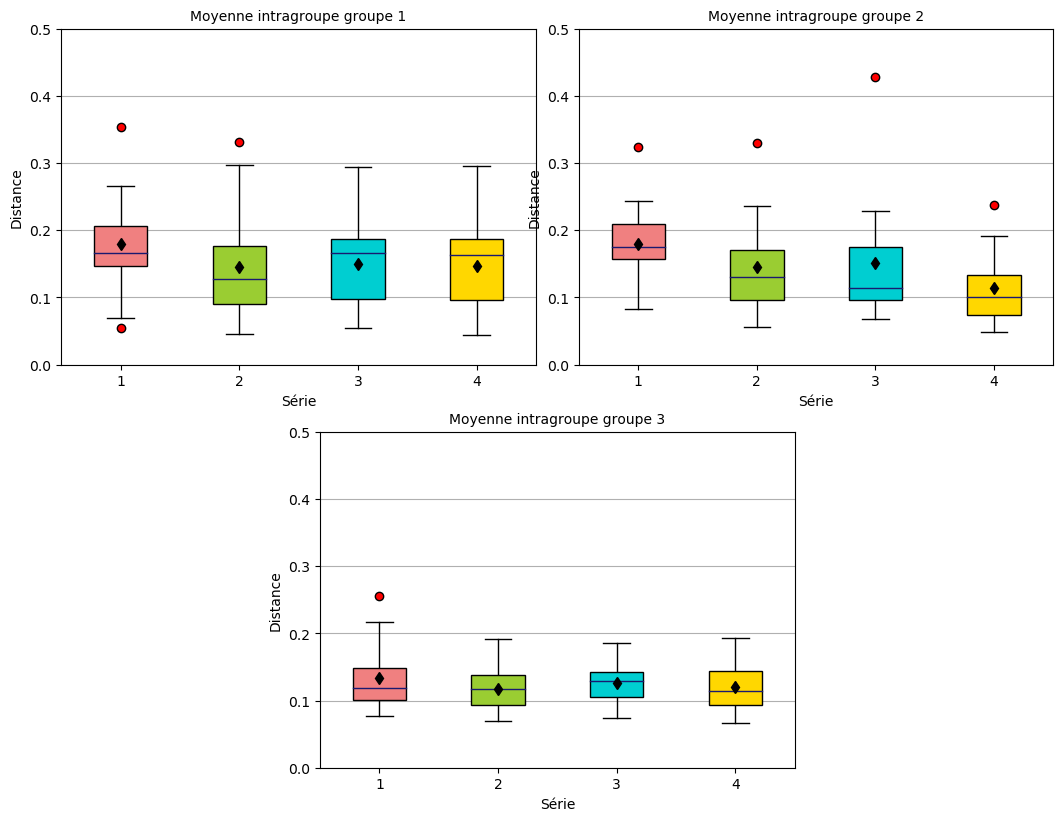
\includegraphics[width=15cm]{expe_results/Javelin_All_data_intragroupe.png}}
    \caption[Moyenne des distances du défaut \textit{javelin} en intra-groupe]{Moyenne des distances du défaut \textit{javelin} par rapport au centroïde du cluster des données de l'expert en intra-groupe}
    \label{fig:Javelin_All_data_intragroupe}

	\centering
	\makebox[\textwidth][c]{
    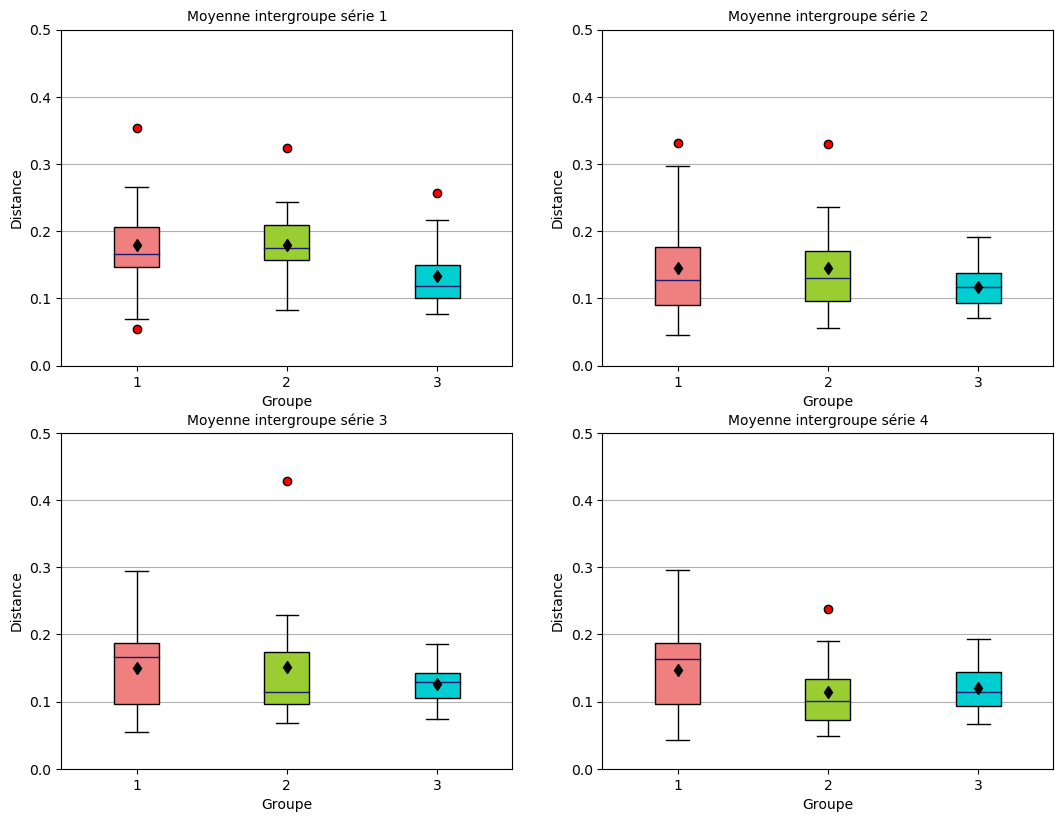
\includegraphics[width=15cm]{expe_results/Javelin_All_data_intergroupe.png}}
    \caption[Moyenne des distances du défaut \textit{javelin} en inter-groupe]{Moyenne des distances du défaut \textit{javelin} par rapport au centroïde du cluster des données de l'expert en inter-groupe.}
    \label{fig:Javelin_All_data_intergroupe}
\end{figure}

\paragraph{Leaning}

Le tableau \ref{tab:moy_std_leaning} présente les moyennes et les écarts-types de la distance des données des participants par rapport au centroïde des bons gestes de l'expert, pour le défaut du corps qui se penche. Il y a une forte amélioration de ces valeurs entre le jeu 1 et le jeu 2 pour tous les groupes, puis une stabilisation. Ces résultats suggèrent que la correction du défaut est effective dès le jeu 2.

\begin{table}[H]
\small
\makebox[\textwidth][c]{
\begin{tabular}{l|llllllll}
 & \multicolumn{2}{c}{Jeu 1} & \multicolumn{2}{c}{Jeu 2} & \multicolumn{2}{c}{Jeu 3} & \multicolumn{2}{c}{Jeu 4} \\\hline
 & Moyenne & Écart-Type & Moyenne & Écart-Type & Moyenne & Écart-Type & Moyenne & Écart-Type \\
Groupe 1 & 0.0813 & 0.0489 & 0.0359 & 0.0194 & 0.0359 & 0.0170 & 0.0354 & 0.0175 \\
Groupe 2 & 0.0557 & 0.0411 & 0.0351 & 0.0182 & 0.0265 & 0.0159 & 0.0270 & 0.0146 \\
Groupe 3 & 0.0725 & 0.0473 & 0.0370 & 0.0344 & 0.0322 & 0.0238 & 0.0369 & 0.0253
\end{tabular}}
\caption{Moyennes et écarts-types des données des apprenants (corps penché).}
\label{tab:moy_std_leaning}
\end{table}

Les résultats intergroupes pour le défaut du corps qui se penche lors du lancer sont présentés dans la figure \ref{fig:Leaning_All_data_intergroupe}, et les résultats en intragroupe sont présentés dans la figure \ref{fig:Leaning_All_data_intragroupe}.

Dans le cas de l'analyse intragroupe, la figure \ref{fig:Leaning_All_data_intragroupe} montre une forte baisse de l'écart interquartile, de la dispersion et de la valeur de la médiane pour les 3 groupes, et ce dès le jeu 2. Les valeurs restent ensuite stables, sauf pour le groupe 3, où l'écart interquartile se resserre progressivement jusqu'au jeu 3, à partir duquel il s'élargit de nouveau. Les résultats sont significatifs pour tous les groupes entre les jeux 1-3 et 1-4 (table \ref{tab:leaning_intra}), pour les groupes 1 et 3 entre le jeu 1 et le jeu 2, montrant une amélioration dès les premiers conseils donnés, et pour le groupe 2 entre les jeux 2-3 et 2-4, indiquant une progression plus étalée sur le temps. Ces résultats confirment ainsi la haute fréquence de ce conseil (tableau \ref{tab:advices_groupes_freq}) et l'amélioration systématique de ce défaut dans les mouvements des apprenants. Seule une donnée aberrante est présente (groupe 3), visible après le jeu 1.

Pour l'analyse intergroupe, la figure \ref{fig:Leaning_All_data_intergroupe} permet d'observer que l'écart interquartile est le meilleur pour le groupe 2 sur tous les jeux, ainsi que les valeurs des médianes sur les jeux 1 et 4 (très proches des valeurs des médianes du groupe 3). Le groupe 3 obtient une médiane sensiblement meilleure sur les jeux 2 et 4. La dispersion reste sensiblement la même quel que soit le groupe ou le jeu considéré. Aucun résultat ne présente une différence significative (tableau \ref{tab:leaning_inter}).

\afterpage{
\begin{landscape}
\begin{table}[]
\centering
\begin{tabular}{ll|ccccc|cccc}
    &  & \multicolumn{5}{c|}{Wilcoxon Signed-Rank ($p < 0.05$)} & \multicolumn{4}{c}{T Test ($p < 0.05$)} \\ \cline{3-11}
    &  & \multicolumn{2}{c|}{One tail} & \multicolumn{2}{c}{Two tails} &  & \multirow{2}{*}{One tail} & \multirow{2}{*}{Two tails} & \multirow{2}{*}{t} & \multirow{2}{*}{df} \\ \cline{3-7}
    &  & p-norm & p-exact & p-norm & p-exact & T &  &  &  &  \\ \hline
   \multirow{3}{*}{Jeu 1-2} & G1 & \cellcolor{green!25} $8.1026e^{-4}$ & \cellcolor{green!25} $2.1362e^{-4}$ & \cellcolor{green!25} 0.0016 & \cellcolor{green!25} $4.2725e^{-4}$ & 4 &  &  &  &  \\
    & G2 & 0.0592 & 0.0603 & 0.1183 & 0.1205 & 32 &  &  &  &  \\
    & G3 & \cellcolor{green!25} $9.8276e^{-4}$ & \cellcolor{green!25} $3.0518e^{-4}$ & \cellcolor{green!25} 0.0020 & \cellcolor{green!25} $6.1035e^{-4}$ & 5 &  &  &  &  \\ \hline
   \multirow{3}{*}{Jeu 2-3} & G1 &  &  &  &  &  & 0.4993 & 0.9986 & 0.0018 & 14 \\
    & G2 & \cellcolor{green!25} 0.0469 & \cellcolor{green!25} 0.047 & 0.0938 & 0.0946 & 30 & \cellcolor{green!25} 0.0336 & 0.0671 & 1.9845 & 14 \\
    & G3 & 0.2755 & 0.2807 & 0.5509 & 0.5614 & 49 &  &  &  &  \\ \hline
   \multirow{3}{*}{Jeu 3-4} & G1 &  &  &  &  &  & 0.4445 & 0.8891 & 0.1420 & 14 \\
    & G2 & 0.4435 & 0.4452 & 0.8871 & 0.8904 & 57 & 0.4438 & 0.8875 & -0.1440 & 14 \\
    & G3 & 0.0592 & 0.0603 & 0.1183 & 0.1205 & 32 &  &  &  &  \\ \hline
   \multirow{3}{*}{Jeu 1-3} & G1 & \cellcolor{green!25} $9.8276e^{-4}$ & \cellcolor{green!25} $3.0518e^{-4}$ & \cellcolor{green!25} 0.0020 & \cellcolor{green!25} $6.1035e^{-4}$ & 5 &  &  &  &  \\
    & G2 & \cellcolor{green!25} 0.0219 & \cellcolor{green!25} 0.0206 & \cellcolor{green!25} 0.0438 & \cellcolor{green!25} 0.0413 & 24 &  &  &  &  \\
    & G3 & \cellcolor{green!25} 0.0014 & \cellcolor{green!25} $5.7983e^{-4}$ & \cellcolor{green!25} 0.0029 & \cellcolor{green!25} 0.0012 & 7 &  &  &  &  \\ \hline
   \multirow{3}{*}{Jeu 2-4} & G1 & 0.4660 & 0.4670 & 0.9321 & 0.9341 & 58 & 0.4633 & 0.9266 & 0.0937 & 14 \\
    & G2 & \cellcolor{green!25} 0.0219 & \cellcolor{green!25} 0.0206 & \cellcolor{green!25} 0.0438 & \cellcolor{green!25} 0.0413 & 24 & \cellcolor{green!25} 0.0166 & \cellcolor{green!25} 0.0332 & 2.3622 & 14 \\
    & G3 & 0.4435 & 0.4452 & 0.8871 & 0.8904 & 57 &  &  &  &  \\ \hline
   \multirow{3}{*}{Jeu 1-4} & G1 & \cellcolor{green!25} 0.0014 & \cellcolor{green!25} $5.7983e^{-4}$ & \cellcolor{green!25} 0.0029 & \cellcolor{green!25} 0.0012 & 7 &  &  &  &  \\
    & G2 & \cellcolor{green!25} 0.0191 & \cellcolor{green!25} 0.0177 & \cellcolor{green!25} 0.0382 & \cellcolor{green!25} 0.0353 & 23 &  &  &  &  \\
    & G3 & \cellcolor{green!25} 0.0017 & \cellcolor{green!25} $7.6294e^{-4}$ & \cellcolor{green!25} 0.0034 & \cellcolor{green!25} 0.0015 & 8 &  &  &  &
\end{tabular}
\caption{Résultats des tests statistiques en intragroupe (corps penché).}
\label{tab:leaning_intra}
\end{table}
\end{landscape}}

\begin{table}[]
    \begin{tabular}{lr|cccc}
        &  & Jeu 1 & Jeu 2 & Jeu 3 & Jeu 4 \\ \hline
       \multirow{2}{*}{ANOVA ($p < 0.05$)} & F (2, 42) & 1.1188 &  &  &  \\
        & p & 0.3362 &  &  &  \\ \hline
       \multirow{3}{*}{Pairwise T-test ($p < 0.05$)} &  &  &  &  &  \\
        &  &  &  &  &  \\
        &  &  &  &  &  \\ \hline
       \multirow{3}{*}{Kruskal-Wallis ($p < 0.05$)} & Chi-square & 2.5484 & 0.7258 & 2.8197 & 1.3503 \\
        & p & 0.2796 & 0.6957 & 0.2442 & 0.5091 \\
        & df & 2 & 2 & 2 & 2 \\ \hline
       \multirow{3}{*}{Pairwise Mann-Whitney ($p < 0.05$)} &  &  &  &  &  \\
        &  &  &  &  &  \\
        &  &  &  &  &
    \end{tabular}
\caption{Résultats des tests statistiques en intergroupe (corps penché).}
\label{tab:leaning_inter}
\end{table}

\begin{figure}%[H]
    \centering
    \makebox[\textwidth][c]{
    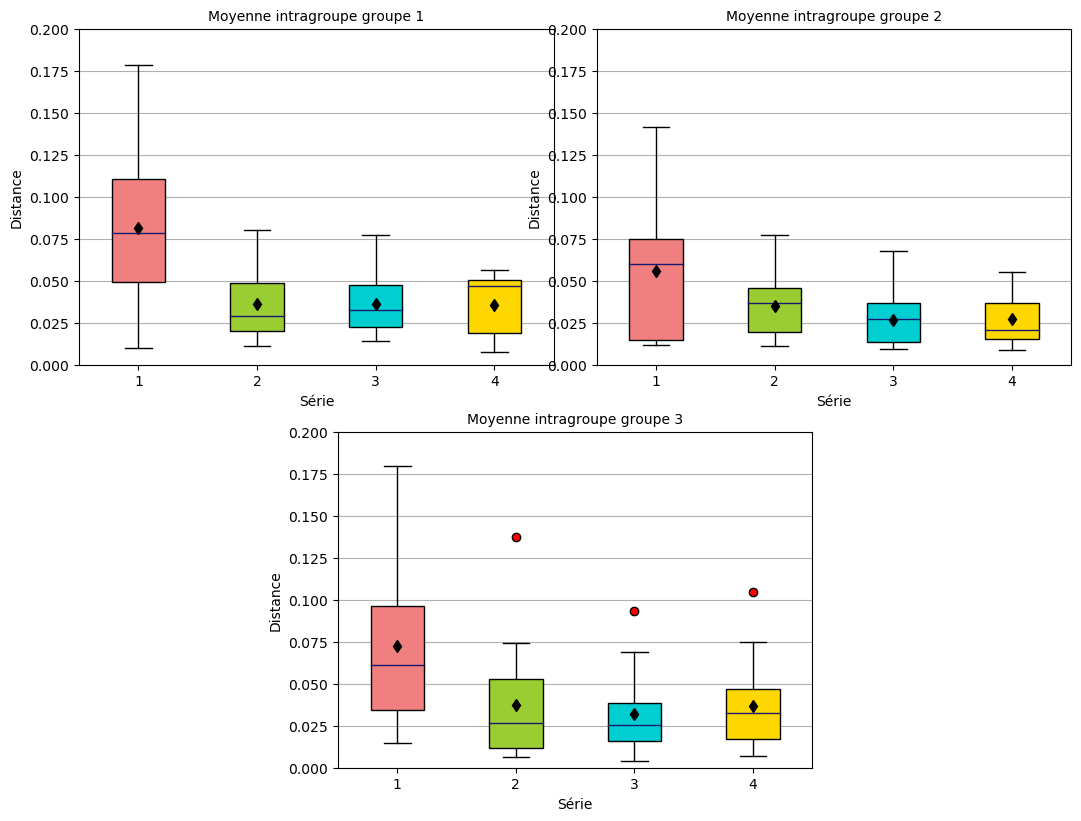
\includegraphics[width=15cm]{expe_results/Leaning_All_data_intragroupe.png}}
    \caption[Moyenne des distances du défaut \textit{leaning} en intra-groupe]{Moyenne des distances du défaut \textit{leaning} par rapport au centroïde du cluster des données de l'expert en intra-groupe}
    \label{fig:Leaning_All_data_intragroupe}

	\centering
	\makebox[\textwidth][c]{
    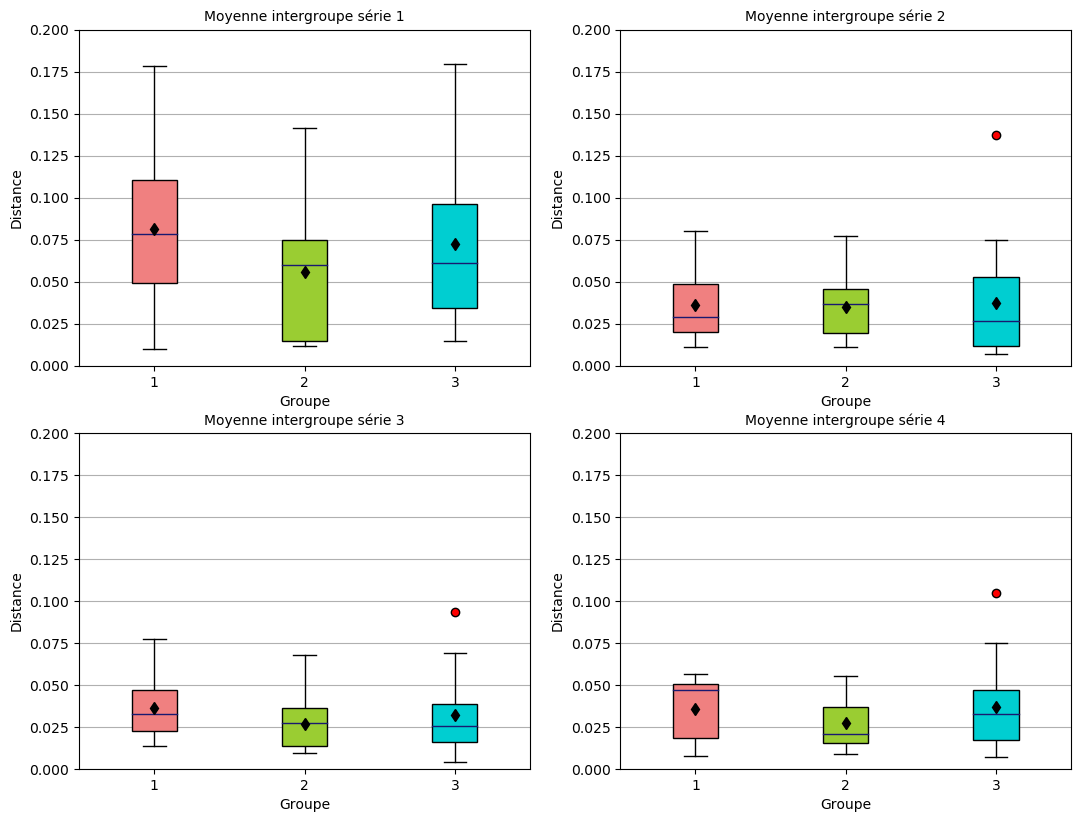
\includegraphics[width=15cm]{expe_results/Leaning_All_data_intergroupe.png}}
    \caption[Moyenne des distances du défaut \textit{leaning} en inter-groupe]{Moyenne des distances du défaut \textit{leaning} par rapport au centroïde du cluster des données de l'expert en inter-groupe.}
    \label{fig:Leaning_All_data_intergroupe}
\end{figure}

\paragraph{Tous les défauts pris ensemble}

Pour ce dernier cas, les gestes de l'apprenant sont comparés à ceux de l'expert dans leur entièreté (c'est-à-dire en utilisant tous les descripteurs calculés dans les autres cas). Les données sont concaténées, puis réduites à l'aide d'une analyse en composantes principales (avec $n = 2$), afin d'être cohérentes avec la visualisation en 2D proposée à l'expert.

Le tableau \ref{tab:moy_std_all} présente les moyennes et les écarts-types de la distance des données des participants par rapport au centroïde des bons gestes de l'expert, pour tous les défauts pris ensemble. Il y a une amélioration de ces valeurs entre le jeu 1 et le jeu 2 pour tous les groupes, puis une stabilisation ensuite, sauf pour le groupe 2, où la moyenne continue de baisser pour les jeux suivants. Ces résultats suggèrent que la correction des défauts est la plus grande dès les premiers conseils, puis que les ajustements sont discutables par la suite.

\begin{table}[H]
\small
\makebox[\textwidth][c]{
\begin{tabular}{l|llllllll}
 & \multicolumn{2}{c}{Jeu 1} & \multicolumn{2}{c}{Jeu 2} & \multicolumn{2}{c}{Jeu 3} & \multicolumn{2}{c}{Jeu 4} \\\hline
 & Moyenne & Écart-Type & Moyenne & Écart-Type & Moyenne & Écart-Type & Moyenne & Écart-Type \\
Groupe 1 & 2.0027 & 0.7263 & 1.1203 & 0.4826 & 1.1103 & 0.3991 & 1.1337 & 0.4221 \\
Groupe 2 & 1.6542 & 0.6728 & 1.0988 & 0.4676 & 0.9560 & 0.4468 & 0.8767 & 0.4177 \\
Groupe 3 & 1.7852 & 0.4966 & 1.0702 & 0.4587 & 1.0344 & 0.2784 & 1.1228 & 0.3482
\end{tabular}}
\caption{Moyennes et écarts-types des données des apprenants (tous les défauts).}
\label{tab:moy_std_all}
\end{table}

Les résultats intergroupes pour l'ensemble des défauts sont présentés dans la figure \ref{fig:distance_PCA_All_data_intergroupe}, et les résultats en intragroupe sont présentés dans la figure \ref{fig:distance_PCA_All_data_intragroupe}.

Dans le cas de l'analyse intragroupe, la figure \ref{fig:distance_PCA_All_data_intragroupe} montre une baisse de l'écart interquartile, de la dispersion et de la valeur de la médiane pour les 3 groupes, et ce dès le jeu 2. Les valeurs restent ensuite stables, sauf pour le groupe 3, où l'écart interquartile se resserre progressivement jusqu'au jeu 3, à partir duquel il s'élargit de nouveau, ainsi que pour les groupes 1 et 2 entre le jeu 3 et le jeu 4. Le groupe 2 montre une forte réduction de la dispersion au jeu 2, et varie peu par la suite. La réduction de la dispersion est plus lente pour les groupes 1 et 3, et se stabilise au niveau du jeu 3. Enfin, l'écart interquartile augmente entre le jeu 3 et le jeu 4, pour tous les groupes. Les résultats sont significatifs pour tous les groupes entre les jeux 1-2, 1-3 et 1-4, ainsi que pour le groupe 2 entre le jeu 2 et le jeu 4, et pour le groupe 3 entre le jeu 3 et le jeu 4, montrant une progression plus lente (table \ref{tab:distance_PCA_intra}).

Pour l'analyse intergroupe, la figure \ref{fig:distance_PCA_All_data_intergroupe} permet d'observer que bien que l'écart interquartile varie largement entre les différents groupes pour le jeu 1, les valeurs des médianes sont sensiblement les mêmes. Elles restent proches les unes des autres pour tous les jeux excepté le jeu 4, où la médiane du groupe 2 baisse alors que les deux autres augmentent. La médiane du groupe 2 est la meilleure dans tous les cas, sauf pour le jeu 2. Aucun résultat ne présente une différence significative (tableau \ref{tab:distance_PCA_inter}).

\afterpage{
\begin{landscape}
\begin{table}[]
\centering
\begin{tabular}{ll|ccccc|cccc}
    &  & \multicolumn{5}{c|}{Wilcoxon Signed-Rank ($p < 0.05$)} & \multicolumn{4}{c}{T Test ($p < 0.05$)} \\ \cline{3-11}
    &  & \multicolumn{2}{c|}{One tail} & \multicolumn{2}{c}{Two tails} &  & \multirow{2}{*}{One tail} & \multirow{2}{*}{Two tails} & \multirow{2}{*}{t} & \multirow{2}{*}{df} \\ \cline{3-7}
    &  & p-norm & p-exact & p-norm & p-exact & T &  &  &  &  \\ \hline
   \multirow{3}{*}{Jeu 1-2} & G1 &  &  &  &  &  & \cellcolor{green!25} $5.2824e^{-5}$ & \cellcolor{green!25} 0.0001 & 5.3330 & 14 \\
    & G2 & \cellcolor{green!25} 0.0067 & \cellcolor{green!25} 0.0051 & \cellcolor{green!25} 0.0135 & \cellcolor{green!25} 0.0102 & 16 & \cellcolor{green!25} 0.0031 & \cellcolor{green!25} 0.0064 & 3.2028 & 14 \\
    & G3 &  &  &  &  &  & \cellcolor{green!25} 0.0003 & \cellcolor{green!25} 0.0007 & 4.3281 & 14 \\ \hline
   \multirow{3}{*}{Jeu 2-3} & G1 & 0.3991 & 0.4020 & 0.7983 & 0.8039 & 55 & 0.4617 & 0.9234 & 0.0978 & 14 \\
    & G2 & 0.0528 & 0.0535 & 0.1055 & 0.1070 & 31 &  &  &  &  \\
    & G3 &  &  &  &  &  & 0.3554 & 0.7109 & 0.3783 & 14 \\ \hline
   \multirow{3}{*}{Jeu 3-4} & G1 &  &  &  &  &  & 0.3567 & 0.7135 & -0.3747 & 14 \\
    & G2 & 0.1221 & 0.1262 & 0.2443 & 0.2524 & 39 & 0.1262 & 0.2523 & 1.1940 & 14 \\
    & G3 &  &  &  &  &  & \cellcolor{green!25} 0.0435 & 0.0870 & -1.8404 & 14 \\ \hline
   \multirow{3}{*}{Jeu 1-3} & G1 &  &  &  &  &  & \cellcolor{green!25} $8.2423e^{-5}$ & \cellcolor{green!25} 0.0002 & 5.0895 & 14 \\
    & G2 & \cellcolor{green!25} 0.0092 & \cellcolor{green!25} 0.0075 & \cellcolor{green!25} 0.0184 & \cellcolor{green!25} 0.0151 & 18 & \cellcolor{green!25} 0.0037 & \cellcolor{green!25} 0.0073 & 3.1343 & 14 \\
    & G3 &  &  &  &  &  & \cellcolor{green!25} 0.0001 & \cellcolor{green!25} 0.0002 & 4.9613 & 14 \\ \hline
   \multirow{3}{*}{Jeu 2-4} & G1 & 0.3351 & 0.3394 & 0.6701 & 0.6788 & 52 & 0.4607 & 0.9214 & -0.1005 & 14 \\
    & G2 & \cellcolor{green!25} 0.0191 & \cellcolor{green!25} 0.0177 & \cellcolor{green!25} 0.0382 & \cellcolor{green!25} 0.0353 & 23 & \cellcolor{green!25} 0.0117 & \cellcolor{green!25} 0.0235 & 2.5419 & 14 \\
    & G3 &  &  &  &  &  & 0.2657 & 0.5314 & -0.6418 & 14 \\ \hline
   \multirow{3}{*}{Jeu 1-4} & G1 &  &  &  &  &  & \cellcolor{green!25} 0.0001 & \cellcolor{green!25} 0.0003 & 4.7662 & 14 \\
    & G2 & \cellcolor{green!25} 0.0029 & \cellcolor{green!25} 0.0017 & \cellcolor{green!25} 0.0059 & \cellcolor{green!25} 0.0034 & 11 & \cellcolor{green!25} 0.0012 & \cellcolor{green!25} 0.0023 & 3.7136 & 14 \\
    & G3 &  &  &  &  &  & \cellcolor{green!25} 0.0003 & \cellcolor{green!25} 0.0005 & 4.4723 & 14
\end{tabular}
\caption{Résultats des tests statistiques en intragroupe (tous les défauts).}
\label{tab:distance_PCA_intra}
\end{table}
\end{landscape}}



\begin{table}[]
    \begin{tabular}{lr|cccc}
        &  & Jeu 1 & Jeu 2 & Jeu 3 & Jeu 4 \\ \hline
       \multirow{2}{*}{ANOVA ($p < 0.05$)} & F (2, 42) & 1.0611 &  & 0.5728 & 1.8710 \\
        & p & 0.3551 &  & 0.5683 & 0.1666 \\ \hline
       \multirow{3}{*}{Pairwise T-test ($p < 0.05$)} &  &  &  &  &  \\
        &  &  &  &  &  \\
        &  &  &  &  &  \\ \hline
       \multirow{3}{*}{Kruskal-Wallis ($p < 0.05$)} & Chi-square &  & 0.0216 &  &  \\
        & p &  & 0.9892 &  &  \\
        & df &  & 2 &  &  \\ \hline
       \multirow{3}{*}{Pairwise Mann-Whitney ($p < 0.05$)} &  &  &  &  &  \\
        &  &  &  &  &  \\
        &  &  &  &  &
    \end{tabular}
\caption{Résultats des tests statistiques en intergroupe (tous les défauts).}
\label{tab:distance_PCA_inter}
\end{table}


\begin{figure}%[H]
    \centering
    \makebox[\textwidth][c]{
    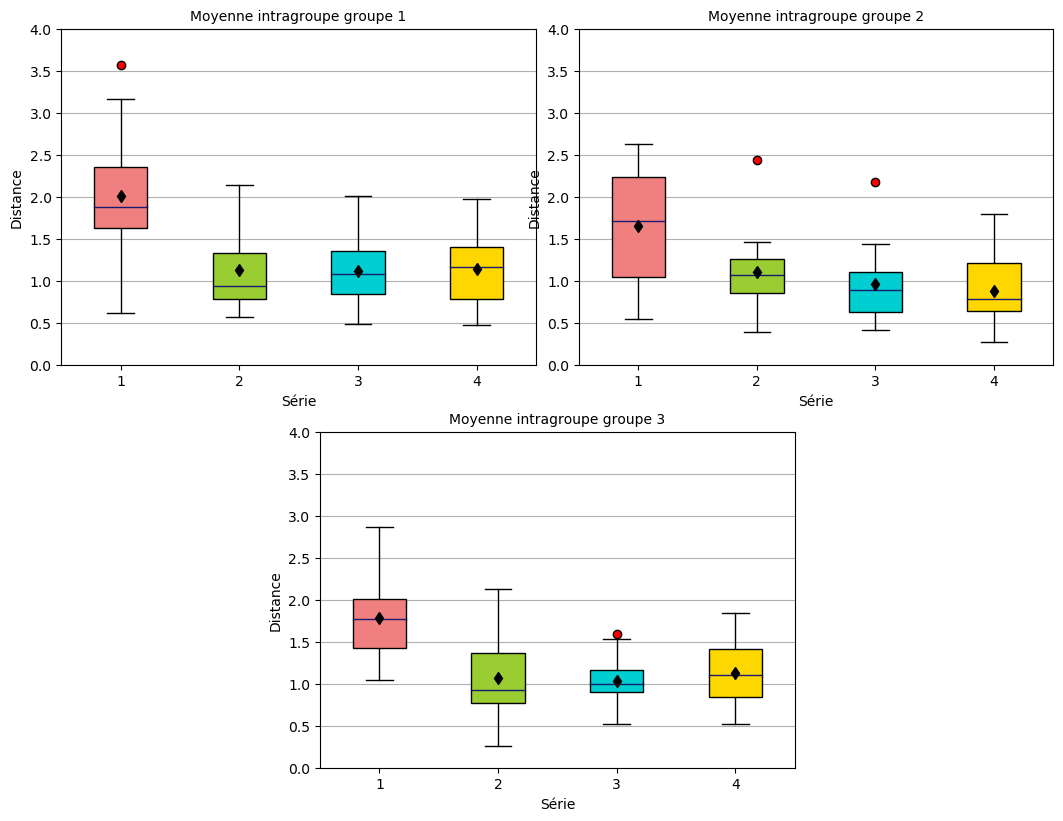
\includegraphics[width=15cm]{expe_results/Full_distance_PCA_All_data_intragroupe.png}}
    \caption[Moyenne des distances de tous les défauts en intra-groupe]{Moyenne des distances de tous les défauts par rapport au centroïde du cluster des données de l'expert en intra-groupe}
    \label{fig:distance_PCA_All_data_intragroupe}

	\centering
	\makebox[\textwidth][c]{
    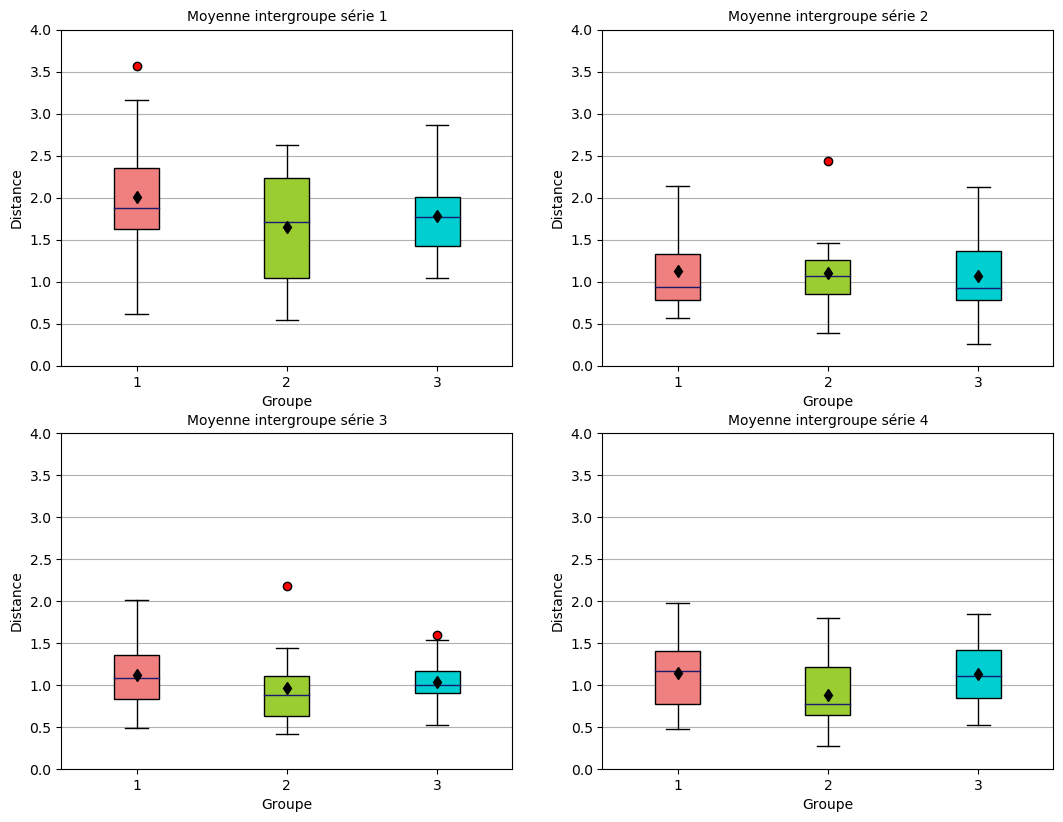
\includegraphics[width=15cm]{expe_results/Full_distance_PCA_All_data_intergroupe.png}}
    \caption[Moyenne des distances de tous les défauts en inter-groupe]{Moyenne des distances de tous les défauts par rapport au centroïde du cluster des données de l'expert en inter-groupe.}
    \label{fig:distance_PCA_All_data_intergroupe}
\end{figure}


\subsubsection{Corrélation entre les défauts et la précision}
Afin de vérifier s'il y a une corrélation entre la précision des lancers et l'amélioration des gestes, le $\tau$ de Kendall (tau de Kendall) a été calculé entre la précision et chaque défaut constaté du geste. Ce coefficient calcule la corrélation de rang entre deux variables $X$ et $Y$, et produit des valeurs pouvant varier de -1 à 1. Une valeur de 1 indique une corrélation positive totale, 0 indique qu'il n'y a aucune corrélation et -1 indique qu'il y a une corrélation négative totale. Les notations utilisées sont les suivantes :

\begin{itemize}[label=$-$]
	\item P : précision (distance par rapport au centre de la cible),
	\item A : alignement du bras,
	\item E : mouvement du coude,
	\item J : lancer type javelot,
	\item L : corps qui se penche,
	\item T : tous les descripteurs.
\end{itemize}

Les valeurs (ainsi que les p-values) des $\tau$ de Kendall sont données dans les tableaux \ref{tab:kendalltaup1}, \ref{tab:kendalltaup2} et \ref{tab:kendalltaup3}. L'hypothèse nulle ($p > 0.05$) indique que les variables sont indépendantes.

\begin{table}[H]
\centering
\resizebox{\linewidth}{!}{\begin{tabular}{l|cccccc}

& P & A & E & J & L & T\\ \hline
P & X & -0.1675 (0.0590) & \cellcolor{green!25} -0.2049 (0.0209) & -0.0175 (0.8432) & -0.1211 (0.1722) & \cellcolor{green!25} -0.1754 (0.0480)\\
A & -0.1675 (0.0590) & X & -0.0441 (0.6189) &  0.1079 (0.2231) & -0.0983 (0.2671) & -0.0407 (0.6461)\\
E & \cellcolor{green!25} -0.2049 (0.0209) & -0.0441 (0.6189) & X & \cellcolor{green!25} 0.3012 (0.0007) & \cellcolor{green!25} 0.7333 (0.0000) & \cellcolor{green!25} 0.6554 (0.0000)\\
J & -0.0175 (0.8432) &  0.1079 (0.2231) & \cellcolor{green!25} 0.3012 (0.0007) & X & \cellcolor{green!25} 0.2266 (0.0105) & \cellcolor{green!25} 0.4244 (0.0000)\\
L & -0.1211 (0.1722) & -0.0983 (0.2671) & \cellcolor{green!25} 0.7333 (0.0000) & \cellcolor{green!25} 0.2266 (0.0105) & X & \cellcolor{green!25} 0.6056 (0.0000)\\
T & \cellcolor{green!25} -0.1754 (0.0480) & -0.0407 (0.6461) & \cellcolor{green!25} 0.6554 (0.0000) & \cellcolor{green!25} 0.4244 (0.0000) & \cellcolor{green!25} 0.6056 (0.0000) & X\\

\end{tabular}}
\caption{Valeurs et p-values (entre parenthèses) des tau de Kendall entre les défauts du Groupe 1.}
\label{tab:kendalltaup1}
\end{table}

\begin{table}[H]
\centering
\resizebox{\linewidth}{!}{\begin{tabular}{l|cccccc}

& P & A & E & J & L & T\\ \hline
P & X &  0.0322 (0.7162) & -0.0639 (0.4711) &  0.0187 (0.8333) & -0.0718 (0.4179) & -0.1012 (0.2536)\\
A &  0.0322 (0.7162) & X &  0.1254 (0.1568) &  0.1345 (0.1290) &  0.0520 (0.5574) & \cellcolor{green!25} 0.2056 (0.0203)\\
E & -0.0639 (0.4711) &  0.1254 (0.1568) & X & \cellcolor{green!25} 0.3243 (0.0003) & \cellcolor{green!25} 0.7322 (0.0000) & \cellcolor{green!25} 0.6938 (0.0000)\\
J &  0.0187 (0.8333) &  0.1345 (0.1290) & \cellcolor{green!25} 0.3243 (0.0003) & X & \cellcolor{green!25} 0.2418 (0.0063) & \cellcolor{green!25} 0.4814 (0.0000)\\
L & -0.0718 (0.4179) &  0.0520 (0.5574) & \cellcolor{green!25} 0.7322 (0.0000) & \cellcolor{green!25} 0.2418 (0.0063) & X &  \cellcolor{green!25} 0.6565 (0.0000)\\
T & -0.1012 (0.2536) & \cellcolor{green!25} 0.2056 (0.0203) & \cellcolor{green!25} 0.6938 (0.0000) & \cellcolor{green!25} 0.4814 (0.0000) & \cellcolor{green!25} 0.6565 (0.0000) & X\\
\end{tabular}}
\caption{Valeurs et p-values (entre parenthèses) des tau de Kendall entre les défauts du Groupe 2.}
\label{tab:kendalltaup2}
\end{table}

\begin{table}[H]
\centering
\resizebox{\linewidth}{!}{\begin{tabular}{l|cccccc}

& P & A & E & J & L & T \\ \hline
P & X &  0.0368 (0.6784) & -0.0708 (0.4252) &  0.1274 (0.1512) & -0.0804 (0.3650) & -0.1240 (0.1624)\\
A &  0.0368 (0.6784) & X & \cellcolor{green!25} -0.1887 (0.0332)	&  0.0034 (0.9695) & -0.1057 (0.2330) & \cellcolor{green!25} 0.1751 (0.0480)\\
E & -0.0708 (0.4252) & \cellcolor{green!25} -0.1887 (0.0332) & X & -0.0554 (0.5319) & \cellcolor{green!25} 0.6889 (0.0000) & \cellcolor{green!25} 0.4734 (0.0000)\\
J &  0.1274 (0.1512) &  0.0034 (0.9695) & -0.0554 (0.5319) & X & -0.1532 (0.0839) & -0.1209 (0.1723)\\
L & -0.0804 (0.3650) & -0.1057 (0.2330)	& \cellcolor{green!25} 0.6889 (0.0000) & -0.1532 (0.0839) & X & \cellcolor{green!25} 0.5883 (0.0000)\\
T & -0.1240 (0.1624) & \cellcolor{green!25} 0.1751 (0.0480) & \cellcolor{green!25} 0.4734 (0.0000) & -0.1209 (0.1723) &  \cellcolor{green!25} 0.5883 (0.0000) & X\\

\end{tabular}}
\caption{Valeurs et p-values (entre parenthèses) des tau de Kendall entre les défauts du Groupe 3.}
\label{tab:kendalltaup3}
\end{table}

On remarque qu'aucune corrélation positive ou négative significative n'a été détectée entre la variation d'un défaut et la distance des fléchettes par rapport au centre de la cible, sauf pour le groupe 1 pour le mouvement du coude ($\tau = -0.2049$ et $p = 0.0209$) et la totalité des descripteurs ($\tau = -0.1754$ et $p = 0.0480$). Les valeurs des tau sont cependant faibles dans les deux cas. Cela indique que, dans le cadre de cette expérimentation, l'amélioration ou la détérioration d'un aspect du geste de l'apprenant n'est pas corrélé à l'amélioration ou la détérioration des autres aspects. Il y a cependant une corrélation forte entre le défaut du mouvement du coude et du corps qui se penche en avant pour tous les groupes ($\tau \approx 0.7$ et $p = 0$). Cela peut s'expliquer par la présence d'un descripteur commun aux deux défauts : la vitesse moyenne de l'épaule (du côté de la main dominante de l'apprenant). Ainsi, la correction du défaut du corps qui se penche en avant implique la diminution de cette valeur pour les deux défauts. Il existe également une forte corrélation entre le défaut du lancer type javelot et du mouvement du coude en avant pour les groupes 1 et 2, ainsi qu'entre le corps qui se penche et le lancer type javelot pour ces deux groupes.

Concernant la corrélation de tous les descripteurs ramenés en dimension 2 grâce à l'analyse en composantes principales, on remarque pour le groupe 1 une corrélation ($p = 0$) avec le mouvement du coude ($\tau = 0.6554$), le lancer javelot ($\tau = 0.4244$) et le corps qui se penche ($\tau = 0.6056$). Pour le groupe 2, la corrélation ($p = 0$) est avec le mouvement du coude ($\tau = 0.6938$), le lancer type javelot ($\tau = 0.4814$) et le corps penché lors du lancer ($\tau = 0.6565$). Enfin, pour le groupe 3, la plus grande corrélation ($p = 0$) est avec le mouvement du coude ($\tau = 0.4734$) et le corps penché lors du lancer ($\tau = 0.5883$). Ces résultats suggèrent que les caractéristiques les plus significatives pour l'analyse en composantes principales des mouvements varient pour chaque groupe, avec cependant en commun le mouvement du coude, ainsi que le corps penché lors du lancer. %Ces résultats peuvent apporter un premier élément de réponse pour l'explication et la détermination des caractéristiques du geste les plus importantes à corriger en premier, afin de se rapprocher du geste de l'expert : d'après les résultats, le rapprochement du geste de l'apprenant à celui de l'expert est fortement corrélé à l'amélioration des défauts du mouvement du coude ainsi que du corps penché lors du lancer.

\subsubsection{Réponses aux questionnaires}
La figure \ref{fig:graph_questionnaires} montre la répartition des réponses des participants, classées par ordre de satisfaction de très satisfait (7) à pas du tout satisfait (1). Le tableau \ref{darts_tab_survey} montre la moyenne des réponses des apprenants au pré-questionnaire et au post-questionnaire, par groupe et de manière globale. Parmi les 45 participants, aucun n'était expert du lancer de fléchettes, et la majorité d'entre eux avaient déjà joué aux fléchettes en tant que loisir (niveau aux fléchettes : $2.33 \pm 0.85$, 41 personnes ayant donné une réponse de 3 ou moins). Le niveau de stress des apprenants était systématiquement bas ($6,111 \pm 1,335$), avec un écart-type élevé dû à quelques apprenants stressés par le contexte de l'expérimentation. Les instructions données étaient claires et compréhensibles (niveau de compréhension des instructions reçues : $6.467 \pm 0.815$). L'auto-évaluation de la progression de la performance, ainsi que de la progression de la qualité du geste, présentent un écart-type élevé, montrant ainsi une difficulté à quantifier la progression par l'apprenant ($4.11 \pm 1.45$ pour la progression de la performance et $4.378 \pm 1.27$ pour la progression de la qualité du geste). Il semble que cet écart corresponde à une sous-évaluation quasi-systématique des apprenants. La corrélation linéaire calculée entre les réponses des différents groupes (tableau \ref{darts_tab_survey_correlation}) montre que, quel que soit le groupe, les réponses suivent toutes la même tendance. Ainsi, le ressenti de la progression du geste et de la précision, ainsi que de l'intérêt des conseils reçus, était le même, quel que soit le groupe considéré.

\begin{figure}
    \centering
    \makebox[\textwidth][c]{
    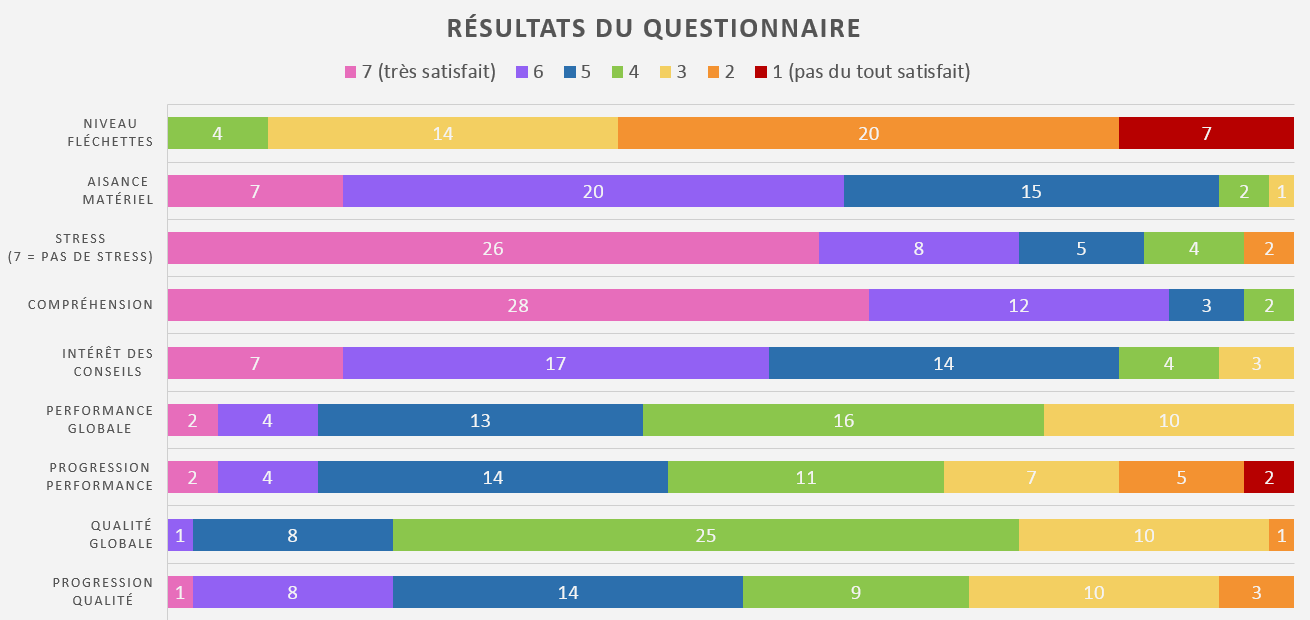
\includegraphics[width=15cm]{pictures/graph_questionnaires.png}}
    \caption[Résultats des questionnaires]{Le résultat des pré-/post-questionnaires par nombre de réponses pour chaque question, classées par ordre de satisfaction de très satisfait (7) à pas du tout satisfait (1).}
    \label{fig:graph_questionnaires}
\end{figure}


\begin{table}[h]
\centering
\begin{adjustbox}{max width=\textwidth}
\begin{tabular}{c|c|c|c|c|c|c|c|c|c|c}
 &  & \makecell[l]{Niveau\\Fléchettes} & \makecell[l]{Aisance\\Matériel} & \makecell[l]{Stress\\(7 = no stress)} & Compréhension & \makecell[l]{Intérêt\\des conseils} & \makecell[l]{Performance\\globale} & \makecell[l]{Progression\\Performance} & \makecell[l]{Qualité\\Globale} & \makecell[l]{Progression\\Qualité} \\ \hline
\multirow{2}{*}{G1} & Moyenne & 2,533 & 5,733 & 6,067 & 6,400 & 5,533 & 4,400 & 3,867 & 3,600 & 3,933 \\
 & Écart-type & 1,125 & 0,884 & 1,163 & 0,737 & 0,743 & 1,121 & 1,506 & 0,828 & 1,100 \\ \hline
\multirow{2}{*}{G2} & Moyenne & 2,200 & 5,400 & 6,133 & 6,600 & 5,200 & 4,600 & 4,133 & 3,933 & 4,533 \\
 & Écart-type & 0,775 & 1,056 & 1,457 & 0,828 & 1,014 & 1,242 & 1,727 & 0,799 & 1,506 \\ \hline
\multirow{2}{*}{G3} & Moyenne & 2,267 & 5,867 & 6,133 & 6,400 & 5,667 & 4,133 & 4,333 & 4,333 & 4,667 \\
 & Écart-type & 0,594 & 0,640 & 1,457 & 0,910 & 1,397 & 0,834 & 1,113 & 0,488 & 1,113 \\ \hline
\multirow{2}{*}{Tous} & Moyenne & 2,333 & 5,667 & 6,111 & 6,467 & 5,467 & 4,378 & 4,111 & 3,956 & 4,378 \\
 & Écart-type & 0,853 & 0,879 & 1,335 & 0,815 & 1,079 & 1,072 & 1,449 & 0,767 & 1,267
\end{tabular}
\end{adjustbox}
\caption{Moyenne et écart-type des réponses aux questions en fonction de chaque groupe.}
\label{darts_tab_survey}
\end{table}



\begin{table}[h]
\centering
\begin{tabular}{c|c|c|c}
Corrélations & G1 & G2 & G3 \\ \hline
G1 & 1 & 0,9668 & 0,9582 \\ \hline
G2 & 0,9668 & 1 & 0,9709 \\ \hline
G3 & 0,9582 & 0,9709 & 1
\end{tabular}
\caption{Indices de corrélations entre les moyennes des réponses aux questionnaires pour chaque groupe.}
\label{darts_tab_survey_correlation}
\end{table}

%\begin{table}[h]
%\centering
%\begin{adjustbox}{max width=\textwidth}
%\begin{tabular}{c|c|c|c|c|c|c|c|c|c}
% & \makecell[l]{Niveau\\Fléchettes} & \makecell[l]{Aisance\\Matériel} & \makecell[l]{Stress\\(7 = no stress)} & Compréhension & \makecell[l]{Intérêt\\des conseils} & \makecell[l]{Performance\\globale} & \makecell[l]{Progression\\Performance} & \makecell[l]{Qualité\\Globale} & \makecell[l]{Progression\\Qualité} \\ \hline
%G2 - G1 & -0,333 & -0,333 & 0,067 & 0,200 & -0,333 & 0,200 & 0,267 & 0,333 & 0,600 \\ \hline
%G3 - G1 & -0,267 & 0,133 & 0,067 & 0,000 & 0,133 & -0,267 & 0,467 & 0,733 & 0,733 \\ \hline
%G3 - G2 & 0,067 & 0,467 & 0,000 & -0,200 & 0,467 & -0,467 & 0,200 & 0,400 & 0,133
%\end{tabular}
%\end{adjustbox}
%\caption{Comparaison entre les groupes G2 et G1, G3 et G1 et G2 et G3 des moyennes des valeurs obtenues aux réponses du questionnaire.}
%\label{darts_tab_differnces_survey}
%\end{table}

\subsubsection{Discussion}
Des résultats significatifs ont été obtenus pour l'amélioration de certains défauts entre le jeu 1 et le jeu 4, à savoir les défauts \textit{leaning} et \textit{elbow move} pour tous les groupes, et \textit{javelin} et \textit{align arm} pour le groupe 2 seulement. Une explication possible est que ces deux derniers conseils n'ont pas été donnés par l'expert (c'est-à-dire la personne faisant passer les expérimentations), soit car d'autres défauts étaient plus proéminents, soit car ces défauts sont difficilement observables à l'œil nu. Ce dernier cas est plus susceptible d'arriver pour le groupe 1, où le système n'intervient pas. Il n'est pas possible d'utiliser une aide pour déterminer quels sont les défauts à corriger, lorsque l'observation à l'œil nu devient plus difficile. Ces résultats indiquent que les conseils donnés sont pertinents au regard des défauts considérés, et que les indicateurs calculés, ainsi que l'ensemble de règles choisies pour la sélection des conseils à donner, permettent de mettre en évidence les défauts du geste des apprenants, et ainsi les corriger. L'hypothèse \textbf{H4} est validée dans le contexte de cette expérimentation.

Les résultats de l'analyse de la corrélation des défauts entre eux, ainsi que de la distance par rapport au centre de la cible, montrent que l'amélioration de la distance des fléchettes par rapport au centre de la cible n'est pas corrélée avec l'amélioration du geste en lui-même. Cette observation est cohérente avec les résultats obtenus par d'autres études analysant le geste \parencite{LeNaour2019S3V, Ashford2006OME}. L'amélioration du geste se fait, dans un premier temps, au détriment de la précision du lancer. Cependant, il y a une dépendance, pour tous les groupes, entre le défaut du mouvement du coude et le défaut du corps qui se penche en avant, à cause de l'utilisation d'un descripteur commun. Ainsi, la correction d'un de ces deux défauts entraîne probablement une amélioration de l'autre.

La présence de données aberrantes persistantes sur l'ensemble des jeux pour certains défauts peut provenir d'un manque de conseil pour les défauts dans lesquels ils se trouvent. Ainsi, si d'autres défauts sont plus proéminents, l'expert ou le système ne donnera pas le conseil du défaut en question, et il n'y a pas d'amélioration du geste au regard de ce critère. Cela peut également indiquer que ce défaut n'est pas dépendant des autres, et que la correction d'autres défauts n'influence pas le défaut considéré.

Le défaut du lancer de type javelot présente une grande variabilité dans ses valeurs pour le groupe 1 (Fig. \ref{fig:Javelin_All_data_intragroupe} et \ref{fig:Javelin_All_data_intergroupe}). Cette variabilité pourrait s'expliquer par le fait que ce conseil n'est que très peu donné par l'expert, car plus difficilement visualisable que les autres.

Les analyses intergroupes ne permettent cependant pas de mettre en valeur une différence significative dans l'évolution du geste des apprenants au cours de l'expérimentation. Ainsi, l'expérimentation ne permet pas de conclure quant à l'amélioration de l'apprentissage du geste à l'aide du système développé en utilisation seule ou conjointement avec l'expert. Les hypothèses \textbf{H5} et \textbf{H6} n'ont pas été validées au cours de cette expérimentation.

\subsubsection{Limites de l'expérimentation}
Cette expérimentation, bien qu'ayant permis de montrer que le système permettait d'améliorer la correction des défauts des gestes des apprenants, présente plusieurs limites.

Tout d'abord, lors de la captation des gestes de l'expert, un phénomène d'auto-correction peut apparaître. Lorsque l'expert réalise des gestes présentant des défauts, l'enchaînement des captations peut mener à un certain manque d'attention et à un geste qui se rapproche du geste fait par l'expert en temps normal (c'est-à-dire le bon geste). Ainsi, la différence entre certains gestes bons et d'autres supposés mauvais peut apparaître comme étant très faible, voire invisible à l'œil nu. Ce problème est en partie pallié par l'utilisation du clustering, permettant de regrouper les gestes similaires ensemble.

Le nombre de lancers effectués (36) peut ne pas être suffisant pour pouvoir juger d'une évolution du mouvement sur la durée. Les processus d'apprentissage du geste nécessitent généralement plus de temps et de séances. Aussi, il peut être difficile d'obtenir des améliorations significatives lorsque l'on se base sur une seule séance de 36 lancers. De plus, entre chaque série de neuf lancers, il y avait une interruption afin que les données soient exportées puis traitées par le système. Cette limitation est propre au logiciel de traitement du mouvement Axis Neuron qui doit être utilisé lors de la captation avec la combinaison de capteurs, et non au système MLA. L'interruption des répétitions pendant quelques minutes peut mener à une « perte » de perception des caractéristiques du bon mouvement de l'apprenant, résultant ainsi en une perte de précision ou une dégradation de certains aspects du geste.

Une des limites du protocole expérimental exposé dans ce chapitre est qu'il en résulte systématiquement deux conseils à donner, même dans le cas où un seul (ou aucun) défaut est présent dans le geste. Ainsi, cela peut mener à une dégradation du geste sur la série suivante, car l'apprenant tente de corriger un défaut qui n'est pas ou plus présent. En pratique, ce cas ne s'est présenté que pour une seule série d'un apprenant.

Dans le cadre de l'expérimentation, l'analyse de l'expert est également plus difficile que dans un cadre d'apprentissage classique. En effet, le lancement et l'arrêt de la capture se font pour chaque lancer par l'expert, et cela implique une position proche du système informatique. Cette position ne permet pas de se déplacer autour de l'apprenant lors de la réalisation des gestes.

Dans un cadre d'apprentissage du lancer de fléchettes, l'expert analyse également des données extérieures au mouvement. Par exemple, le mauvais alignement du bras est détecté par l'expert en regardant la position des fléchettes sur la cible. L'expert donne comme tâche à l'apprenant de viser la partie « 20 » de la cible (localisé au milieu, allant du centre au bord supérieur de la cible) : si toutes les flèches tombent d'un côté, l'expert déduit que le bras penche vers ce côté lors du tir. Notre étude portant sur le geste en lui-même, nous avons dû définir des descripteurs provenant du geste de l'apprenant capable de mettre en relief ce défaut. D'autres analyses peuvent porter également sur le moment du lâcher de la fléchette, mais aussi sur la manière de la saisir avec les doigts.

Enfin, l'évaluation du système suppose que l'apprenant a systématiquement appliqué les conseils à la lettre ; en pratique, ce n'est pas toujours le cas. Les conseils peuvent soit être difficiles à comprendre pour l'apprenant, soit difficile à mettre en œuvre, et l'apprenant peut juger le conseil comme étant inutile pour l'amélioration de l'objectif du geste.


%Problèmes :
%\begin{itemize}
%\item Faible taille des échantillons pour les tests non-paramétriques
%	\item auto-correction de l'expert fait que les données sont parfois " bonnes " alors qu'elles devraient être " mauvaises " (corrigé en partie grâce au regroupement de ses données en clustering)
%	\item une seule séance avec peu de lancers (36 lancers), pas suffisant pour un réel apprentissage et potentiellement une réelle amélioration
%	\item Si tout est à peu près OK, sur-correction (car le système donne systématiquement 2 conseils quoiqu'il arrive), du coup dégradation du geste
%	\item interruption entre les neufs lancers (perte partielle du geste)
%	\item mouvements experts pas assez distincts pour certains défauts
%	\item expert analyse la cible en plus du geste (par exemple, alignement du bras)
%	\item Malgré le filtrage, les données sont parfois de mauvaise qualité (membre déplacés par exemple), non corrigeable (sauf à la main en modifiant le mouvement)
%	\item Données gaucher = très mauvaises
%	\item Conditions d'observations de l'expé difficiles (obligé d'être au pc pour l'enregistrement, du coup difficulté d'observer correctement le geste)
%	\item Le geste s'améliore parfois alors que la distance non
%	\item défauts leaning et align arm corrigent les autres défauts indirectement
%	\item Elbow move : le plus dur à corriger correctement (généralement, si le conseil est elbow move -> grosse dégradation des performances)
%	\item l'évaluation du système proposée suppose que l'apprenant a systématiquement appliqué les conseils à la lettre ; en pratique, ce n'est pas toujours le cas (si conseil appliqué -> amélioration, mais vu que les conseils ne sont pas tout le temps appliqués...)
%	\item Parfois l'apprenant a beaucoup de mal à prendre en compte un conseil, ce qui résulte soit en une perte de précision de ouf, soit en une non prise en compte du conseil
%\end{itemize}

\section{Synthèse des contributions}
Ce chapitre a présenté les trois expérimentations conduites dans le cadre de la validation du système MLA. Chaque expérimentation visait à vérifier une des facettes du système :
\begin{itemize}
	\item la capacité du système à séparer les gestes selon un étiquetage vérifiable par un humain à l'aide des descripteurs et des algorithmes choisis,
	\item la possibilité d'obtenir une séparation nette des données en deux clusters, correspondant au degré de réussite du geste,
	\item la capacité du système à assister l'enseignant dans sa tâche d'apprentissage d'un geste par l'analyse de ses besoins d'observation et démonstrations afin de déterminer et opérationnaliser les :
	\begin{itemize}
		\item descripteurs représentatifs du geste,
		\item propriétés de séparation des gestes acceptables de ceux qui ne le sont pas.
	\end{itemize}
\end{itemize}

Ces expérimentations ont ainsi permis de valider les hypothèses suivantes :
\begin{itemize}
    \item \textbf{H1} : Il est possible de regrouper les gestes selon leurs propriétés cinématiques communes.
	\item \textbf{H3} : Il est possible de séparer les gestes en fonction de propriétés attendues et identifiées au préalable par l'expert.
	\item \textbf{H4} : Il est possible de corriger chaque défaut du geste de l'apprenant, en lui indiquant les défauts majeurs à corriger en premier. Un défaut majeur est identifié par la plus grande distance séparant le mouvement courant de l'apprenant, du groupe de gestes acceptables ayant éliminé ce défaut.
\end{itemize}

Les hypothèses non-validées sont les suivantes :
\begin{itemize}
	\item \textbf{H2} : Il est possible de séparer les gestes des apprenants en deux groupes correspondant à une dichotomie geste réussi / geste raté afin de déterminer, pour une situation d'apprentissage donnée, les propriétés d'un ensemble fini de gestes réussis.
	\item \textbf{H5} : L'utilisation du système MLA basée sur l'hypothèse 4 permet d'améliorer l'apprentissage du geste par rapport à une situation sans le système MLA.
	\item \textbf{H6} : L'utilisation du système MLA en tant qu'assistant à l'enseignant permet d'améliorer l'apprentissage du geste par rapport à une situation sans MLA, et à une situation avec MLA et sans enseignant.
\end{itemize}

La première expérimentation a permis de montrer qu'il était possible d'obtenir une séparation acceptable (au sens des métriques calculées) des gestes de l'apprenant, en fonction des caractéristiques propres aux gestes observables par un humain. Bien qu'il ait été possible d'obtenir une séparation correcte dans la deuxième expérimentation, cette séparation ne correspondait pas à la dichotomie geste réussi / raté. Plusieurs pistes ont été évoquées pour expliquer ce résultat, par exemple l'absence d'une expertise du geste considéré, l'utilisation de descripteurs uniquement basés sur des propriétés cinématiques du geste. La troisième expérimentation a permis de vérifier si le système était capable d'assister un enseignant dans sa tâche d'enseignement d'un geste en intégrant ses besoins d'observation en tant que propriétés caractérisant les gestes d'une part, et permettant de regrouper les gestes acceptables et les gestes présentant les défauts préalablement identifiés d'autre part. Il y a eu une amélioration du geste dans tous les cas d'utilisation du système MLA (expert seul, système seul, expert assisté du système), avec une amélioration sur les quatre défauts considérés pour l'utilisation du système en autonomie. Cependant, il n'y a pas eu de différences significatives dans l'amélioration du geste entre les groupes.

L'amélioration de la distance par rapport au centre de la cible n'était cependant pas corrélée avec l'amélioration des défauts du geste. Ces résultats sont en accord avec ceux de la littérature \parencite{LeNaour2019S3V, Ashford2006OME}, qui montrent que l'amélioration du geste implique une perte de précision quant à l'objectif visé, dans le cadre du geste de lancers.

Les résultats obtenus au cours de la troisième expérimentation montrent que le système permet l'apprentissage du geste de manière autonome, ou d'assister l'expert dans sa tâche d'évaluation du geste. Cependant, dans le contexte de l'expérimentation, l'amélioration du geste n'était pas significativement meilleure (au sens des tests statistiques effectués) selon les différents groupes de participants. L'agrandissement de la population, afin d'obtenir des résultats plus fiables, ainsi que le test du système sur un autre geste, permettraient de confirmer ou d'infirmer ces tendances.


